\documentclass[german]{latex4ei_fs}
\usepackage[european]{circuitikz}
\author{Martin Zellner}
\myemail{zellnerm@ethz.ch}			% optional, delete if unchanged
	\fancyfoot[L]{ \EngGer{Please report mistakes \emph{immediately}}{Fehler bitte \emph{sofort} melden}.}

	\renewcommand{\fstitle}[1]{
		\vspace{-20mm}{
		
			\huge\textbf{#1}
		}
	}
\usepackage{pbox}
\begin{document}
\fstitle{Elektrische Antriebssysteme I} 

\section{Allgemeines}
\begin{sectionbox}
	\subsection{Einheiten}
	\begin{tablebox}{llll} 
		\textbf{Größe} & \textbf{Definition} & \textbf{Einheit} & \textbf{SI-Notation} \\ \cmrule
		%Geschwindigkeit & $\vec{v}=\frac{\mathrm d \vec{s}}{\mathrm dt}$ & $\frac{m}{s}$ & \\
		%Beschleunigung & $\vec{a}=\frac{\mathrm d \vec{v}}{\mathrm dt}$ & $\frac{m}{s^2}$ & \\
		Frequenz & $f = \frac{c}{\lambda}$ & Hertz & $\si{\hertz} = \si{ \per \second}$\\
		Kraft & $ \vec F := m \cdot \vec a $ & Newton & $\si{\newton} = \si{\kilogram \meter \per \second \squared}$\\
		Druck & $p := \frac{\vec F_\perp}{A}$ & Pascal & $\si{\pascal} = \si{\newton \per \meter \squared} = \si{\kilogram \per \meter \second \squared}$\\
		${}^{\textstyle \text{Arbeit,}}_{\textstyle \text{Energie}}$ & $W := \int \vec F \diff \vec s$ & Joule & $\si{\joule} = \si{\newton\meter} = \si{\kilogram\meter \squared \per \second \squared}$ \\
		Leistung & $P := \frac{\mathrm dW}{\mathrm dt}$ & Watt & $\si{\watt} = \si{\joule \per \second} = \si{\kilogram\meter \squared \per \second \cubed}$\\
		%Impuls & $\vec p := m \cdot \vec v$ & $\frac{kg\; m}{s}$ & \\
		Spannung & $U := \frac{W}{Q}$ & Volt & $\si{\volt} = \si{\watt \per \ampere} = \si{\kilogram\meter  \squared \per \ampere\second \cubed}$\\
		Ladung & $Q:= \int I \diff t$ & Coulomb & $\si{\coulomb} = \si{\ampere\second}$\\
		Resistivität & $R := \frac{\diff U}{\diff I}$ & Ohm & $\si{\ohm} = \si{\volt \per \ampere} = \si{\kilogram\meter  \squared \per \ampere  \squared\second \cubed}$\\
		Kapazität & $C:= \frac{\diff Q}{\diff U}$ & Farad & $\si{\farad} = \si{\coulomb \per \volt} = \si{\ampere  \squared  \second \tothe{4}\per \kilogram\meter \squared}$\\	
		Induktivität & $L := \frac{\diff \Phi}{\diff I}$ & Henry & $\si{\henry} = \si{\volt\second \per\ampere} = \si{\kilogram\meter  \squared \per \ampere  \squared \second  \squared}$\\
		${}^{\text{Magnetischer}}_{\textstyle \text{Fluss}}$ & $\Phi_{\ir M} := \int \vec B \diff \vec A$ & Weber & $\si{\weber} = \si{\volt\second} = \si{\kilogram\meter \squared \per \ampere\second \squared}$\\[0.2em]
		${}^{\text{Magnetische}}_{\textstyle \text{Flussdichte}}$ & $\vec B := \mu_0 \vec H$ & Tesla & $\si{\tesla} = \si{\weber \per \meter  \squared} = \si{\kilogram \per \ampere\second \squared}$\\
\end{tablebox}
\end{sectionbox}
\begin{sectionbox}
	\subsection{Newtonsche Mechanik $\vec F=m \vec a $}
	\begin{tablebox}{ccc} 
				& \large Translation & {\large Rotation} (Radius $r$) \\ \cmrule
		Strecke/Winkel & \large $\vec x$ & \large $\vec \varphi =  \frac{\vec x}{r}$\\[0.2em]
		Geschwindigkeit & \large $\vec v = \dot{\vec x}$ & \large $\vec \omega = \dot{\vec \varphi} = \frac{\vec v}{r}$ \\[0.2em]
		Beschleunigung & \large $\vec a = \dot{\vec v} = \ddot{\vec x}$ & \large $\vec \alpha = \dot{\vec \omega} = \ddot{\vec \varphi} = \frac{\vec a}{r}$ \\[0.2em]
		Masse/Trägh. & \large $m$ & \large $\Theta = \int_V \vec r^2_\perp \diff m$ \\[0.2em]
		Impuls/Drall & \large $\vec p =m \vec v$ & \large $\vec L = \ma \Theta \vec \omega = \vec r \times \vec p$ \\[0.2em]
		Kraft/Moment & \large $\vec F = \dot{\vec p} = m \vec a$ &  \large $\vec M = \dot{\vec L} = \ma \Theta \vec \alpha = \vec r \times \vec F$ \\[0.2em]
		Energie & \large $E_{\ir kin}=\frac12mv^2$ & \large $E_{\ir rot}=\frac12 \Theta \omega ^2$\\[0.2em]
		Leistung & \large $P = \vec F \bdot \vec v$ & \large $P = \vec M \bdot \vec \omega$\\ 
	\end{tablebox}
\end{sectionbox}
\begin{sectionbox}
	\subsection{Elektrische Felder}

	\subsubsection*{Maxwellsche Gleichungen (Naturgesetze)}
	\begin{tabular}{ll}
		Gaußsches Gesetz: & Faradaysches ind. Gesetz\\
		\large $\div \vec D = \varrho $ & \large $\rot \vec E + \frac{\partial \vec B}{\partial t} = 0$ \\[1em]
		Quellfreiheit des magn. Feldes & Ampèrsches Gesetz\\
		\large $\div \vec B = 0$ & \large $\rot \vec H = \vec j + \frac{\partial \vec D}{\partial t}$\\[0.3em]
	\end{tabular} 

	\begin{tabular}{lll} \ctrule
		\textbf{Resistiv} & \textbf{Kapazitiv} & \textbf{Induktiv}\\ \cmrule
		\large $\mathrm d I = G \diff U$ & \large $\mathrm d Q = C \diff U$ & \large $\mathrm d \Phi_M = L \diff I$\\[0.3em] 
		\large $\vec j = \sigma \vec E$ & \large $\vec D = \varepsilon \vec E$ & \large $\vec B = \mu \vec H$\\ [0.3em] 
		\large $\mathrm d I = \vec j \diff A$ & \large $\mathrm d U = \vec E \diff \vec r$ & \large $\mathrm d \Phi_M = \vec B \diff A$\\[0.3em]  
		\large $\vec j = q n \vec v$ & \large $Q(V) \equiv \oiint\limits_{\partial V}\! \vec D \diff \vec A\;$ & \large $I(A) \equiv \oint\limits_{\partial A}\! \vec H \diff\vec r$\\ \noalign{\vspace{2pt}}\cmrule
		Widerst. $R = \rho \frac{l}{A}$ & Kondensator $C=\varepsilon \frac{A}{d}$ & Spule $L=\mu A \frac{N^2}{l}$\\
		\cbrule
	\end{tabular}
\end{sectionbox}	
\begin{sectionbox}
\subsection{Komplexe Zahlen $\cx z \in \C = \R^2$}
\pbox{3cm}{ 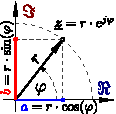
\includegraphics{./img/trigo.pdf} } \quad
\pbox{6cm}{ 
	$\cx z = \underset{\text{Karthesisch}}{a + b\i} = \underset{\text{Polarkoord.}}{r \cdot e^{\i \varphi}}$ \quad\ \boxed{ \underset{\text{Imaginäre Einheit}}{\i = \sqrt{-1}}}\\[0.4em] 
	$\i^{2n} = -1^n$ \quad\ $\i^{2n+1} = -\i^n$ \quad\ $\i^{-1} = -\i$ \\[0.2em] 
	$\ol{\cx z} = a - b\i$ \qquad $\cx z \ol{\cx z} = \abs{\cx z}^2 = a^2+b^2$\\[0.2em]
	$\cx z_1 \cdot \cx z_2 = r_1 \cdot r_2 \cdot e^{\i (\varphi_1 + \varphi_2)}$\\[0.2em]
	$z^{-1} = \frac{\ol{\cx z}}{\ol{\cx z} \cx z}=\frac{\ol{\cx z}}{a^2+b^2}$ }


\end{sectionbox}

\begin{sectionbox}
Leistungsfaktor: $\cos \varphi = \frac{P}{S}$
\end{sectionbox}
\section{Gleichstrommaschine}

\begin{sectionbox}

\subsection*{Elektrisch}

Ankerkreis: $U_a = U_i + R_a I_a + L_a \frac{\diff I_a}{ \diff t}$ \\
Erregerkreis: $U_e = R_e I_e + L_e \frac{\diff I_e}{\diff t}$

\subsection*{Mechanisch}
$M_{\ir el} = M_{\ir Welle} + M_R + J \frac{\diff \omega_m}{\diff t}$

\subsection*{Kopplung}
$U_i = c \Phi \omega_m$ \\
$M_{\ir el} = c \Phi I_a$ \quad mit $c$: Maschinenkonstante

Erregerfluss: $\Phi = \frac{L_e}{N_e} I_e$ \quad mit $N_e$: Windungszahl


\subsection*{Wirkungsgrad}
$\eta = \frac{P_m}{P_e} = \frac{M \omega_m}{U_a I_a + U_e I_e}$
\end{sectionbox}

\begin{sectionbox}
\subsection{Fremderregte Maschine}
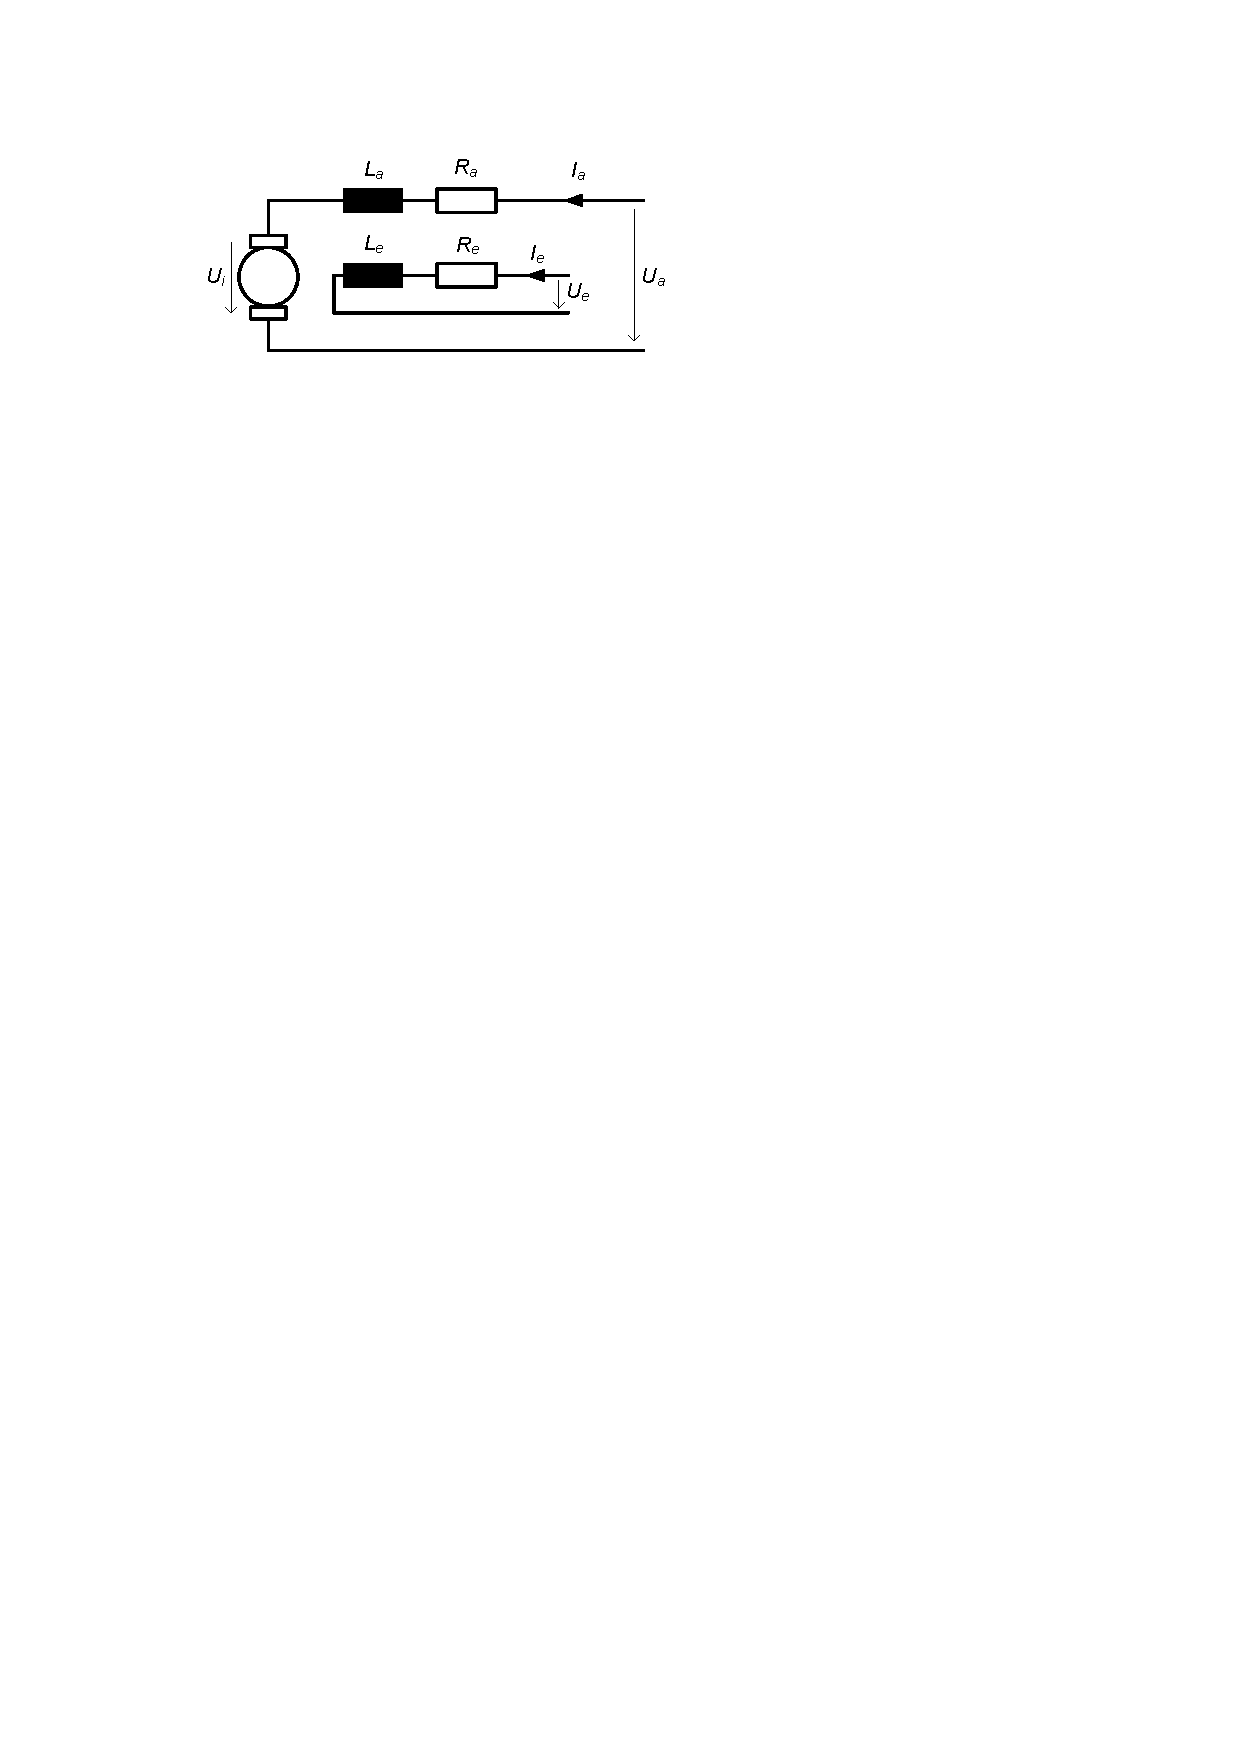
\includegraphics[width=0.6\columnwidth]{GM_F.pdf}

\subsubsection*{Stationärer Betrieb}
$\omega_m =  \frac{U_a - R_a I_a}{c \Phi} $ \\
$M_{\ir el} = c \cdot \Phi \cdot I_a$ \\

$\omega_m = \frac{U_a}{c \Phi} - \frac{R_a}{(c \Phi)^2} M_{\ir el}  $
\subsubsection*{Leerlauf}
 $M = 0 \Ra I_a = 0 \Ra U_a = U_i$ \\
 mechanische Kreisfrequenz: $\omega_{m0} = \frac{U_a}{c \Phi}$

 Leerlaufdrehzahl: $n_0 = \omega_{m0} \cdot \frac{60}{2 \pi}$ (U/min)
\end{sectionbox}
\begin{sectionbox}
\subsection{Nebenschlussmaschine}
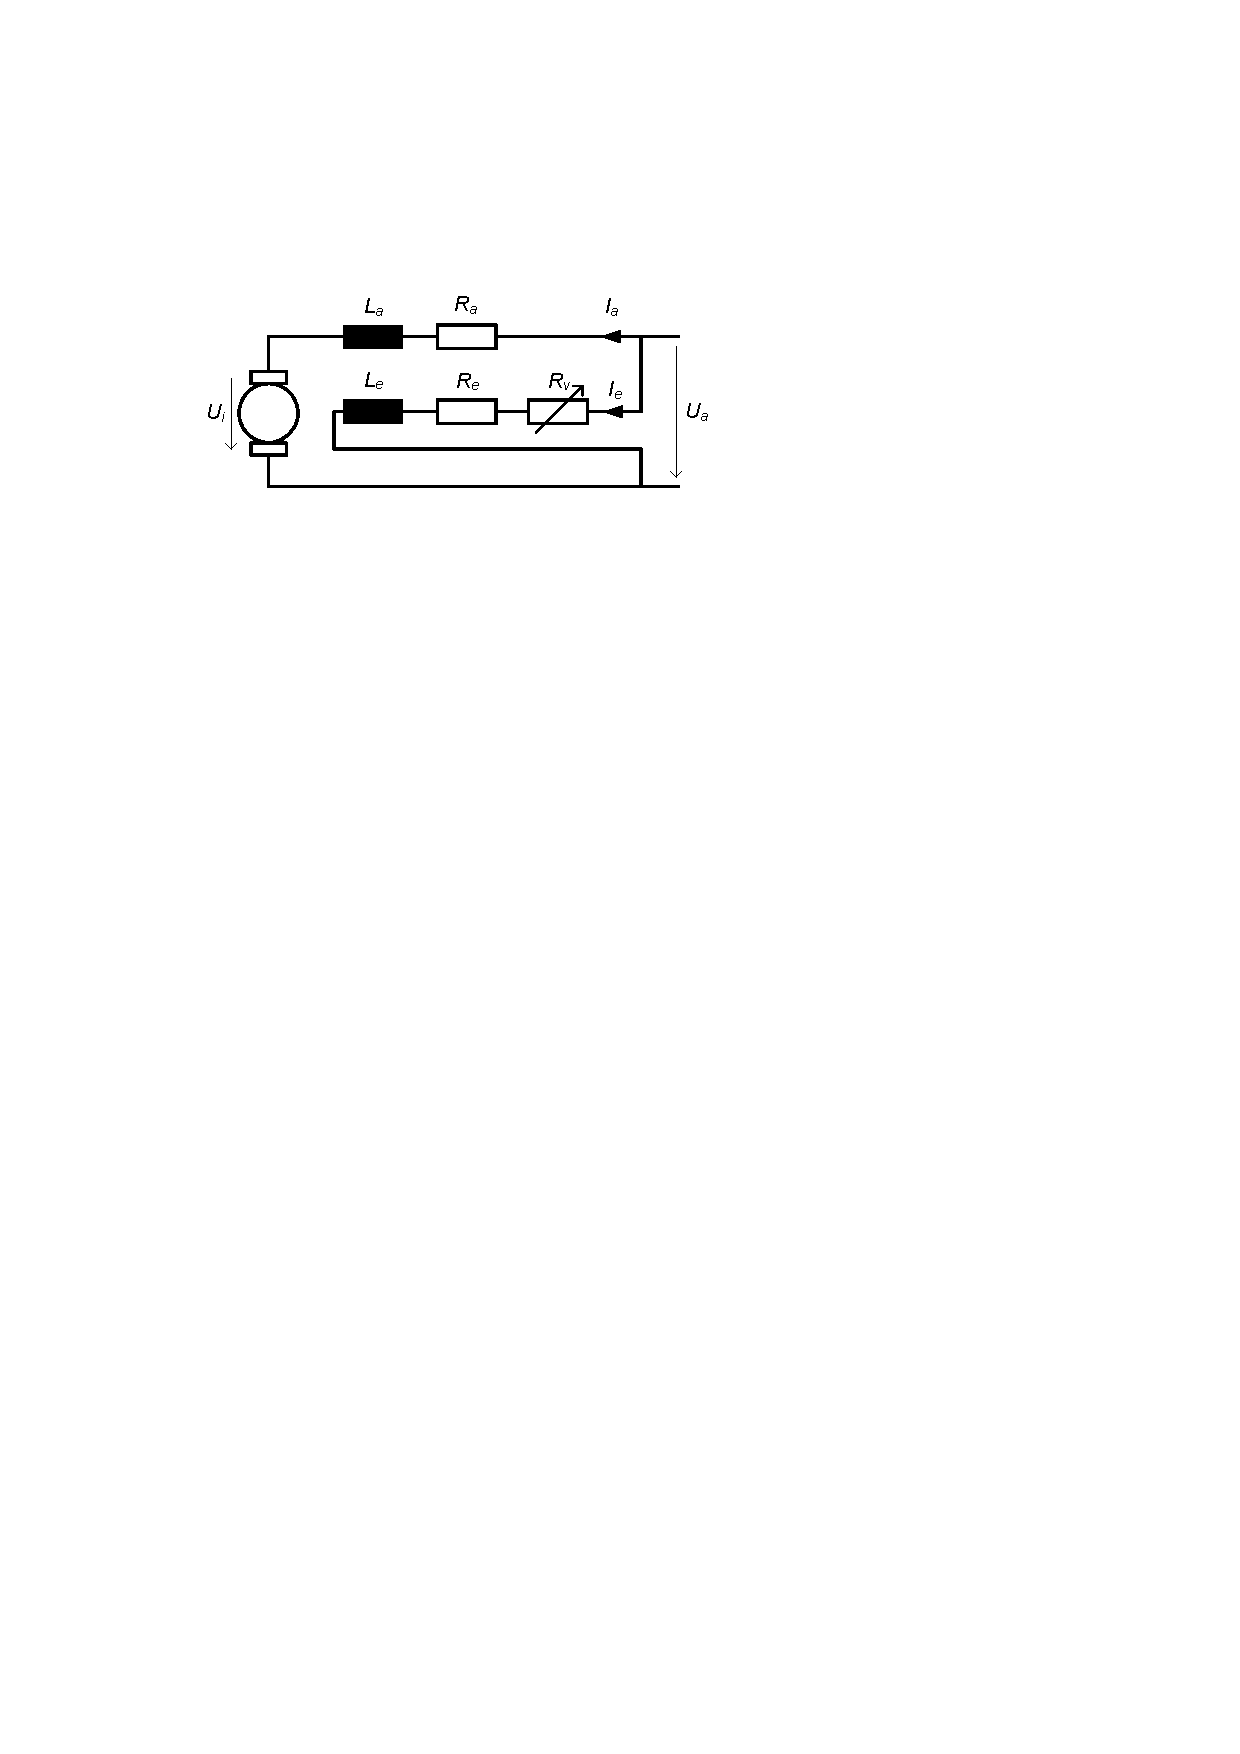
\includegraphics[width=0.6\columnwidth]{GM_N.pdf}

$\Phi = \frac{L_e}{N_e} \cdot I_e = \frac{L_e}{N_e} \cdot \frac{U_a}{R_e + R_V}$

Leerlaufdrehzahl: $w_{m0} = \frac{U_a}{c \Phi} = \frac{N_e (R_e + R_V)}{c \cdot L_e}$

Drehzahlabhänigkeit:\\ $w_m = \frac{N_e (R_e + R_V)}{c \cdot L_e} - \frac{R_a (R_e + R_V)^2 \cdot N_e^2}{(c \cdot L_e \cdot U_a)^2} \cdot M_{\ir el}$
\end{sectionbox}
\begin{sectionbox}
\subsection{Seriemaschine}
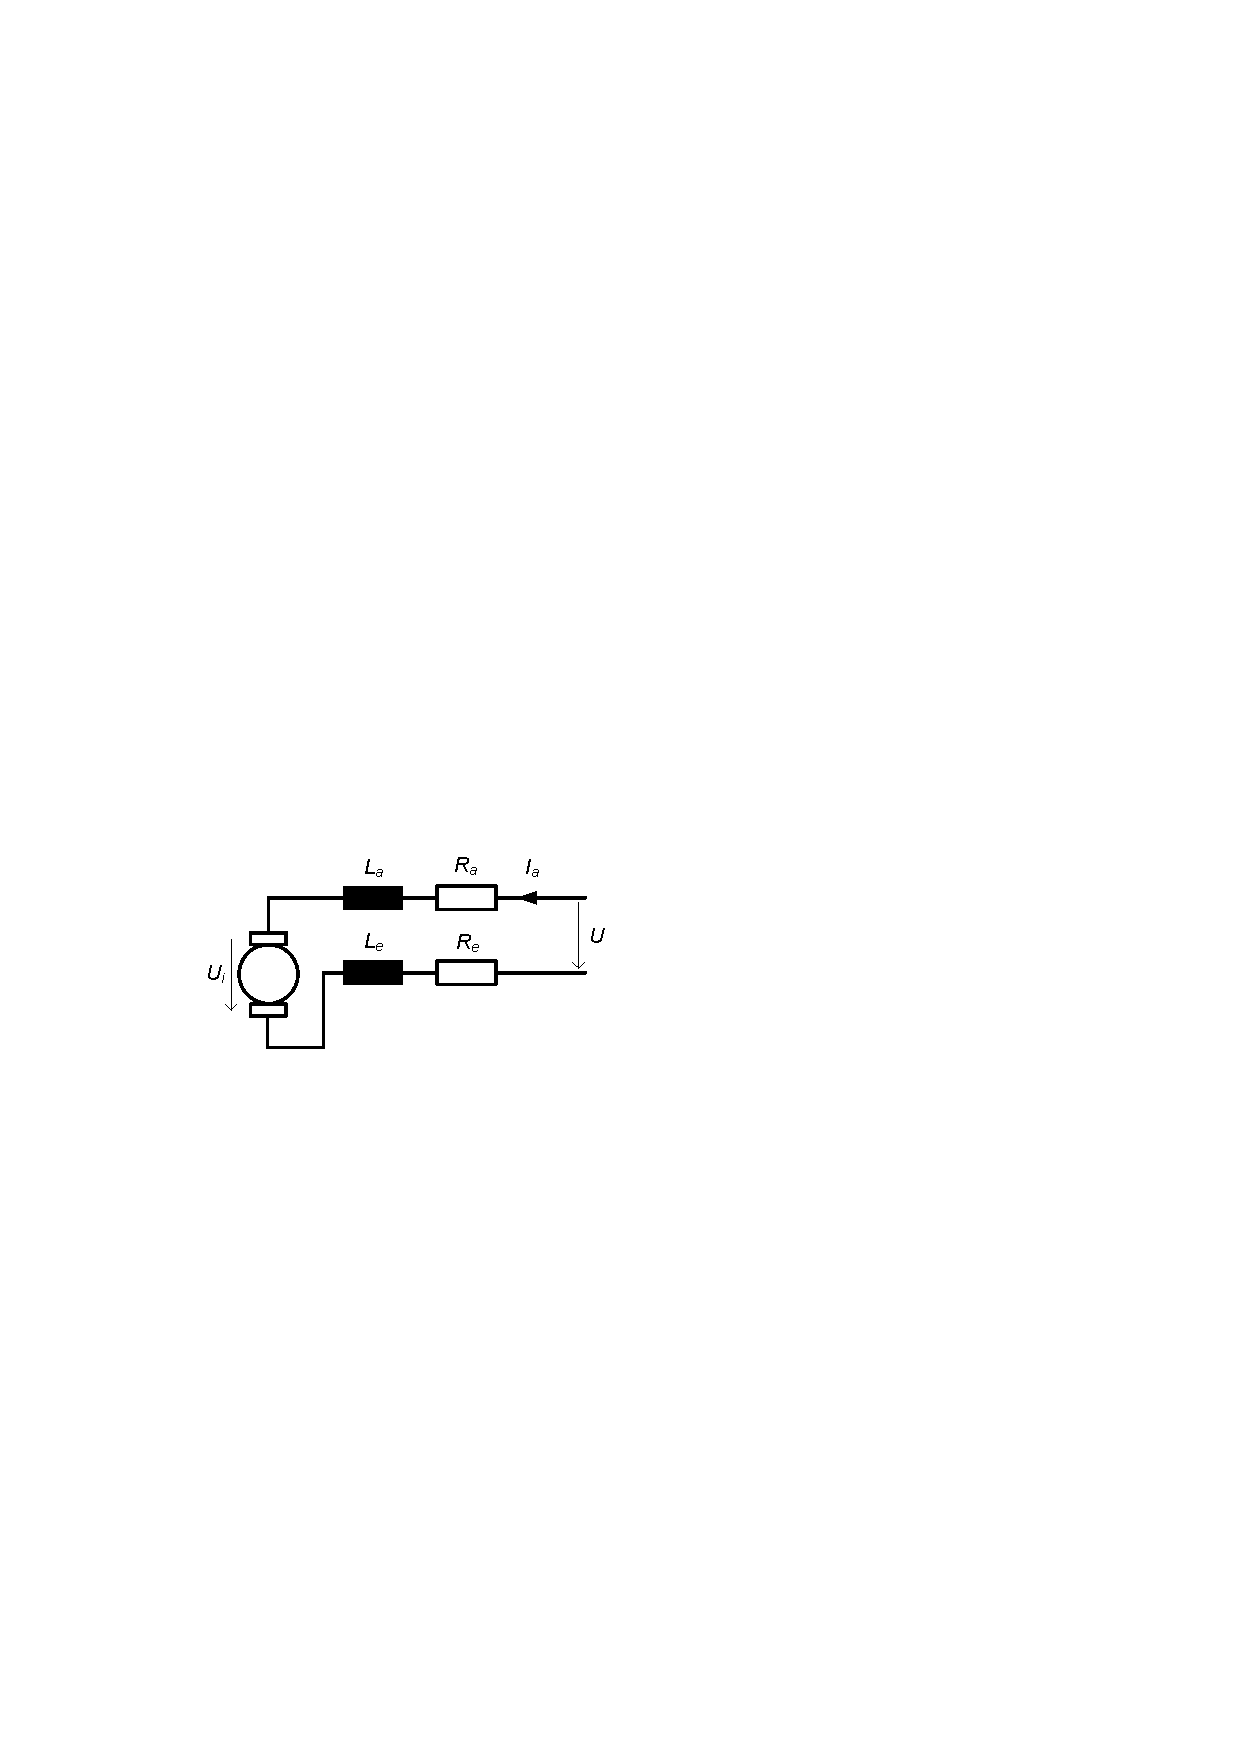
\includegraphics[width=0.6\columnwidth]{GM_S.pdf}

$I_e$ = $I_a$ = $I$

$\Phi = \frac{L_e}{N_e} \cdot I_e = \frac{L_e}{N_e} \cdot I_a$

$\omega_m = \frac{U- (R_a + R_e) I_a}{c \frac{L_e}{N_e} I_a}$

Drehmoment: $M = c \frac{L_e}{N_e} I_a^2 $

Ohne Last: $I_a \ra 0 \Ra \omega_m \ra \infty$
\end{sectionbox}

\section{Universalmotor}

\begin{sectionbox}
Gleichstrommaschine: Aber geblecht (wegen magnetischen Streufeldern)


Erregerspannung: $\vec U_e = \vec I \cdot R_e + \j \omega L_e \vec I$

Ankerspannung: $\vec U_a = \vec I \cdot R_a + \j \omega L_a \vec I$

$\vec U_i = c \vec \Phi_{\ir de} \omega_m$ \\


$\vec U = \vec U_i + \vec I (R_a + R_e) + \j \omega \vec I (L_a + L_e)$

$M_{\ir el} = c \Phi_{\ir de} I = c \frac{L_e}{N_e} I^2$

Drehzahlabhängigkeit:

$\omega_m = \frac{U- (R_a + R_e) \vec I - \j \omega (L_a + L_e) \vec I}{\sqrt{c \frac{L_e}{N_e}M_{\ir el}}}$ \\
$\omega_m \propto \frac{U_i}{\sqrt{M_{\ir el}}}$

Typische Auslegungen der Laufzeiten: Bohrmaschine ($50 \si{\hour}$)
\end{sectionbox}
\section{Drehfeldmaschinen}

\begin{sectionbox}
Rotierendes Feld. Beispiele: Synchronmaschine, Asynchronmaschine

Flussverkettung: $\vec \Psi_{\ir gesamt} = \frac{3}{2} \cdot \hat I \cdot L_{\ir ph} \cdot e^{\j ( \omega t + \varphi_i)}$

$\vec \Psi = \hat I \cdot L_{\ir ph} \cdot e^{\j (\omega t + \varphi_i)}$

Amplitude der Flussverkettungs-Zeiger entspricht der Amplitude der Phasengrößen (zur Normierung). \\

\subsection{Transformation Dreiphasen $\ra$ Drehzeiger}

$\vec x(t) = \frac{2}{3} \cdot \left[ x_a (t) + x_b (t) \cdot \e^{\j 120 \si{\degree}} + x_c (t) \cdot \e^{- \j 120 \si{\degree} } \right]$

mit
$e^{\j 120 \si{\degree}} = - \frac{1}{2} + \j \cdot \frac{\sqrt{3}}{2} $
\quad $e^{- \j 120 \si{\degree}} = - \frac{1}{2} - \j \cdot \frac{\sqrt{3}}{2} $ \\

In der komplexen Ebene: $\vec x (t)  = x_\alpha + \j x_\beta$

$x_\alpha  = \frac{1}{3} ( 2 x_a - x_b - x_c)$

$x_\beta = \frac{1}{\sqrt{3}} (x_b - x_c)$

Nullsystem (gleichphasige Komponenten):

$x_0 (t) = \frac{1}{3} \cdot \left[ x_a + x_b + x_c \right]$

\subsection{Drehzeiger $\ra$ (ruhende) Zeiger}

$\vec X(t) = \vec x (t) \cdot \e^{- \j \int \omega_K \diff t}$

Für konstante $\omega_K$ (Umlaufgeschwindigkeit des KS): $\vec X(t) = \vec x(t) \cdot \e^{- \j \omega_K t}$

\subsection{Zeiger $\ra$ Drehzeiger}

$\vec x(t) = \vec X (t) \cdot \e^{\j \omega_K t}$ 

\subsection{Drehzeiger $\ra$ Phasengrössen}
$x_a = x_\alpha + x_0$

$x_b = \frac{1}{2} ( \sqrt 3 x_\beta - x_\alpha ) + x_0$

$x_c = \frac{1}{2} (- \sqrt 3 x_\beta - x_\alpha ) + x_0$ 

\end{sectionbox}

\section{Synchronmaschine}

\begin{sectionbox}
Stator: Dreiphasige Wicklung

Rotor: Rotorwicklung (mit Gleichstrom über Schleifring) oder Permanentmagnet\\

\emph{Formeln gelten für Phasengrössen (Strom und Spannung)} \\

Polpaarzahl: $\omega_{\ir mech} = \omega_{D1} = \frac{\omega_1}{p}$ \quad $M = p \cdot M_{p}$ 

mit $M_p$: Drehmoment pro Polpaar 

$\Ra$ Leistung unabhängig von der Polpaarzahl\\

Polradspannung $\vec U_p = \j \omega_1 \vec \Psi_p$: \\

 $\abs{\vec U_p} = \omega_1 \abs{\vec \Psi_p}$\\


 $\vec U_1 = \vec U_p + \Delta \vec U$
 $\Delta \vec U = \j X_d \cdot \vec I_1 (+ R \cdot \vec I_1)$ \\

Polradwinkel $\theta$: Winkel zwischen Stator $\vec U$ und Polradspannung $\vec U_p$:

$\theta > 0 \ra$ motorischer Betrieb, $\theta < 0 $ generatorischer Betrieb \\


Leistung:

 $P = \Re{\vec S}  = \Re{ 3 \vec U \vec I^* } = \Re{3( U_d + \j U_q ) (I_d - \j I_q)}$ \\ $= 3 (U_d I_d + U_q I_q)$ \\

 d := direct (in Flussrichtung)

 $U_{1q} = \abs{\vec U_1} \cos \theta$

 $U_{1d} = - \abs{\vec U_1} \sin \theta$

 \end{sectionbox}

\begin{sectionbox}
\subsection{Schenkelpolmaschine}
kurzer Rotor, grosser Druchmesser; Stator geblecht, Rotor aus Eisen

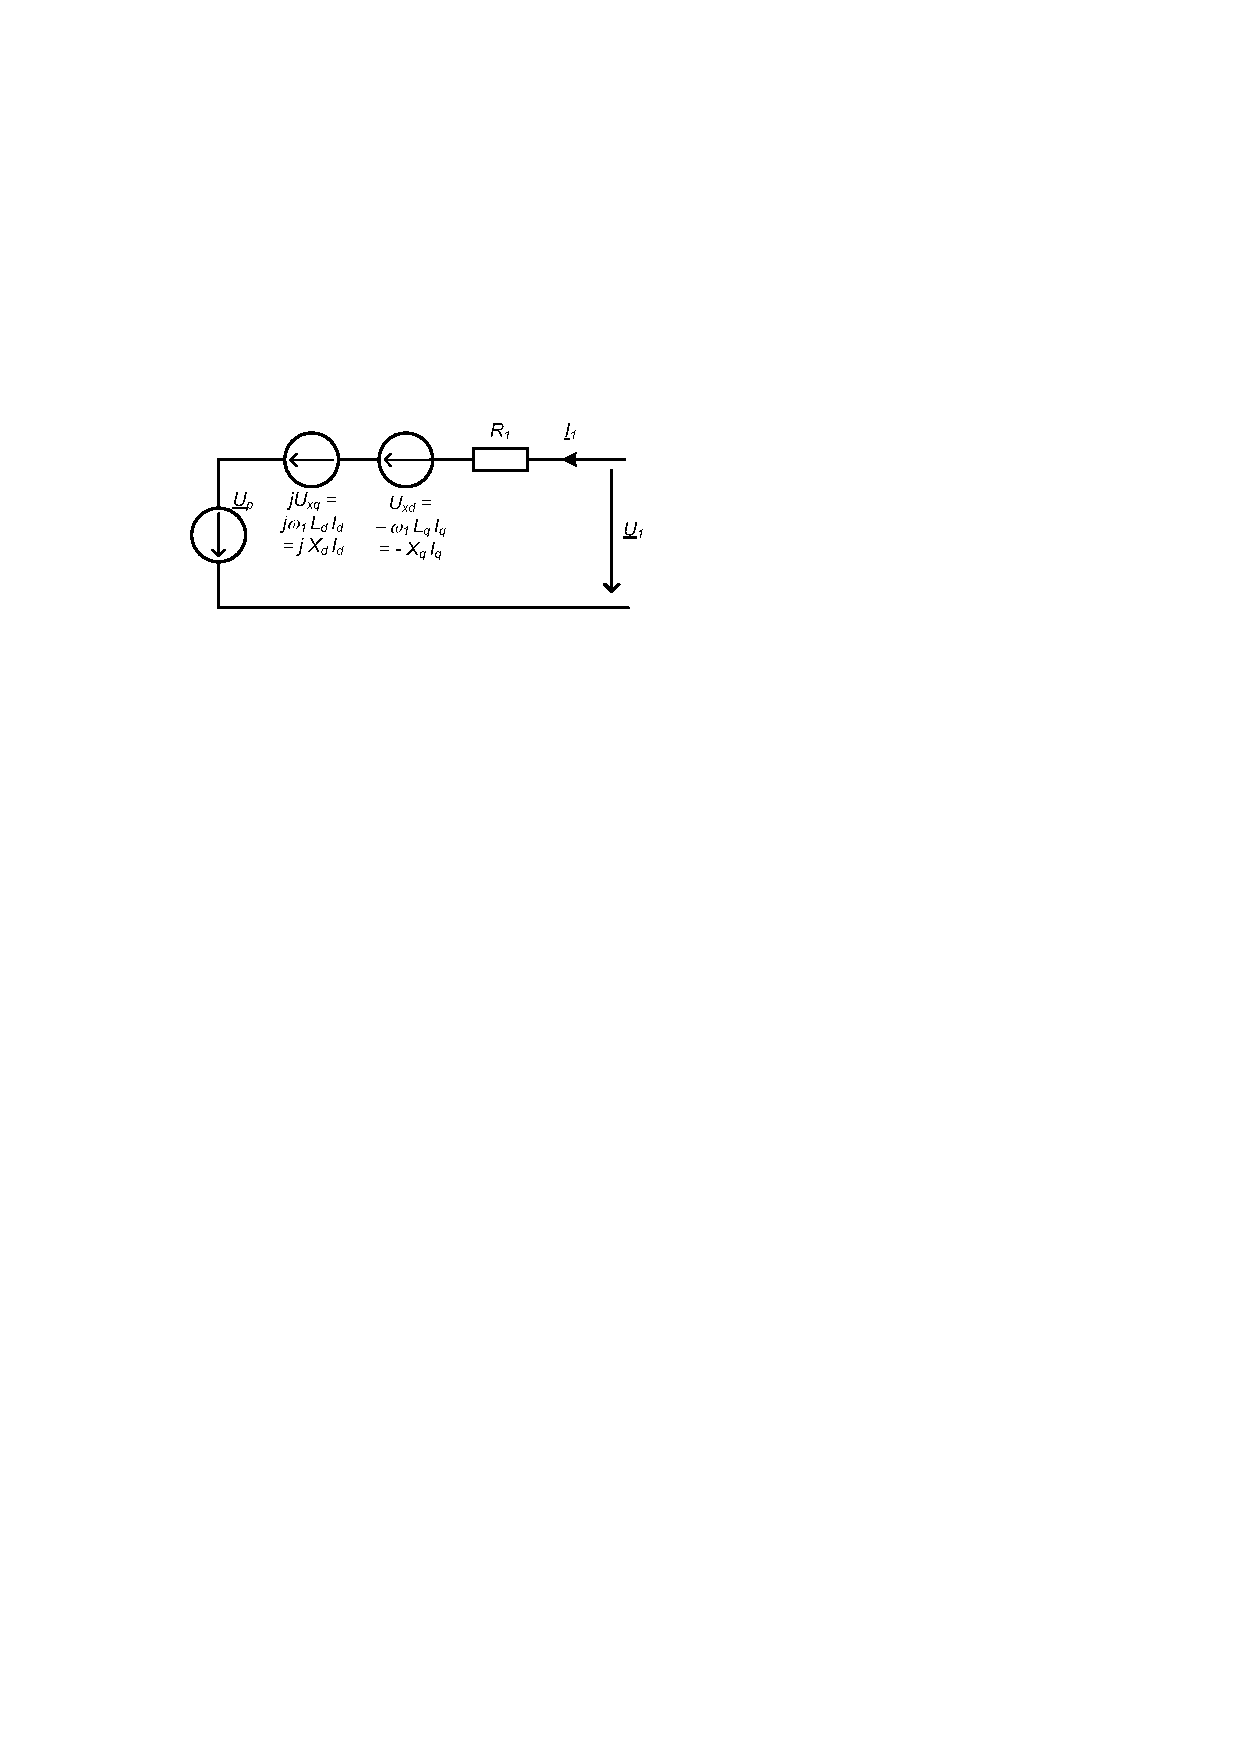
\includegraphics[width=0.7\columnwidth]{SM_SP.pdf}

Statorspannung:

$\vec U_1 = \vec I_1 R_1 + U_{xd} + \j U_{xq} + \j U_P = \vec I_1 R_1 - \omega_1 L_q I_q + \j \omega_1 L_d I_d + \j U_P$

Stromkomponenten:

$I_{1d} = \frac{U_1 X_q \cos \theta - U_1 R_1 \sin \theta - U_P X_q}{R_1^2 + X_d X_q}$

$I_{1q} = \frac{U_1 \sin \theta + R_1 I_{1d}}{X_q} = \frac{U_1 R_1 \cos \theta + U_1 X_d \sin \theta - U_P R_1}{R_1^2 + X_d X_q}$ 

Leistung:
 $P_m = M \omega_{\ir mech}$

Moment: 

$M = \frac{3 U_1 U_P}{\omega_{\ir mech} X_d} \sin (\theta ) + \frac{3 U_1^2}{2 \omega_{\ir mech}} (\frac{1}{X_q} - \frac{1}{X_d} ) \sin ( 2 \theta )$
\end{sectionbox}

\begin{sectionbox}
 \subsection{Vollpolmaschine}

 langer Rotor, kleiner Durchmesser; 
für schnelllaufende Maschinen, Turbogenerator

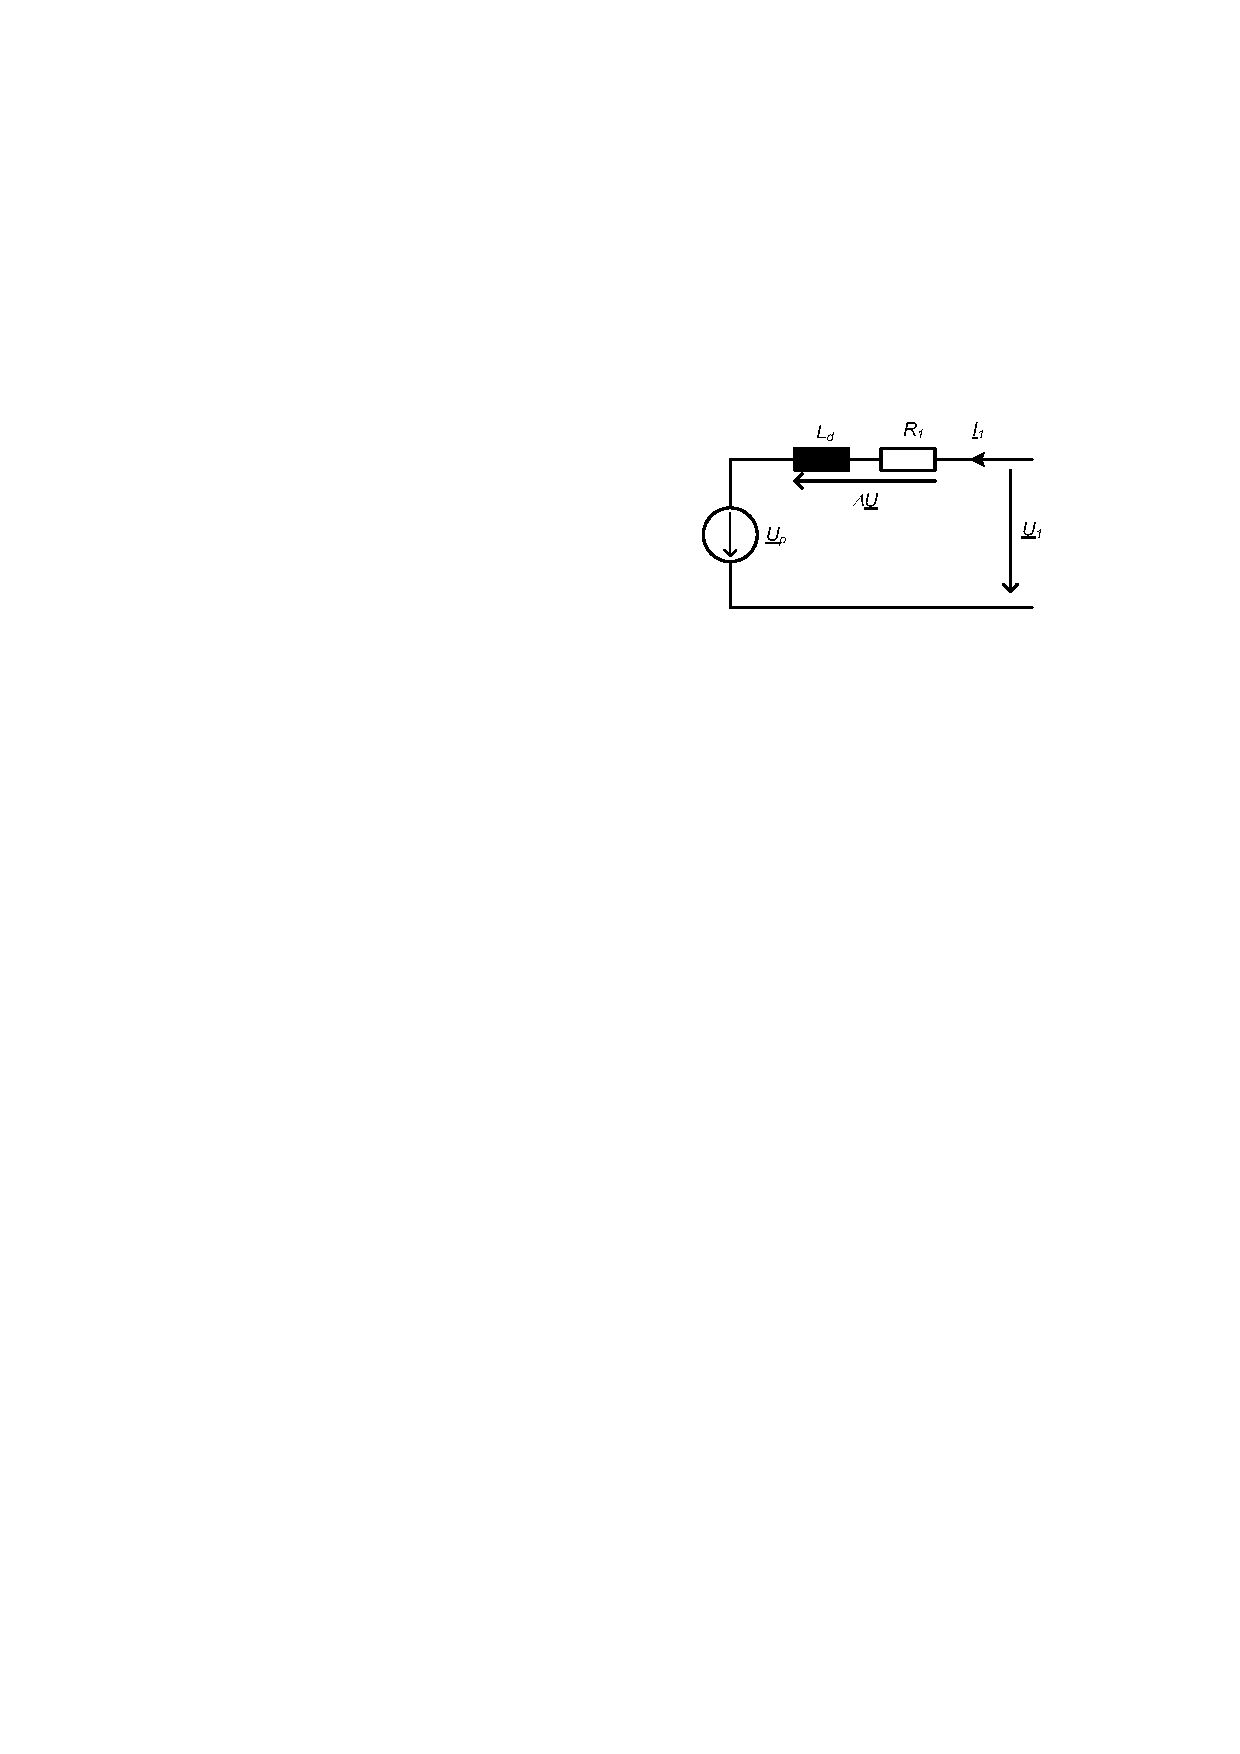
\includegraphics[width=0.5\columnwidth]{SM_VP.pdf}


Statorspannung:
$\vec U_1 = \vec I_1 (R_1 + \j \omega_1 L_d) + \j U_P$

Leistung:
 $P_m = M \omega_{\ir mech}$

Moment: 
$M = \frac{3 U_1 U_P}{\omega_{\ir mech} X_d} \sin ( \theta ) $
\end{sectionbox}

\begin{sectionbox}
\subsection{SM am Netz} 
Zeigerlängen entsprechen den Effektivwerten der Phasengrößen! \\

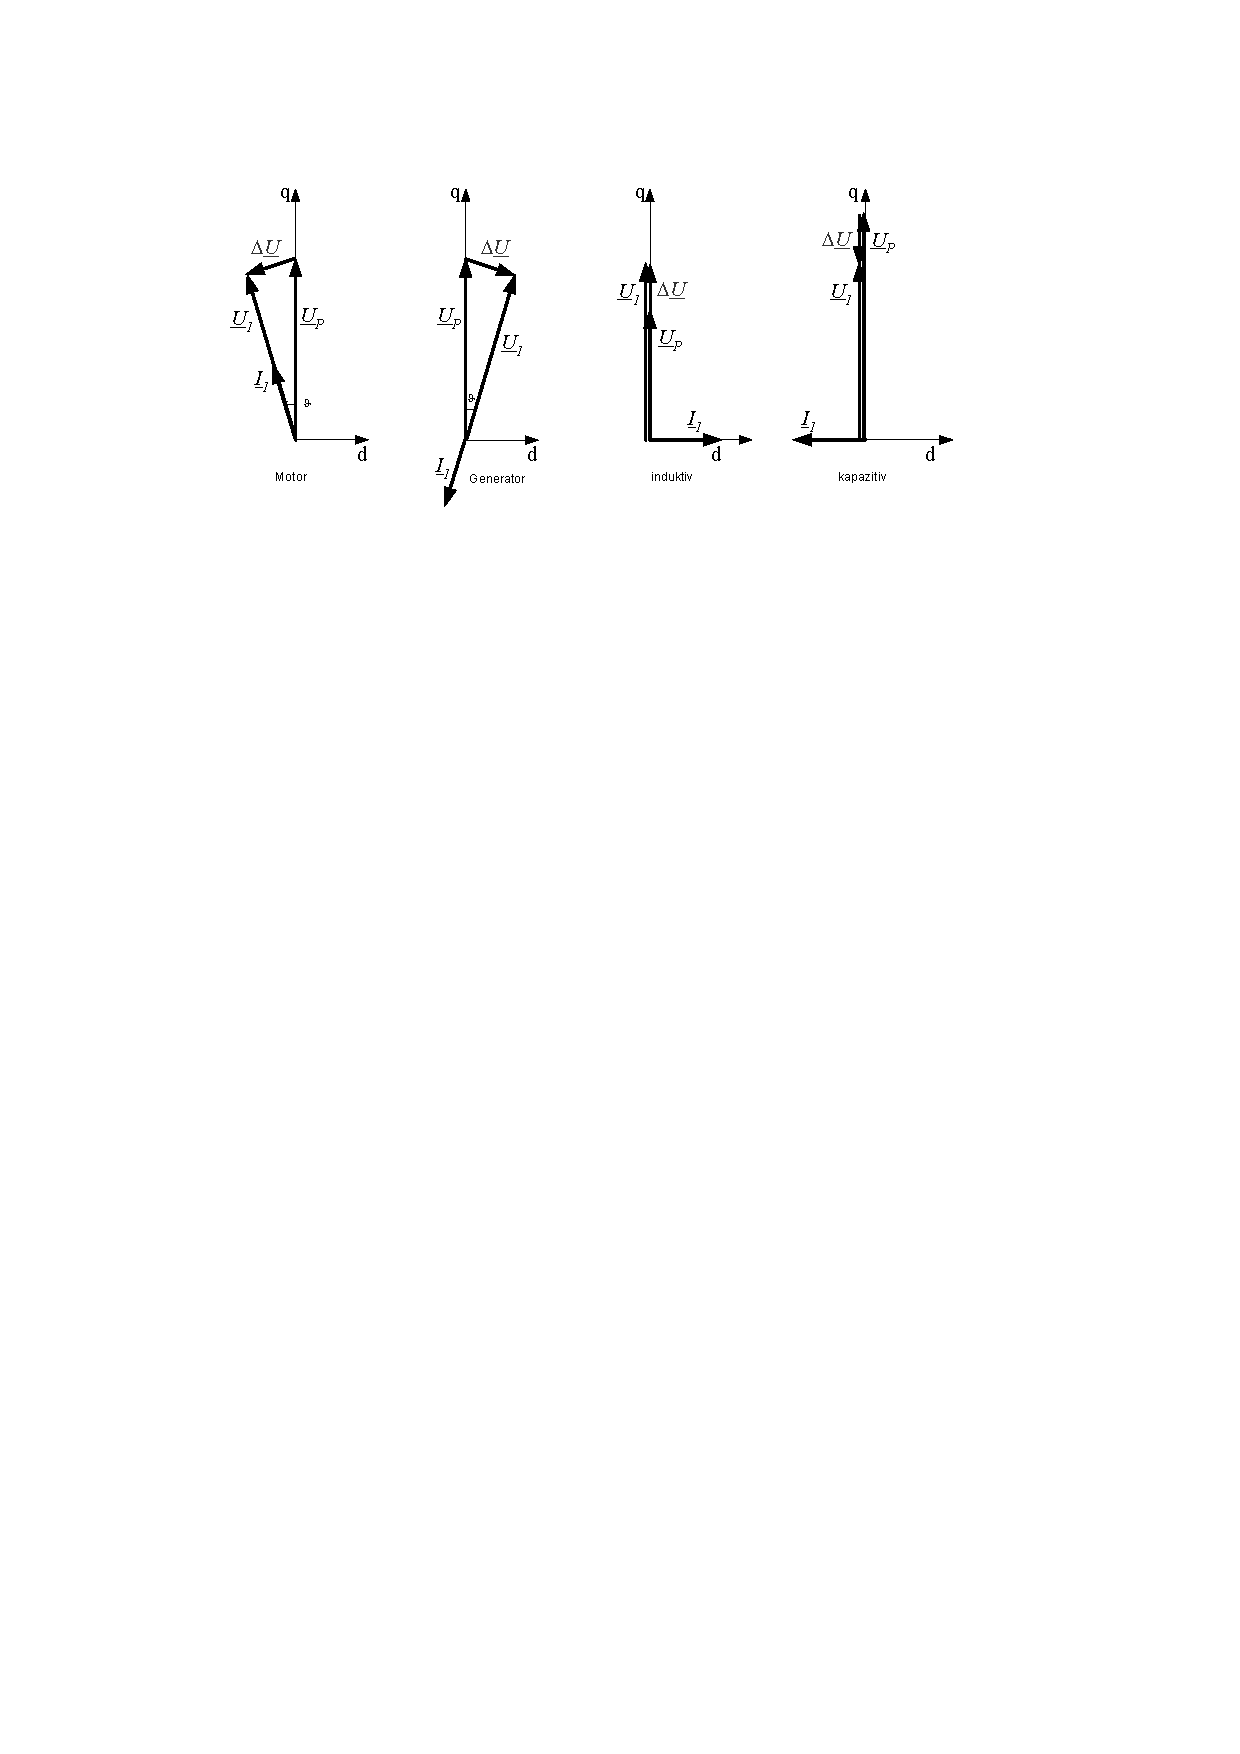
\includegraphics[width=\columnwidth]{SM_RZ.pdf}

\end{sectionbox}
\begin{sectionbox}
\subsection{Raumzeigerdarstellung}
Zeigerlängen entsprechen den Amplituden der Phasengrößen! \\

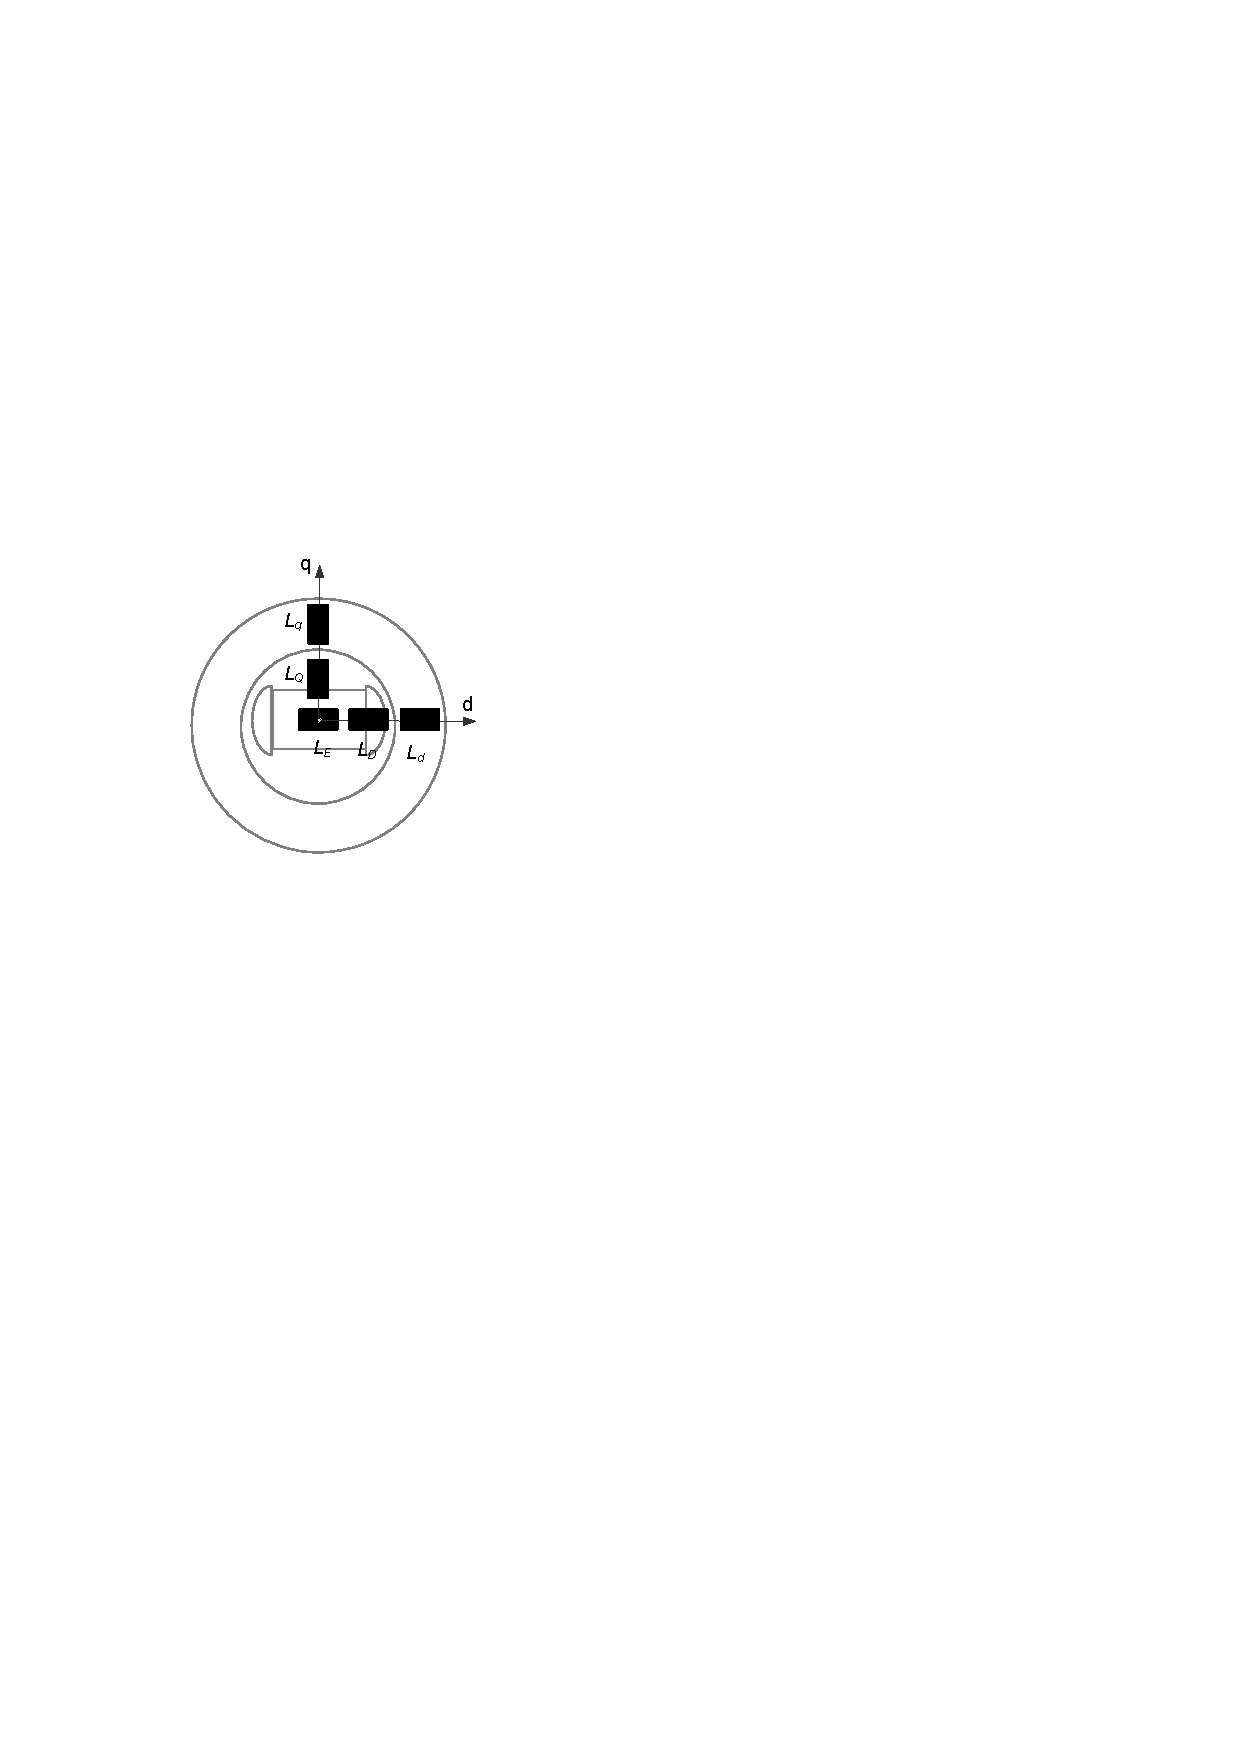
\includegraphics[width=0.4\columnwidth]{SM_RZ2.pdf}

In Verbraucherzählpfeilsystem: \\ \\
Statorspannung:\\
$U_d = R_1 I_d + \frac{\diff \Psi_d}{\diff t} - p \omega_{\ir mech} \Psi_q$\\
$U_q = R_1 I_q + \frac{\diff \Psi_q}{\diff t} + p \omega_{\ir mech} \Psi_d$

Statorfluss: \\
$\Psi_d = L_d I_d + L_{dE} I_E + L_{dD} I_D$ \\
$\Psi_q = L_q I_q +  L_{qQ} I_Q$


Dämpferspannung:

$0 = R_D I_D + \frac{\diff \Psi_D}{\diff t}$ \\
$0 = R_Q I_Q + \frac{\diff \Psi_Q}{\diff t}$

Dämpferfluss:

$\Psi_D = L_{dD} I_d + L_{ED} I_E + L_D I_D$ \\
$\Psi_Q = L_{qQ} I_q + L_{Q} I_{Q}$

Erregerspannung:
$U_E = R_E I_E + \frac{\diff \Psi_E}{\diff t}$

Erregerfluss:
$\Psi_E = L_{dE} I_d + L_E I_E + L_{ED} I_D$

Drehmoment:

$M = \frac{3 p}{2} (I_q \Psi_d - I_d \Psi_q)$

Drehzahl:

$\omega_{\ir mech} = \frac{1}{J} \int (M- M_{\ir Last}) \diff t$

 
 \end{sectionbox} 

 \section{Asynchronmaschine}
\label{sec:async}
 \begin{sectionbox}
\ctikzset{bipoles/length=3em}
 \begin{circuitikz}[scale = 0.8] \draw
 (0,0) to[short, o-, i=$I_1$] (1,0) to[R, l=$R_1$] (2,0) to [L, l=$L_{\sigma 1}$] (3,0) -- (3,0)
 (3,0) to[L, l=$L'_{\sigma2}$] (4,0) to[R, l=$R'_2$] (5,0) to[R, l=$R'_S$] (6,0) to[short, i<=$I'_2$, , -o] (7,0 )
 (3,0) -- (3, -0.6) -- (2.5, -0.6) to[L, l=$L_h$] (2.5, -2.3) --  (3, -2.3)
 (3, -0.6) -- (3.5, -0.6) to[R, l=$R_{\ir Fe}$] (3.5, -2.3) --  (3, -2.3) -- (3, -3)
 (0,-3) to[short, o-o] (7,-3)
 (0,0) to[open, v=$U_1$] (0,-3)
 (7,0) to[open, v^=$U'_2 / s$] (7,-3)
  (2,0) to[open, v=$U_{h1} $] (2,-3)
   (4.3,0) to[open, v^=$U'_{h2}$] (4.3,-3);
 \end{circuitikz}
\begin{symbolbox}
\begin{tabular}{rl}
$\omega_{D1}$ & Frequenz des Statordrehfeldes \\
$\omega_1$ & Statorfrequenz \\
$\omega_{D2}$ & Frequenz des Rotordrehfeldes (relative Rotorfrequenz)\\
$\omega_2$ & Rotorfrequenz \\
$\omega_{\ir mech}$ & mech. Drehkreisfrequenz \\ 
\end{tabular}
\end{symbolbox}

 Statordrehfeld: $\omega_{D1} = \frac{\omega_{1}}{p}$ 

 Drehfeld des Rotors: $\omega_{D2} = \omega_{D1} - \omega_{\ir mech}$

$\omega_2 = p \cdot \omega_{D2}$

$\omega_2 = \omega_1 - p \cdot \omega_{\ir mech}$ \\

Schlupf

$s = \frac{n_{\ir syn} - n}{n_{\ir syn}} = \frac{\omega_1 - p \cdot \omega_{\ir mech}}{\omega_1} = \frac{\omega_2}{\omega_1}$ 

$\omega_2 = s \cdot \omega_1$

\end{sectionbox}
\begin{sectionbox}
\subsection{Spezialfälle}

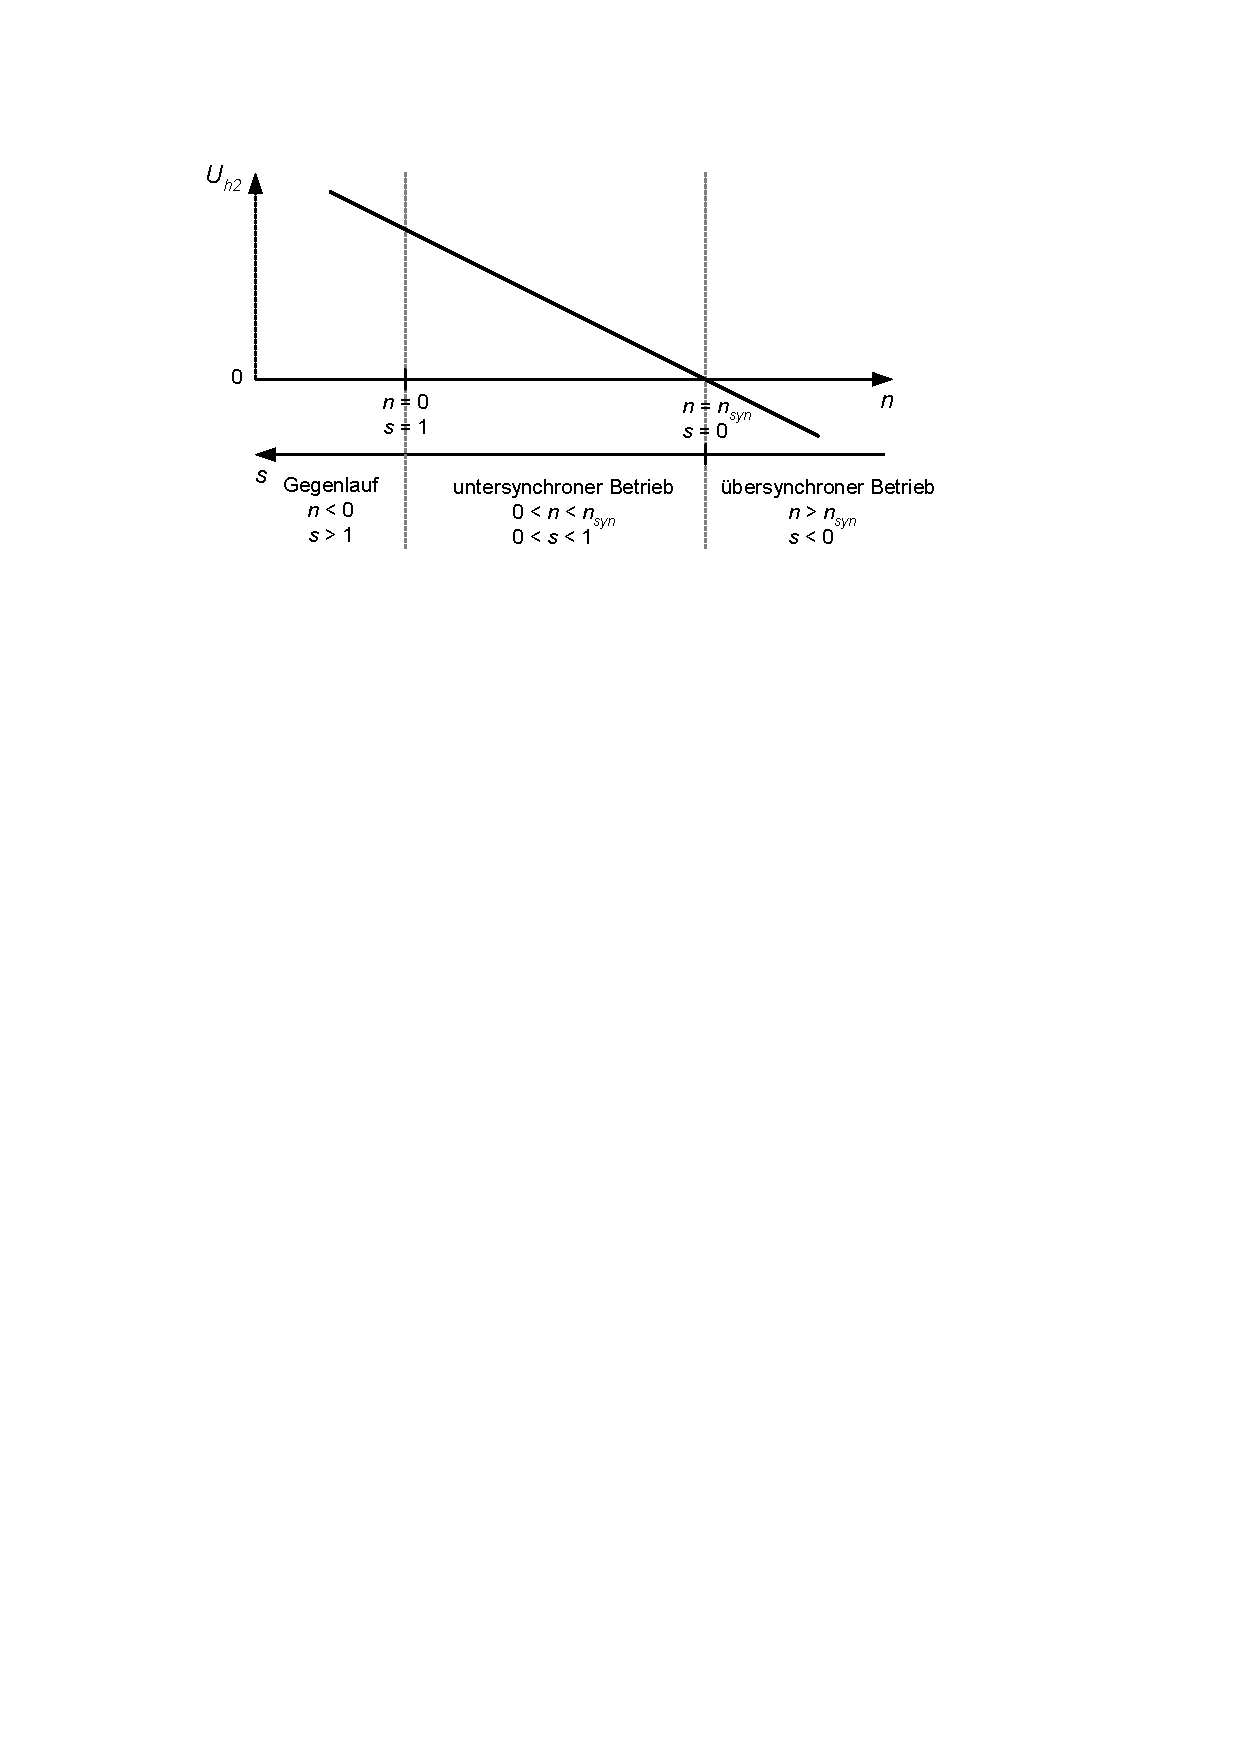
\includegraphics[width=0.9\columnwidth]{ASM_Betrieb.pdf}

\subsection{Stillstand}

$n = 0$
\quad $s = 1$
\quad
$\omega_2 = \omega_1$
\quad
$U_{h2} = \frac{U_{h1}}{\text{ü}}$ 

\subsection{Synchrondrehzahl}


$n = n_{\ir syn}$
\quad $s = 0$
\quad
$\omega_2 = 0$
\quad
$U_{h2} = 0$ 

 \subsection{Leerlauf}
  $\omega_{D2} = 0 \ra \omega_{\ir mech} = \omega_{\ir syn} = \omega_{D1} = \omega_1 /p $ 

  Im Leerlauf ist der Schlupf 0 $s = 0$

\end{sectionbox}
\begin{sectionbox}
\subsection{Leistungen}

Rotorleistung: $P_2 = 3 \cdot U_{h2} \cdot I_2$

Statorleistung: $P_1 = P_\delta = 3 \cdot U_{h1} \cdot I_1$

Luftspaltleistung: $P_\delta = P_1 - 3 \cdot R_1 \cdot I_1^2 - P_{\ir Fe}$ 

$P_2 = s \cdot P_\delta$ \quad $P_\delta = P_2 + P_{\ir mech}$

\end{sectionbox}
\begin{sectionbox}
\subsection{Wirkungsgrad}
Motorbetrieb: $\eta = \frac{P_{\ir mech}}{P_1} < \frac{P_{\ir mech}}{P_\delta} = 1 - s$ \quad $0 < s < 1$

Generatorbetrieb: $\eta = \frac{P_1}{P_{\ir mech}} <\frac{P_\delta}{P_{\ir mech}} = \frac{1}{1 -s }$ \quad $s < 0$
\end{sectionbox}


\begin{sectionbox}
\subsection{Läuferwiderstand $R_S$}

$R_2 + R_S = \frac{R_2}{s}$

$R_S = R_2 \cdot \frac{1 - s}{s}$ 
\end{sectionbox}

\begin{sectionbox}
\subsection{Drehmoment}

$M_{\ir el} = \frac{P_{\ir mech}}{\omega_{\ir mech}} = \frac{P_\delta}{\omega_{D1}} = \frac{P_\delta \cdot p}{\omega_1} = \frac{3 p }{\omega_1} \cdot \frac{U_{h20}^2}{\left(\frac{R_2}{s}\right)^2 + (\omega_1 L_{2 \sigma})^2} \cdot \frac{R_2}{s}$

Linearer Bereich: $M_{\ir el} = \frac{3 \cdot p}{\omega_1} \cdot \frac{U_1^2}{R_2'} \cdot s$

Kippschlupf: $s_k = \frac{R_2'}{\sqrt{R_1^2 + (\omega_1 L_{1 \sigma} + \omega_1 L_{2 \sigma}')^2}}$

Kippmoment: $M_k = \frac{3p}{2 \omega_1} \cdot \frac{U_1^2}{(R_1 + \omega_1 L_{1 \sigma + \omega_1 L_{2 \sigma}'})}$

Kloss'sche Gleichung: $\frac{M_{\ir el}}{M_k} = \frac{2}{\frac{s}{s_k} + \frac{s_k}{s}}$
\end{sectionbox}

\begin{sectionbox}
\subsection{Stillstehendes Koordinatensystem}

Statorspannungsgleichung:

$\vec u_1 = R_1 \vec i_1 + \frac{\diff \vec \Psi_1}{\diff t}$ 

Rotorspannungsgleichung: 

$\vec u_2 = R_2 \vec i_2 + \frac{\diff \vec \Psi_2}{\diff t}  \j p \omega_{\ir mech} \vec \Psi_2$

Flussverkettungen: 

$\vec \Psi_1 = L_1 \vec i_1 + L_h \vec i_2$

$\vec \Psi_2  = L_2 \vec i_2 + L_h \vec i_1$


Drehmoment:

$M = \frac{3p}{2} \Im{\vec \Psi_1^* \vec i_1} = \frac{3p}{2} \frac{L_h}{L_2} \Im{\vec \Psi_2^* \vec i_1} = $ \\ $ = \frac{3p}{2} \frac{L_h}{L_1} \Im{\vec \Psi_1^* \vec i_2} $ 

Mechanische Drehzahl: 

$\omega_{\ir mech} = \frac{1}{J} \int (M - M_{\ir Last}) \diff t$ \\

Flussverkettung (allg.): $\Psi = L \cdot i = N \cdot \Phi$
\end{sectionbox}

\begin{sectionbox}
  \subsection{Rotierendes Koordinatensystem}

Statorspannungsgleichung:

  $\vec u_1 = R_1 \vec i_1 + \frac{\diff \vec \Psi_1}{\diff t} + \j \omega_K \vec \Psi_1$

Rotorspannungsgleichung:

  $\vec u_2 = R_2 \vec i_2 + \frac{\diff \vec \Psi_2}{\diff t} + \j (\omega_K - p \omega_{\ir mech} ) \vec \Psi_2$


Statorfluss:

  $\Psi_1 = L_1 \vec i_1 + L_h \vec i_2$

Rotorfluss:

  $\Psi_2 = L_2 \vec i_2 + L_h \vec i_1$

Drehmoment:

  $M = \frac{3 p}{2} \Im{\vec \Psi_1^* \vec i_1} = \frac{3p}{2} \frac{L_h}{L_2} \Im{\vec \Psi_1^* \vec i_1}$ \\$ =  \frac{3p}{2} \frac{L_h}{L_1} \Im{\vec \Psi_1^* \vec i_2} $

  $\omega_{\ir mech} = \frac{1}{J} \int (M - M_{\ir Last}) \diff t$

$R_S = R_2 \cdot \frac{1 -s }{s}$

 \end{sectionbox}

 \section{Umrichter}

 \begin{sectionbox}
 \subsection{B2}
$U_{\ir di0} = \frac{1}{T} \int \limits_0^T u_d \cdot \diff t = \frac{1}{\pi} \int \limits_0^\pi u_d \cdot \diff (\omega t) = \frac{2 \sqrt 2}{\pi} U_N = 0.900 U_N$
 
\subsubsection{Gesteuert}
Mittelwert der Ausgangsspannung in Abhängigkeit des Zündwinkels $\alpha$:

$U_{\ir di \alpha} = \frac{1}{\pi} \int \limits_\alpha^{\alpha + \pi} u_d \cdot \diff (\omega t) = U_{di 0} \cdot \cos \alpha$ 
 \subsection{B6}
 Idealisierte DC-Spannung (Mittelwert): 

$U_{\ir di0} = \frac{3 \sqrt 2}{\pi} \cdot U_N = 1.35 U_N$

Effektivwert des Netzstromes:

$i_{N, \ir eff} = \sqrt{\frac{2}{3}} I_d $

Halbleiterstrom:

Effektivwert: $i_{\ir HL, eff} = \sqrt{\frac{1}{3}} I_d$

Mittelwert: $i_{\ir HL,  avg} = \frac{1}{3} I_d$

\subsubsection{Gesteuert}

$U_{\ir di \alpha} = U_{\ir di0} \cdot \cos \alpha$

Leistungsfaktor: $\lambda = 0.955 \cdot \cos \alpha$
 \end{sectionbox}

 \section{Halbleiter}
\begin{sectionbox}

 \begin{tablebox}{lll}
 & $25 \si{\celsius} (\text{ca. } 300 \si{\kelvin})$ & $125 \si{\celsius} (
 \text{ca.  } 400 \si{\kelvin})$ \\ 
\cmrule
 $n_{io}$ & $1.5 \cdot 10^{10} \si{1\per \centi \meter^3}$ & $10^{13} \si{1 \per \centi \meter^3}$ \\
 $\rho$ & $2.5 \cdot 10^5 \si{\ohm \centi \meter}$ &$3.5 \cdot 10^2 \si{\ohm \centi \meter}$
 \end{tablebox}
\begin{symbolbox}
\begin{tabular}{cc}
$n_{io}$ & Dichte der freien Elektronen im Leitungsband \\
$p_{io}$ & Dichte der freien Löcher im Valenzband \\
$k$ & Boltzmann Konstante \\
$E_{\ir Fi}$ & Fermi-Niveau (Energieniveau mit $W_{\ir FD} (E_{\ir Fi})= 0.5$)
\end{tabular}
\end{symbolbox}

Fermi-Dirac Funktion:

$W_{\ir FD} (E) = \frac{1}{1 + \exp\left(\frac{E-E_{\ir Fi}}{k \cdot T}\right)}$

gibt die Besetzungswahrscheinlichkeit eines Energiezustandes im idealen Elektronengas an.

Bewegungsgleichung für Elektronen:

$m \cdot \left(\frac{\diff v}{\diff t} + \omega_0 \cdot v \right) = F_A = - e_0 \cdot E$
\begin{symbolbox}
\begin{tabular}{cc}
$m$ & effektive Masse \\
$\omega_0$ & Reibungskoeffizient \\
$v$ & Driftgeschwindigkeit \\
$F_A$ & Äussere Kraft \\
$e_0$ & Ladung \\
$E$ & Elektrische Feldstärke
\end{tabular}
\end{symbolbox}

Stationäre Geschwindigkeit der Ladungsträger:
$v = - \frac{e_0}{m \cdot \omega_0} \cdot E = \mu \cdot E$

Elektrische Leitfähigkeit:
$\sigma = e_0 (n \mu_n + p \mu_p)$

\begin{symbolbox}
\begin{tabular}{cc}
$n$ & Konzentration der freien Elektronen \\
$p$ & Konzentration der freien Löcher \\
$\mu_n$ & Beweglichkeit der freien Elektronen \\
$\mu_p$ & Beweglichkeit der freien Löcher \\
$n_i$ & Intrinsische Ladungsträgerdichte
 \end{tabular}
\end{symbolbox}

Ladungsträgerdichte im intrinsischen Halbleiter:
 $n_i^2 = n \cdot p$
\end{sectionbox}
\begin{sectionbox}
 \subsection{n-Dotierung}
 Dotierung mit Donatoren (Elektronen) $\Ra$ Elektronenleitung \\

Anhebung des Ferminiveaus $\Ra$ mehr Ladungsträger im Leitungsband

Dichte der freien Elektronen: $n_{n0} = p_{n0} + N_D^+$ \\
mit $p_{n0}$ verursacht durch Eigenleitung \\

Dichte der freien Löcher: $p_{n0} \approx \frac{n_i^2}{N_D^+}$

Elektrische Leitfähigkeit: $\sigma = e_0 \cdot N_D^+ \cdot \mu_n$
\end{sectionbox}
\begin{sectionbox}

 \subsection{p-Dotierung}
Dotierung mit Akzeptoren (Löchern) $\Ra$ Löcherleitung \\

Absenkung des Ferminiveaus $\Ra$ mehr Ladungsträger im Valenzband

Dichte der freien Elektronen: $p_{p0} = n_{p0} + N_A^-$ \\
mit $n_{p0}$ verursacht durch Eigenleitung \\

Dichte der freien Löcher: $n_{p0} \approx \frac{n_i^2}{N_A^-}$

Elektrische Leitfähigkeit: $\sigma = e_0 \cdot N_A^- \cdot \mu_p$

\end{sectionbox}
\begin{sectionbox}

\subsection{pn-Übergang}

Diffusionsgleichungen: \\
$i_{n, \ir Diff} = \epsilon_0 \cdot D_n \cdot \frac{\diff n}{\diff x}$\\
$i_{p, \ir Diff} = \epsilon_0 \cdot D_p \cdot \frac{\diff p}{\diff x}$

Diffusionskonstanten: 
$D_n = \mu_n \frac{k \cdot T}{\epsilon_0}$ \quad $D_p = \mu_p \frac{k \cdot T}{\epsilon_0}$

Poissongleichung: \\
 $\frac{\diff^2 V}{\diff x^2} = - \frac{\diff E}{\diff x} = - \frac{\rho}{\epsilon} = \frac{e_0}{\epsilon} \cdot \left[ n(x) - p(x)  N_D^+ (x) + N_A^- (x) \right]$

 Stromdichte-Gleichgewicht: \\
 $i_p (x) = e_0 \cdot \mu_p \cdot p \cdot E - \epsilon_0 \cdot D_p \cdot \frac{\diff p}{\diff x}$ \\
  $i_n (x) = e_0 \cdot \mu_n \cdot n \cdot E - \epsilon_0 \cdot D_n \cdot \frac{\diff n}{\diff x}$
\end{sectionbox}

\begin{sectionbox}
\subsection{Technologiekurve}
\end{sectionbox}

\section{Leistungshalbleiter}

\begin{sectionbox}
\subsection{Leistungsdiode}
Schaltsymbol: \\
 \begin{circuitikz}
\draw (0,0) to[D*] (1,0);
\end{circuitikz}
\end{sectionbox}

\begin{sectionbox}
\subsubsection*{Struktur}
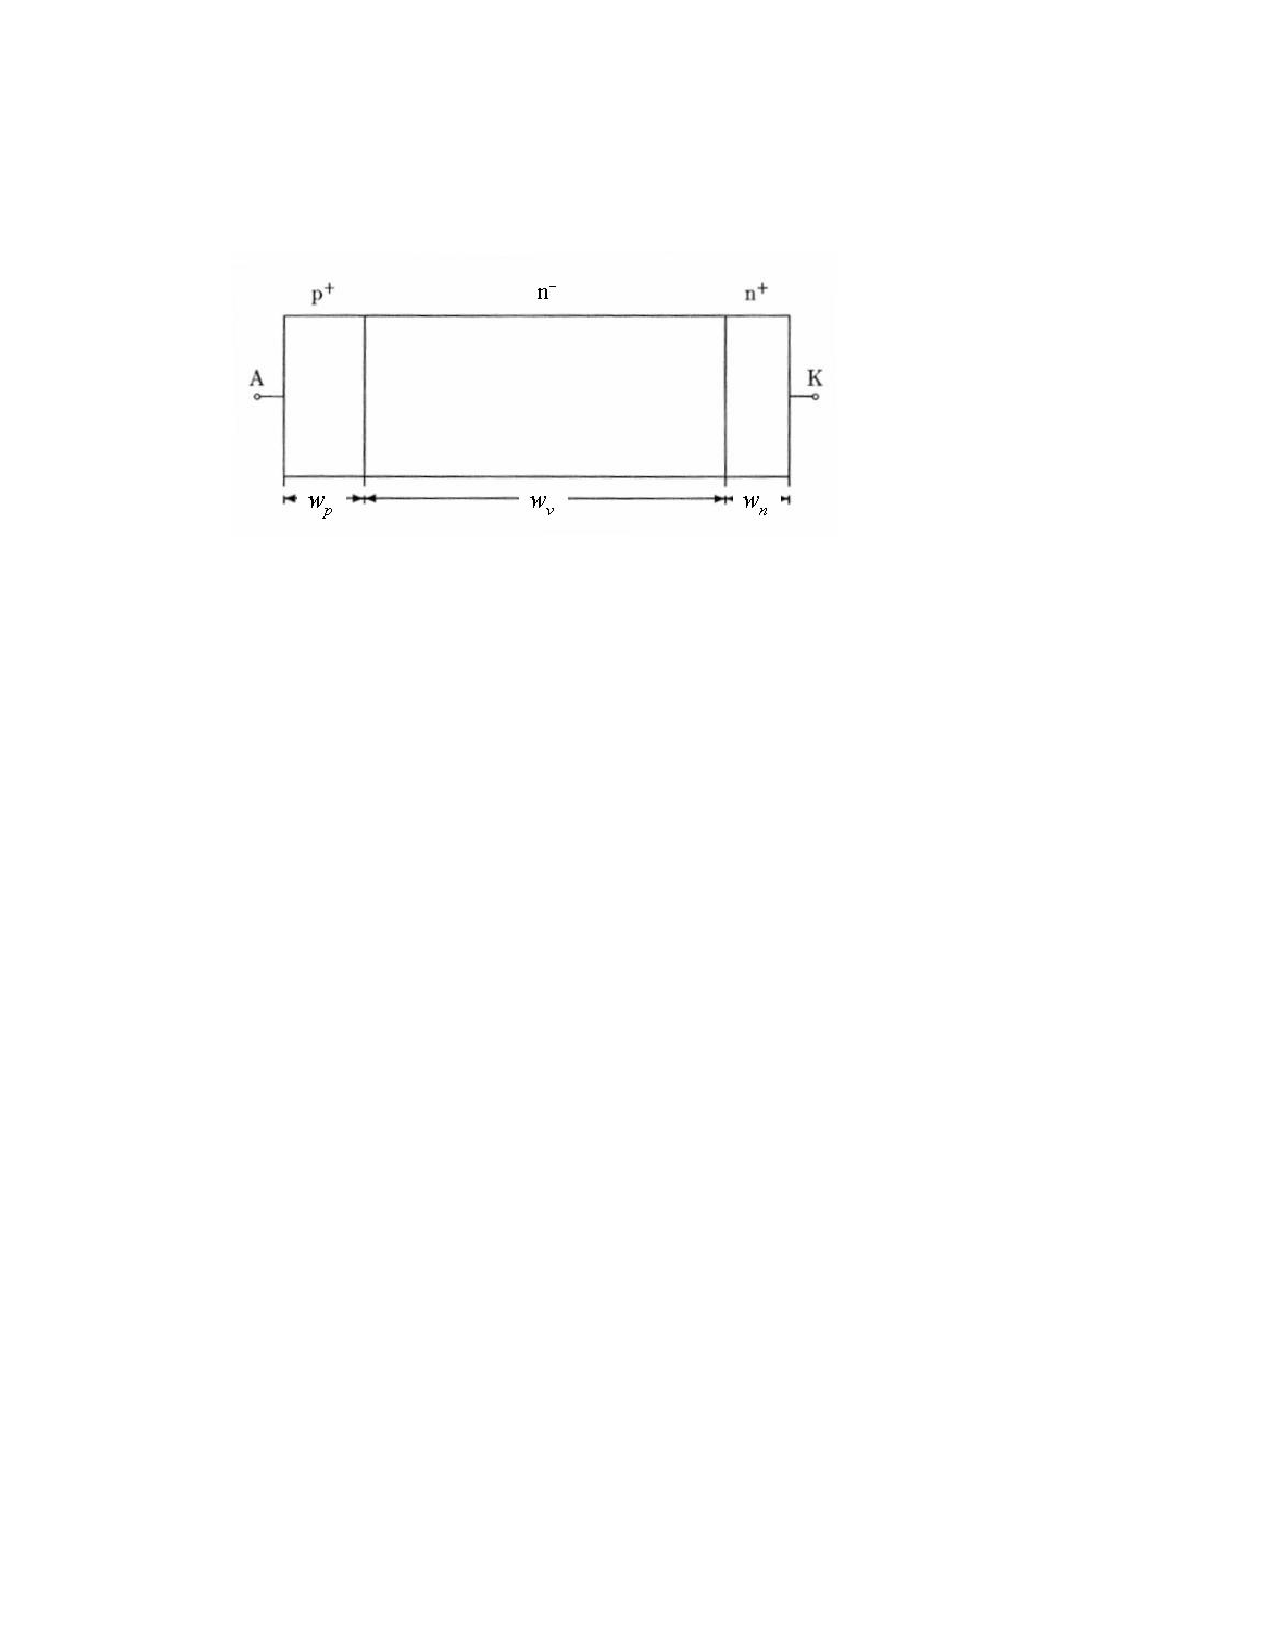
\includegraphics[width=0.8\columnwidth]{Diode_Struktur.pdf}
\end{sectionbox}
\begin{sectionbox}
\subsubsection*{Durchlasszustand}
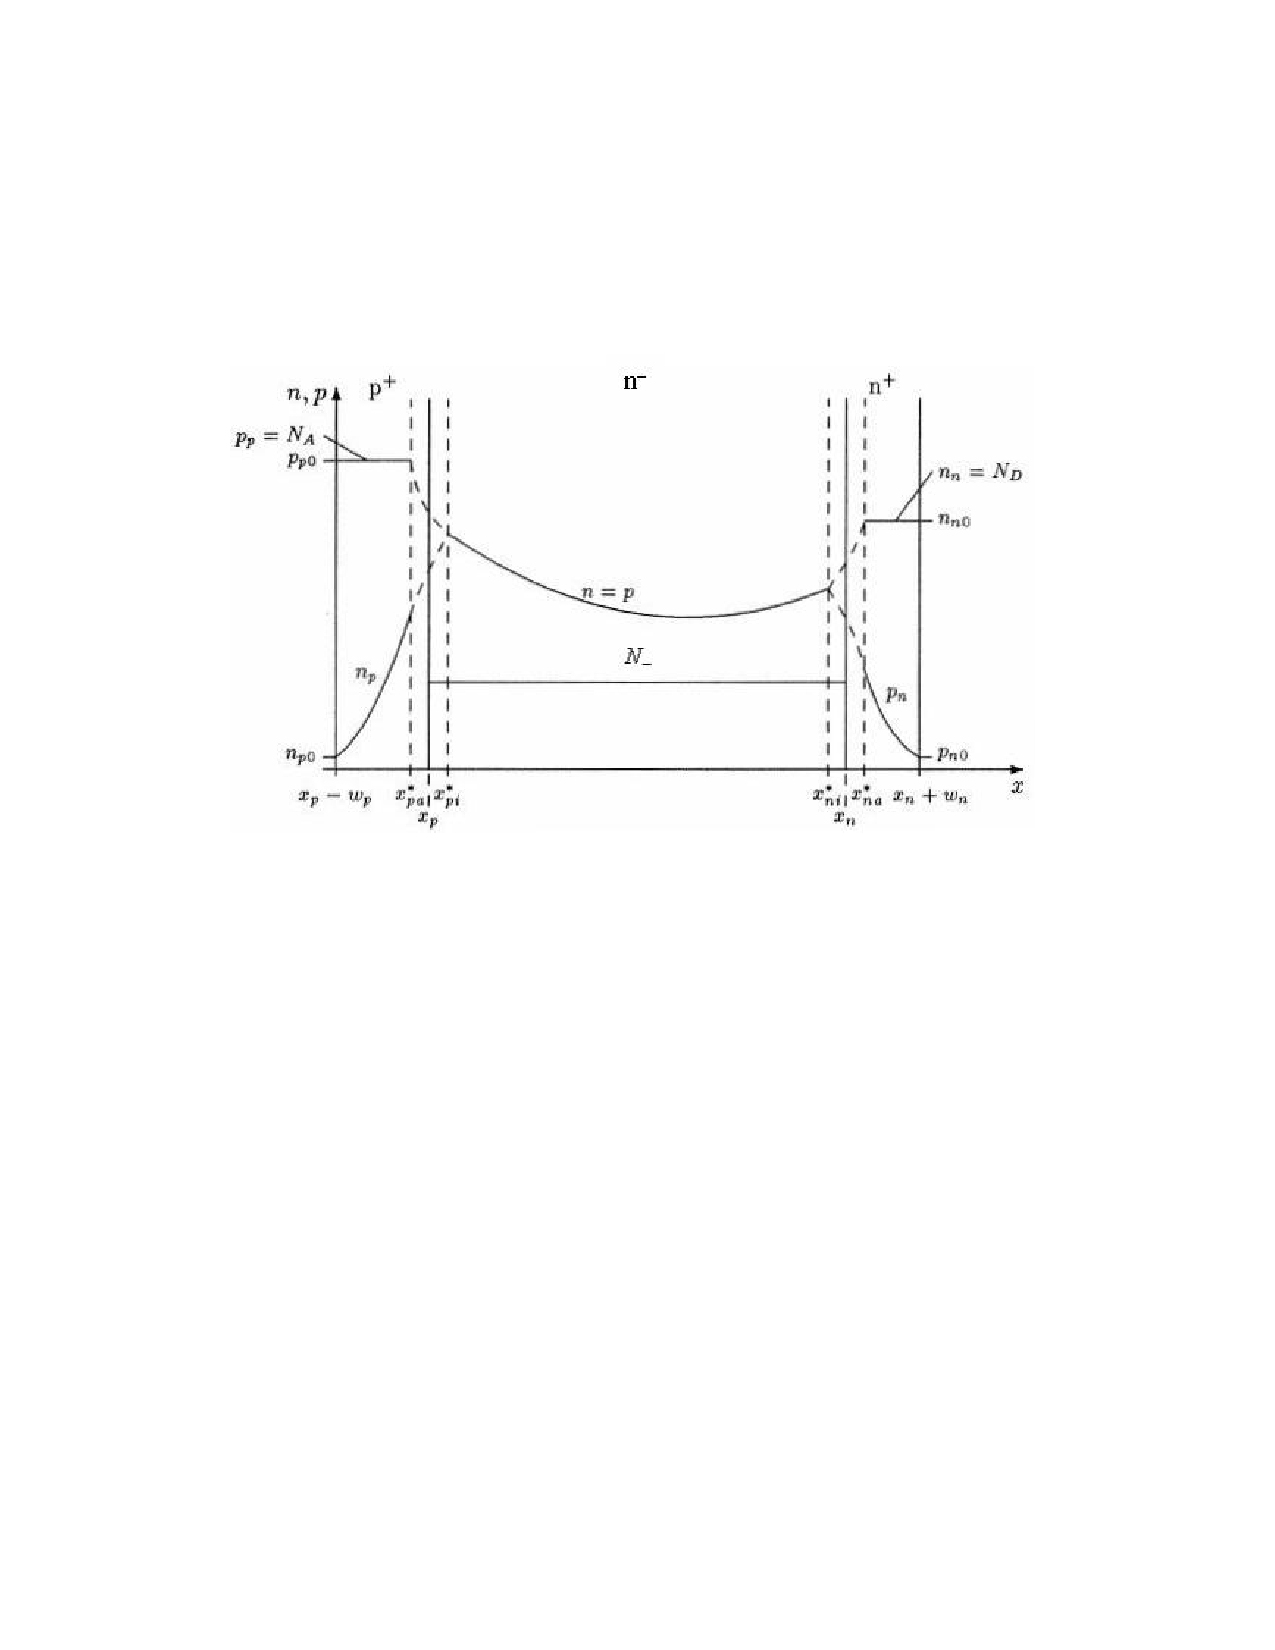
\includegraphics[width=0.8\columnwidth]{Diode_Durchlass.pdf}
\end{sectionbox}
\begin{sectionbox}

\subsubsection*{Sperrzustand}
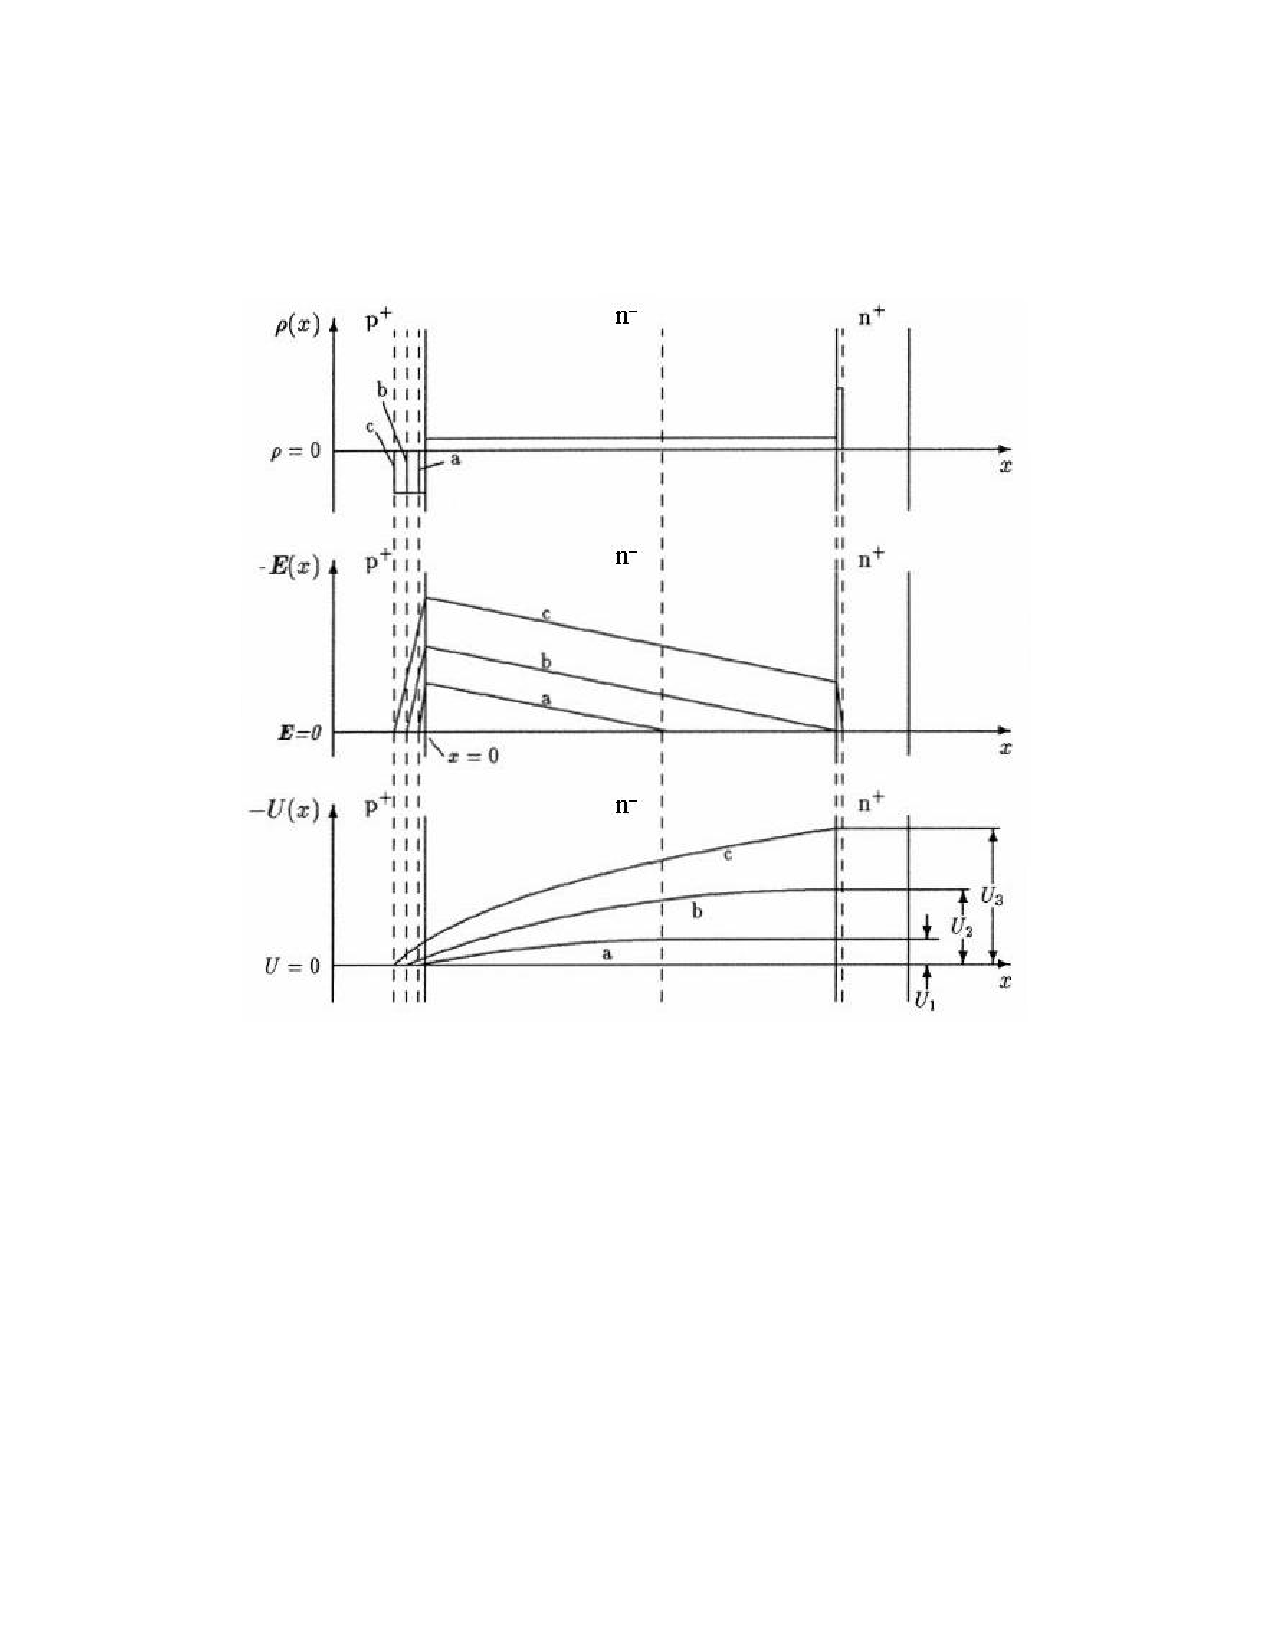
\includegraphics[width=0.8\columnwidth]{Diode_Sperr.pdf}

\end{sectionbox}
\begin{sectionbox}
\subsubsection*{Ausschaltvorgang}
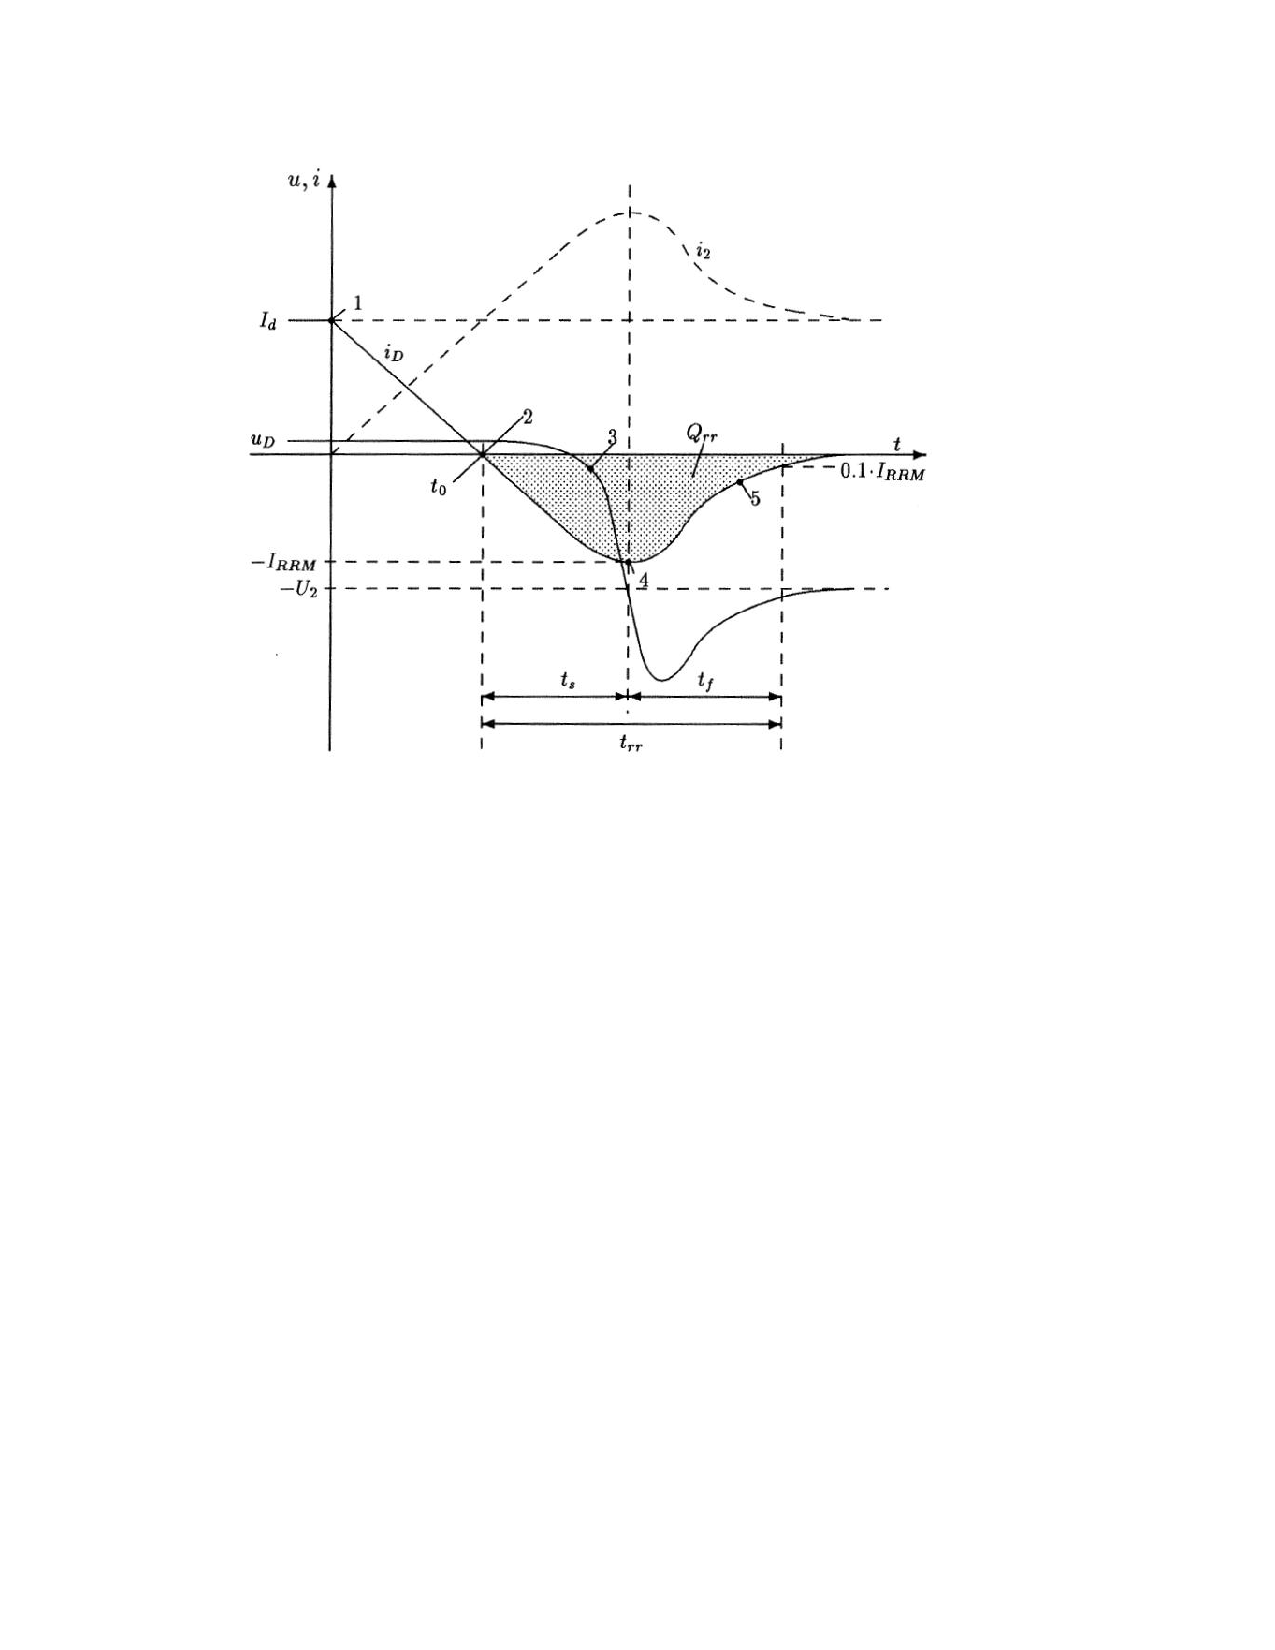
\includegraphics[width=0.8\columnwidth]{Diode_Ausschalt.pdf}

\end{sectionbox}
\begin{sectionbox}
\subsection{Thyristor}
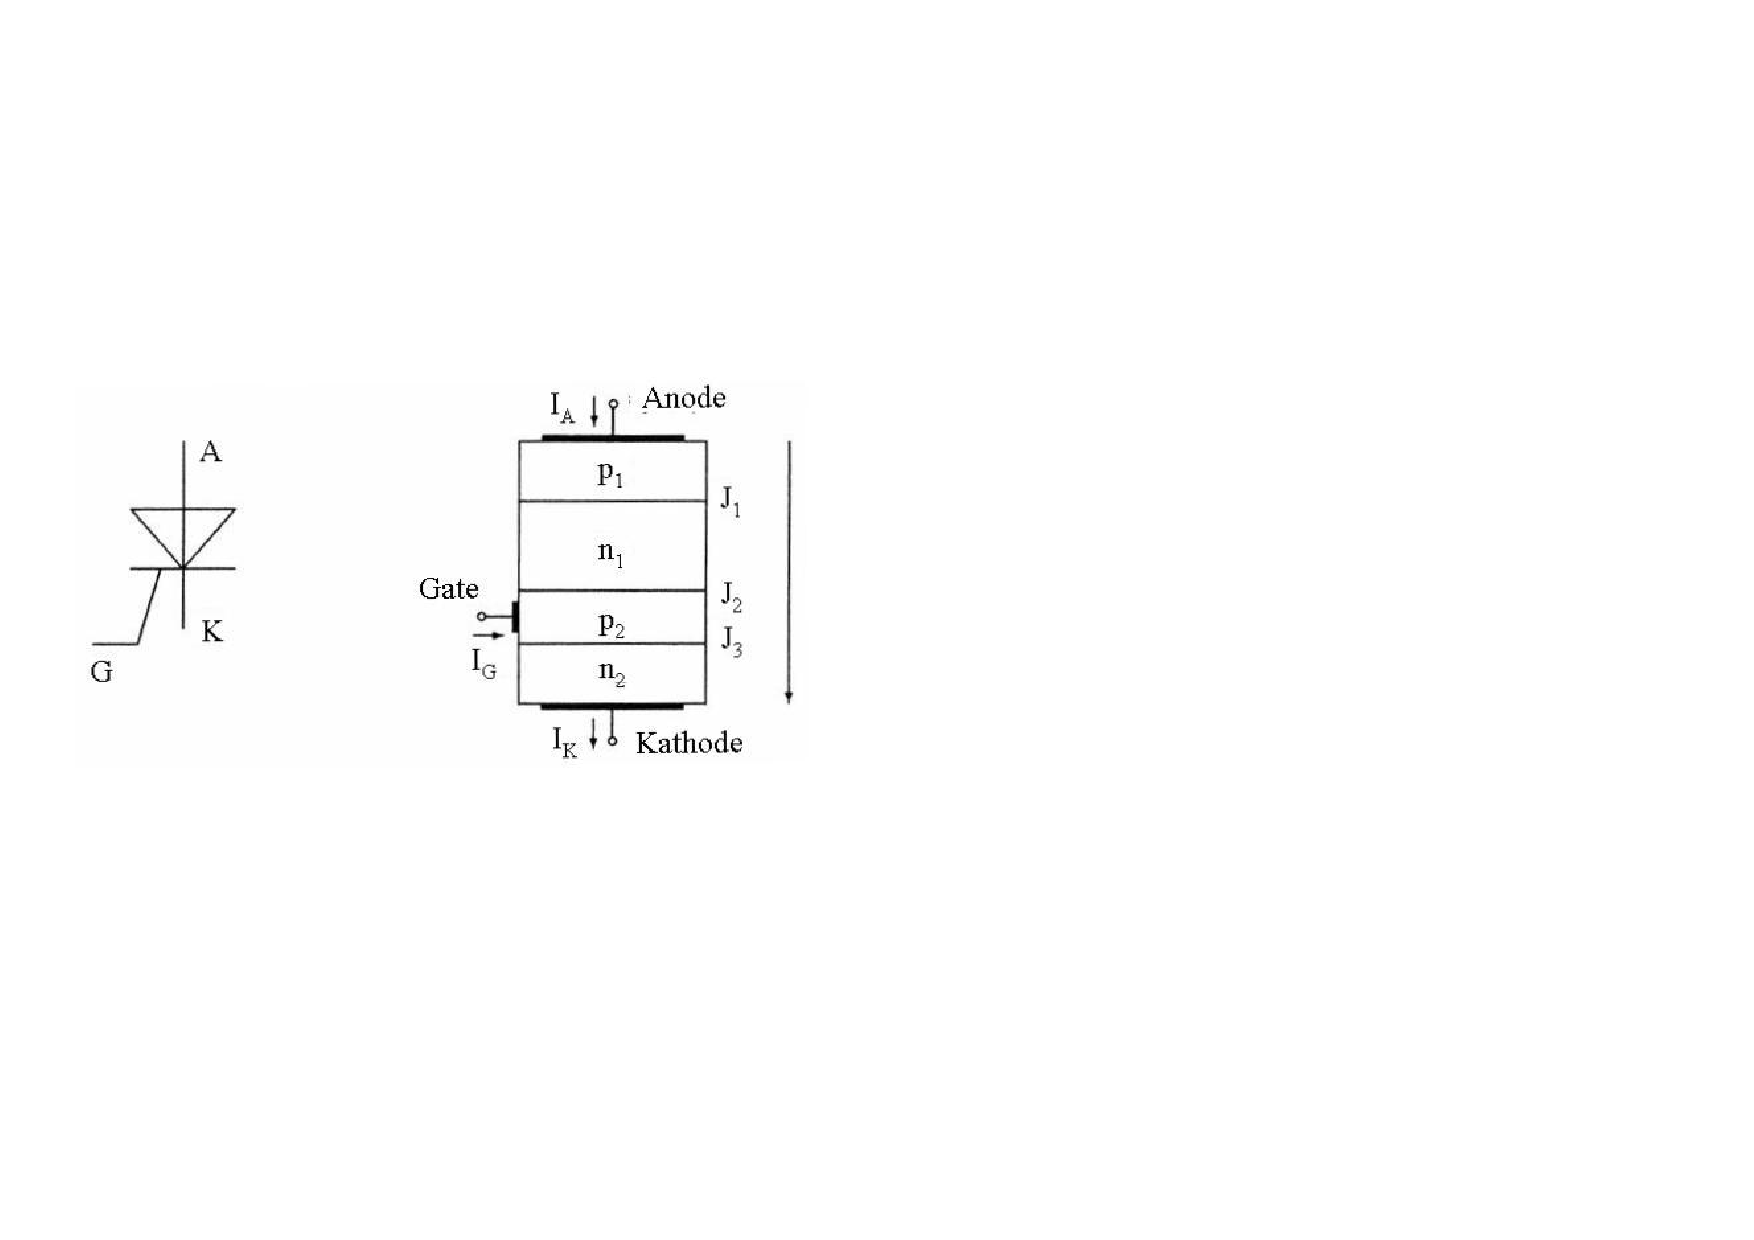
\includegraphics[width=0.8\columnwidth]{Thyristor.pdf}

\end{sectionbox}

\begin{sectionbox}
\subsection{IGCT (Integrated Gate Commutated Thyristor)}
Schaltsymbol: \\
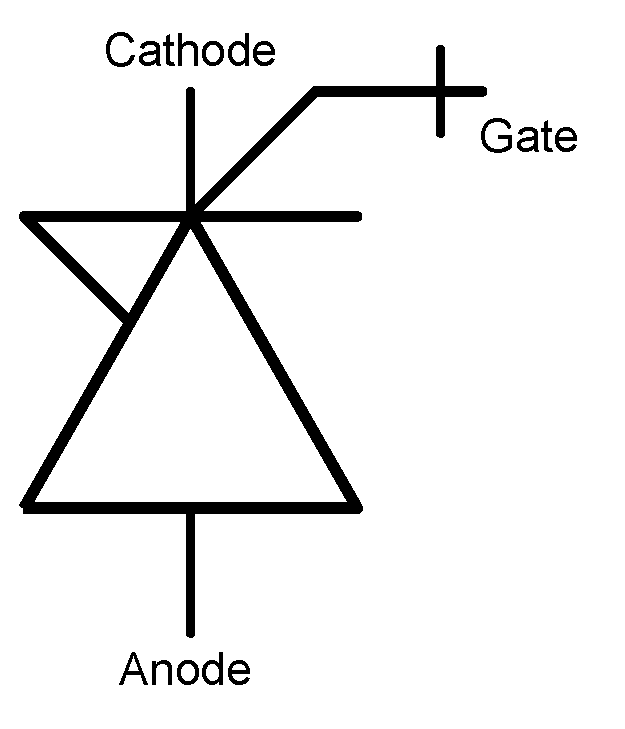
\includegraphics[width=0.2\columnwidth]{Igct_circuit_symbol5.pdf}

\end{sectionbox}

\begin{sectionbox}

\subsubsection*{Aufbau}
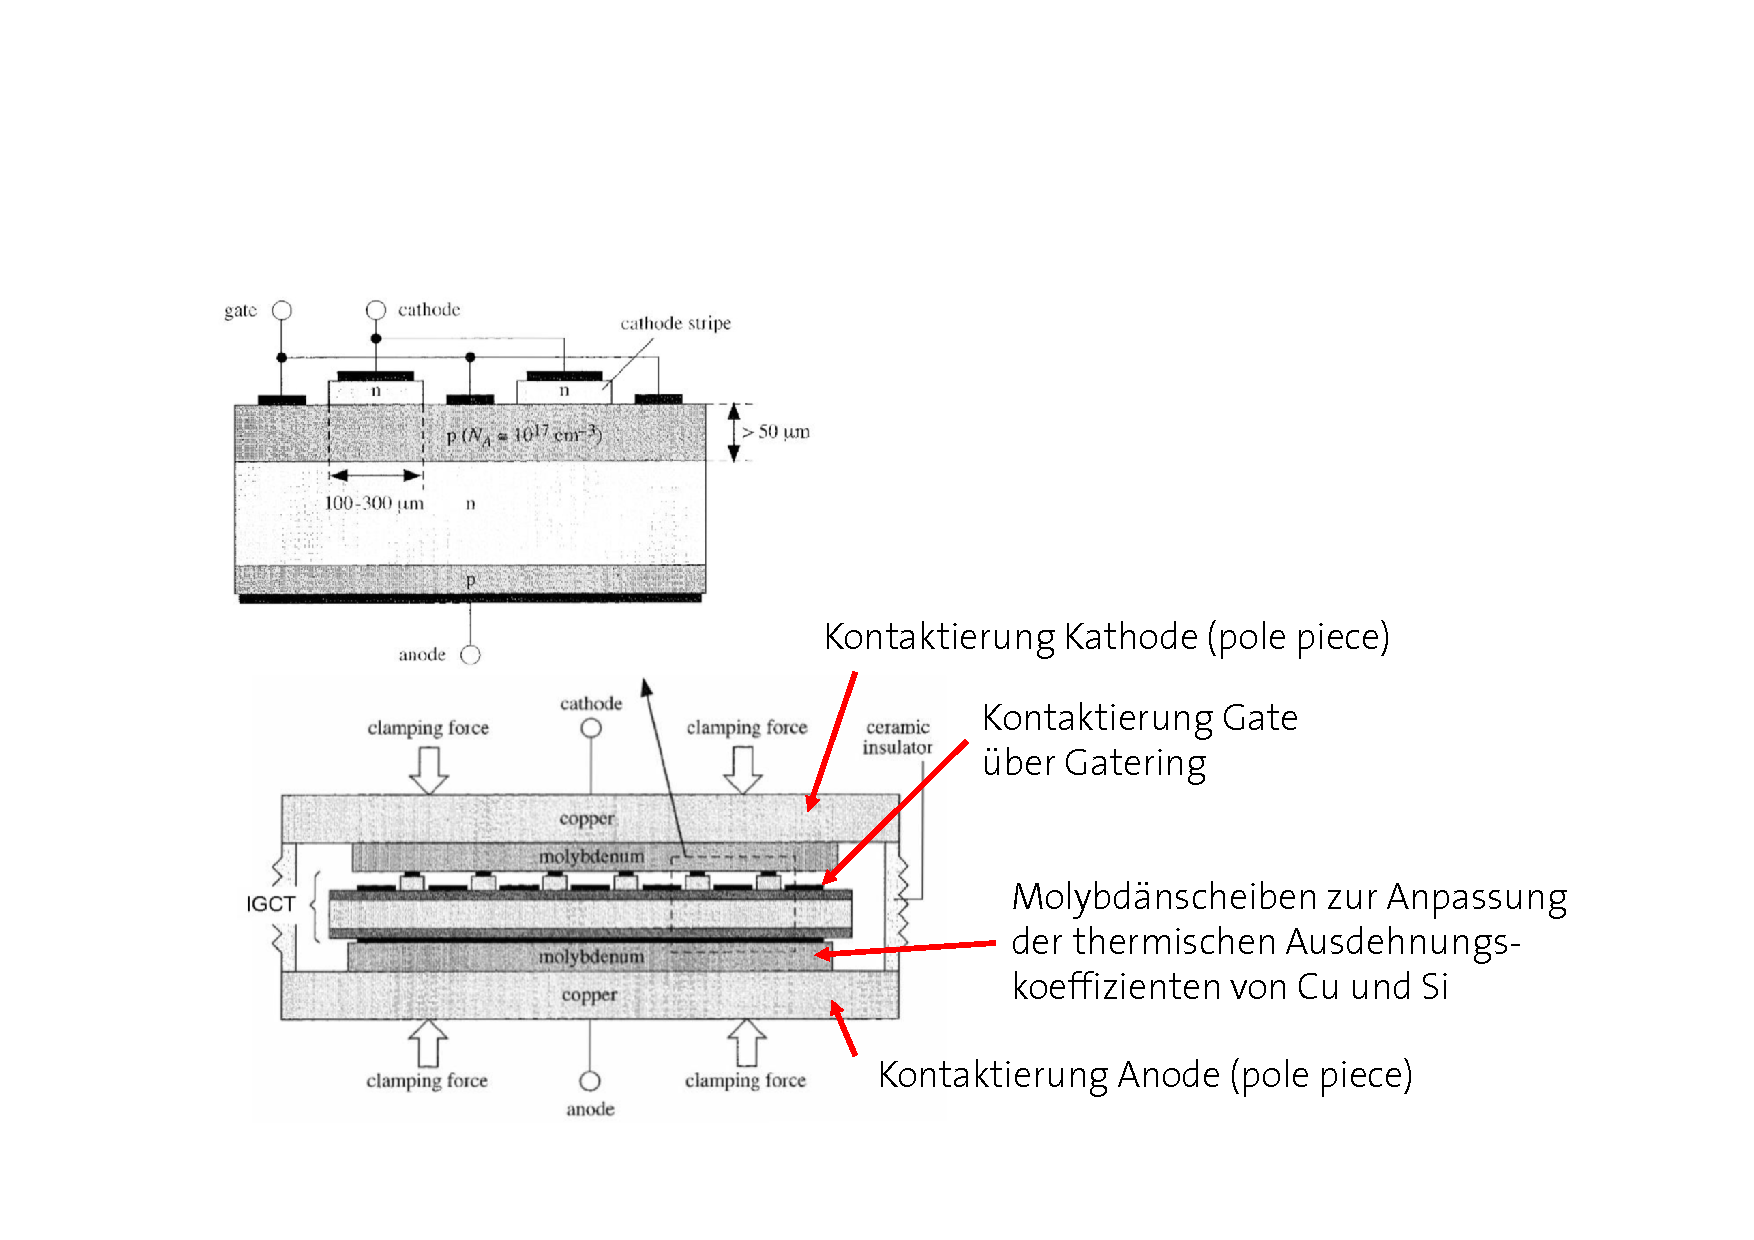
\includegraphics[width=\columnwidth]{IGCT.pdf}
\end{sectionbox}
\begin{sectionbox}
\subsubsection*{Ansteuerung}
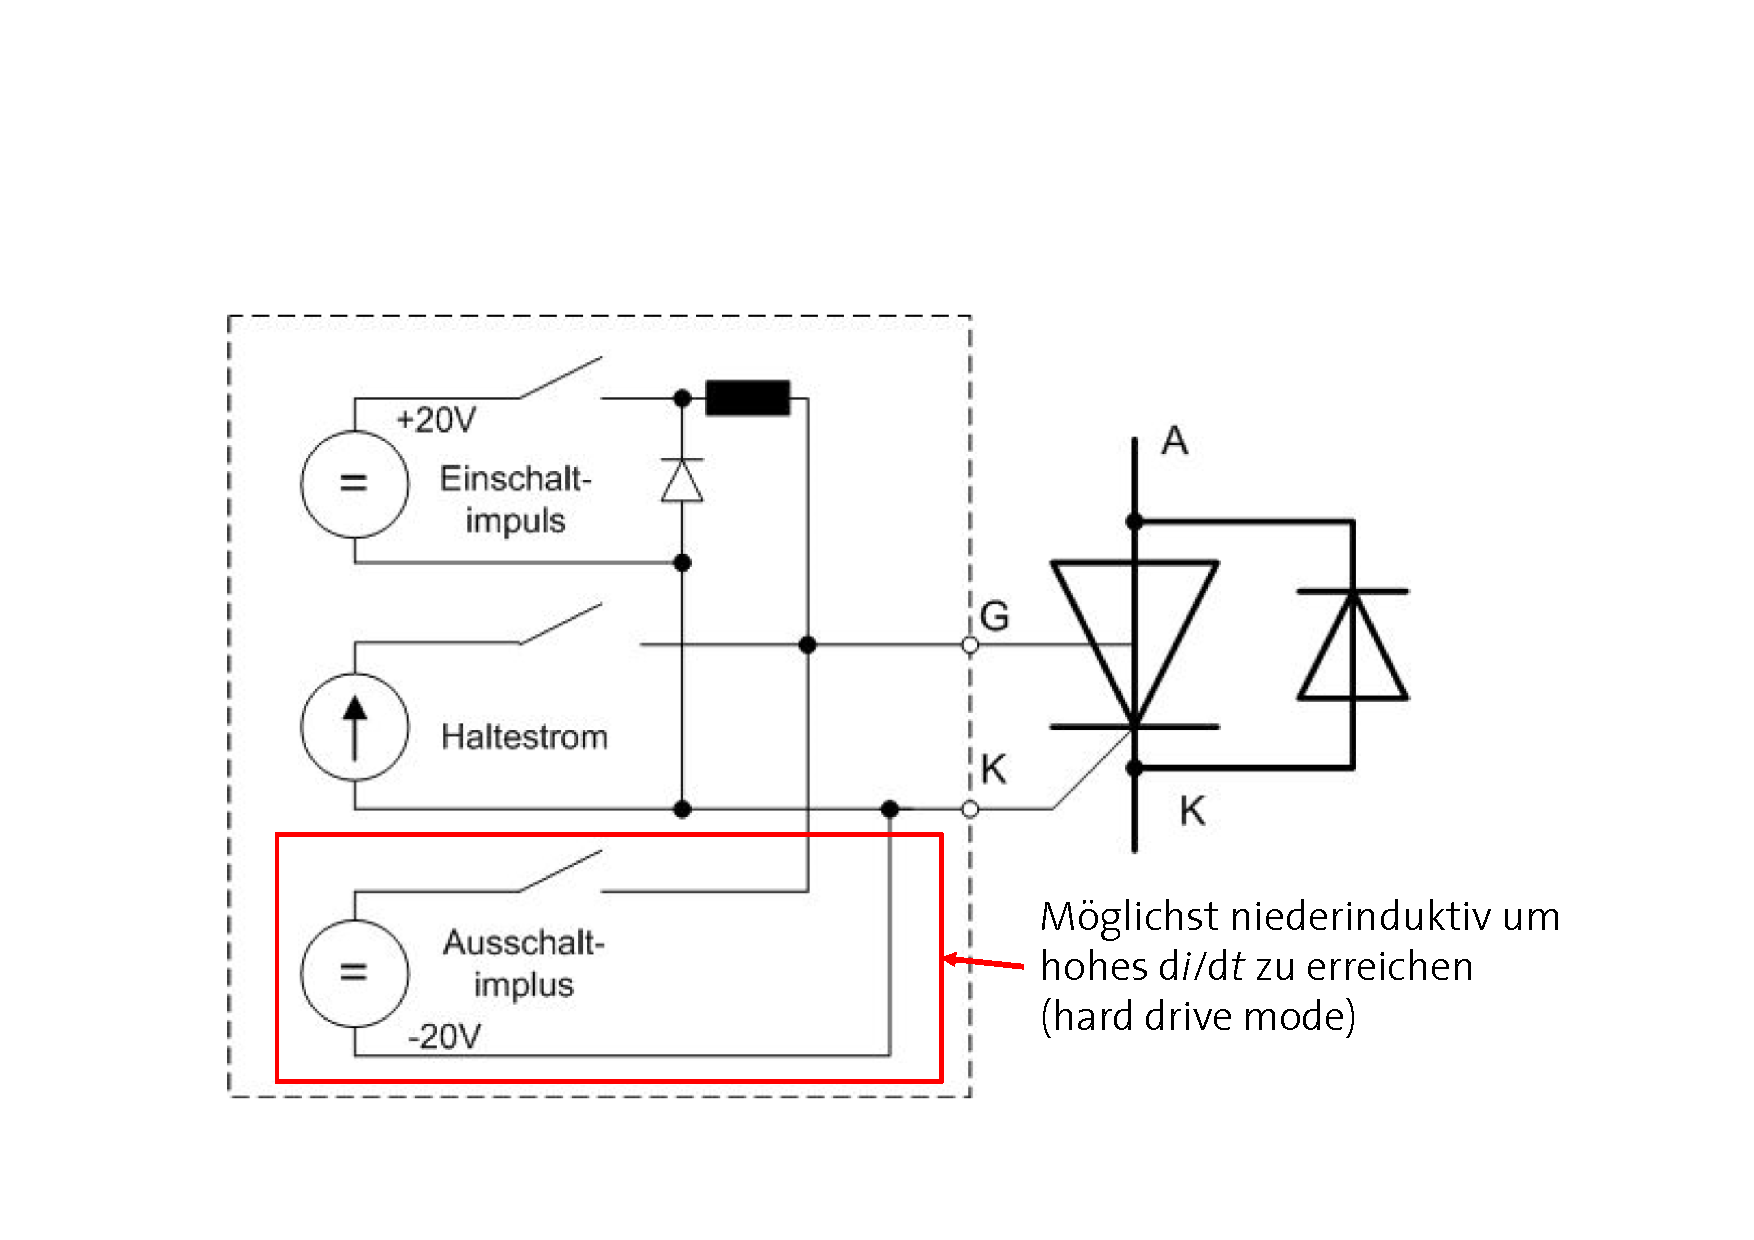
\includegraphics[width=0.7\columnwidth]{IGCT_Ansteuer.pdf}
\end{sectionbox}
\begin{sectionbox}
\subsubsection*{Ersatzmodell}
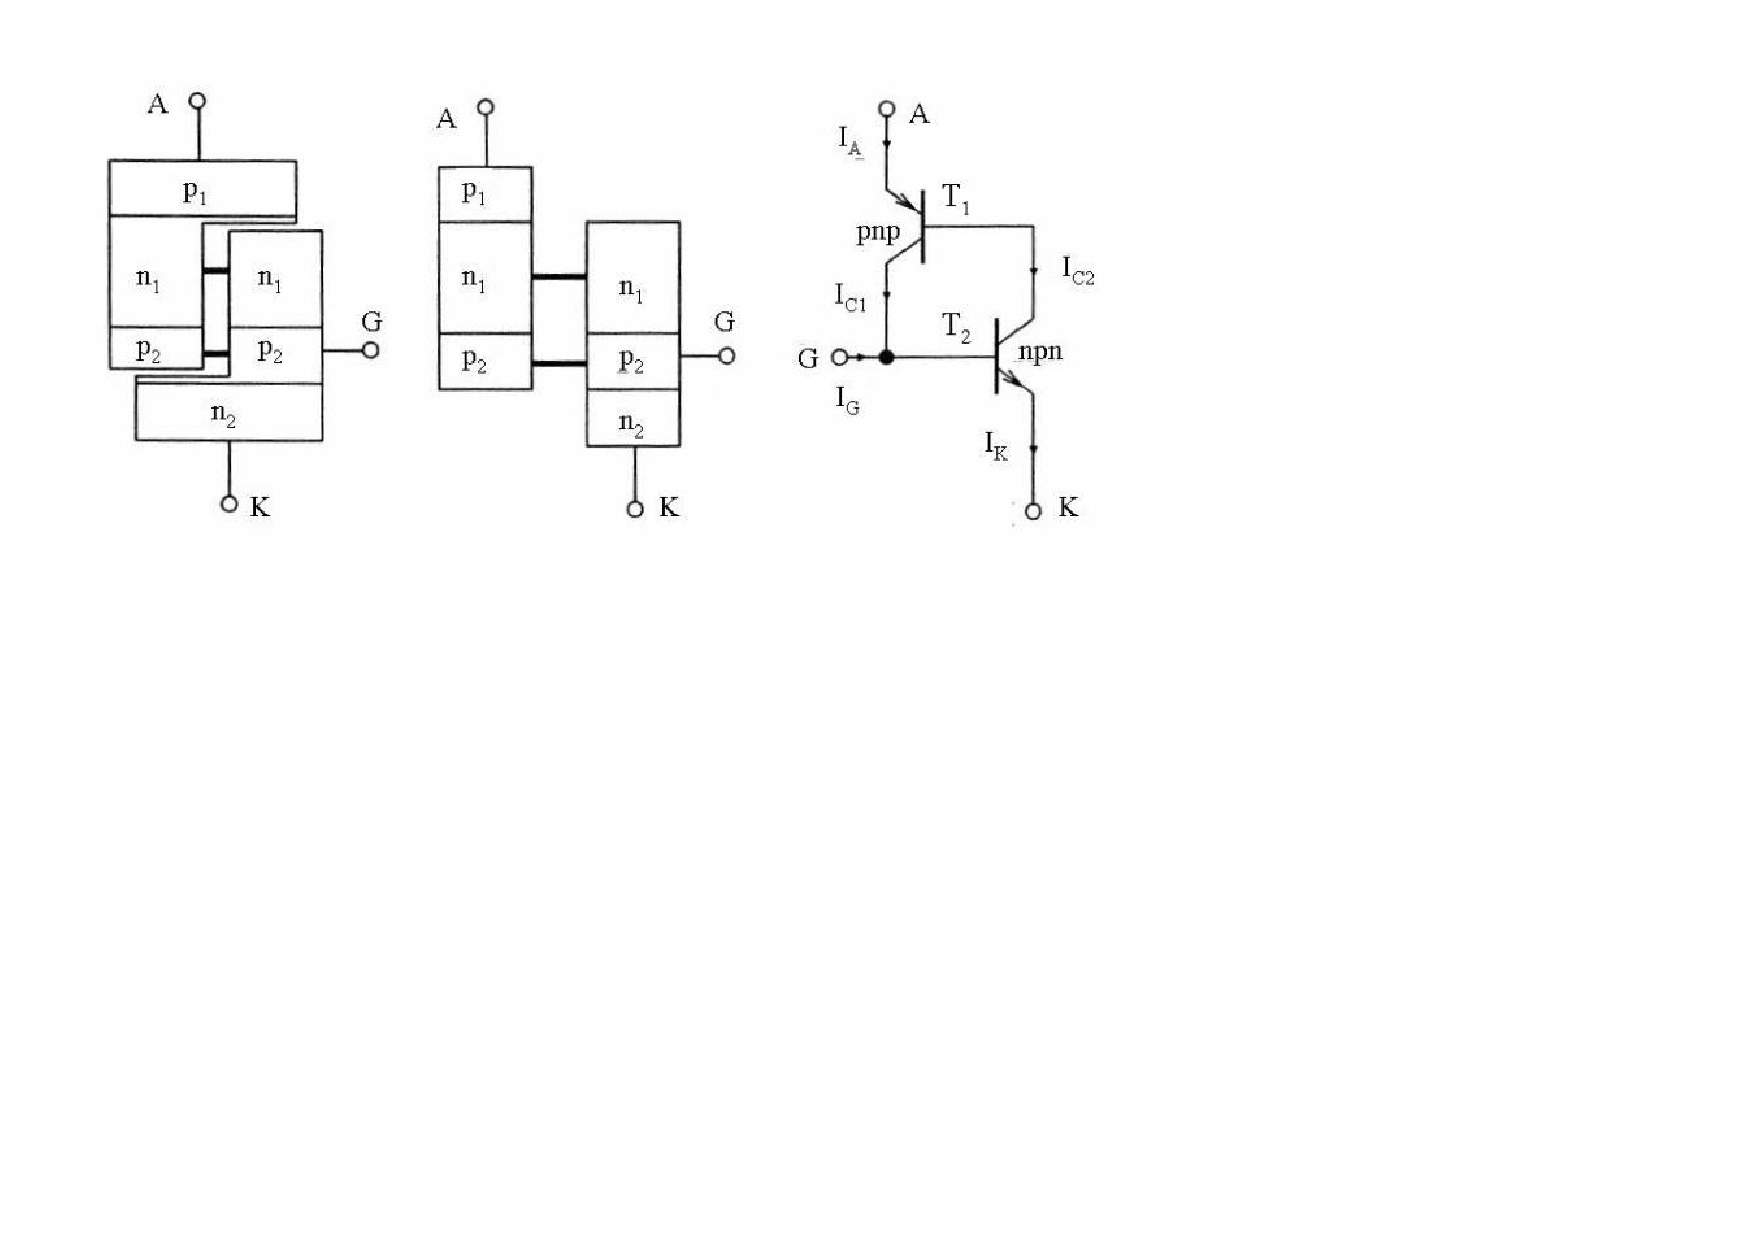
\includegraphics[width=0.7\columnwidth]{IGCT-Ersatz.pdf}

\end{sectionbox}
\begin{sectionbox}
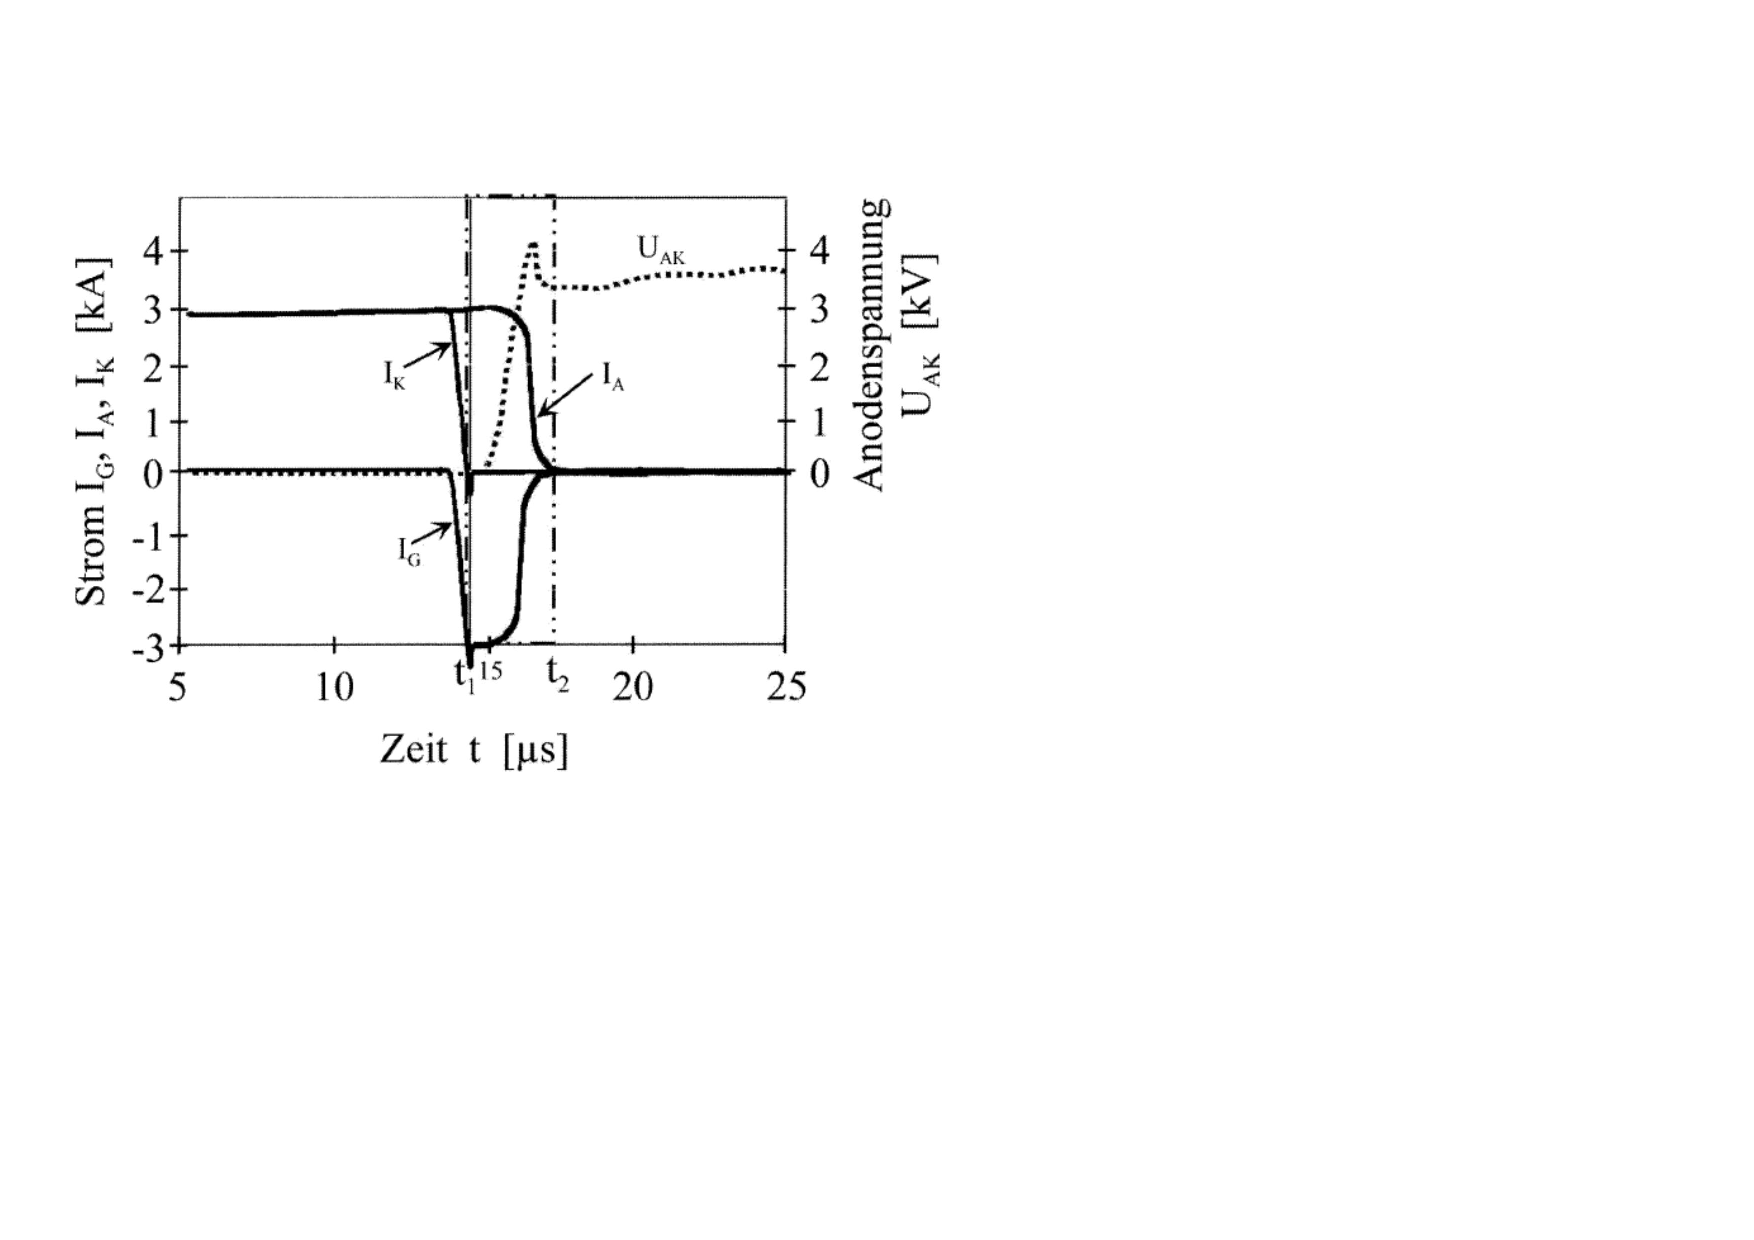
\includegraphics[width=0.7\columnwidth]{IGCT_Turnoff.pdf}

\end{sectionbox}
\begin{sectionbox}
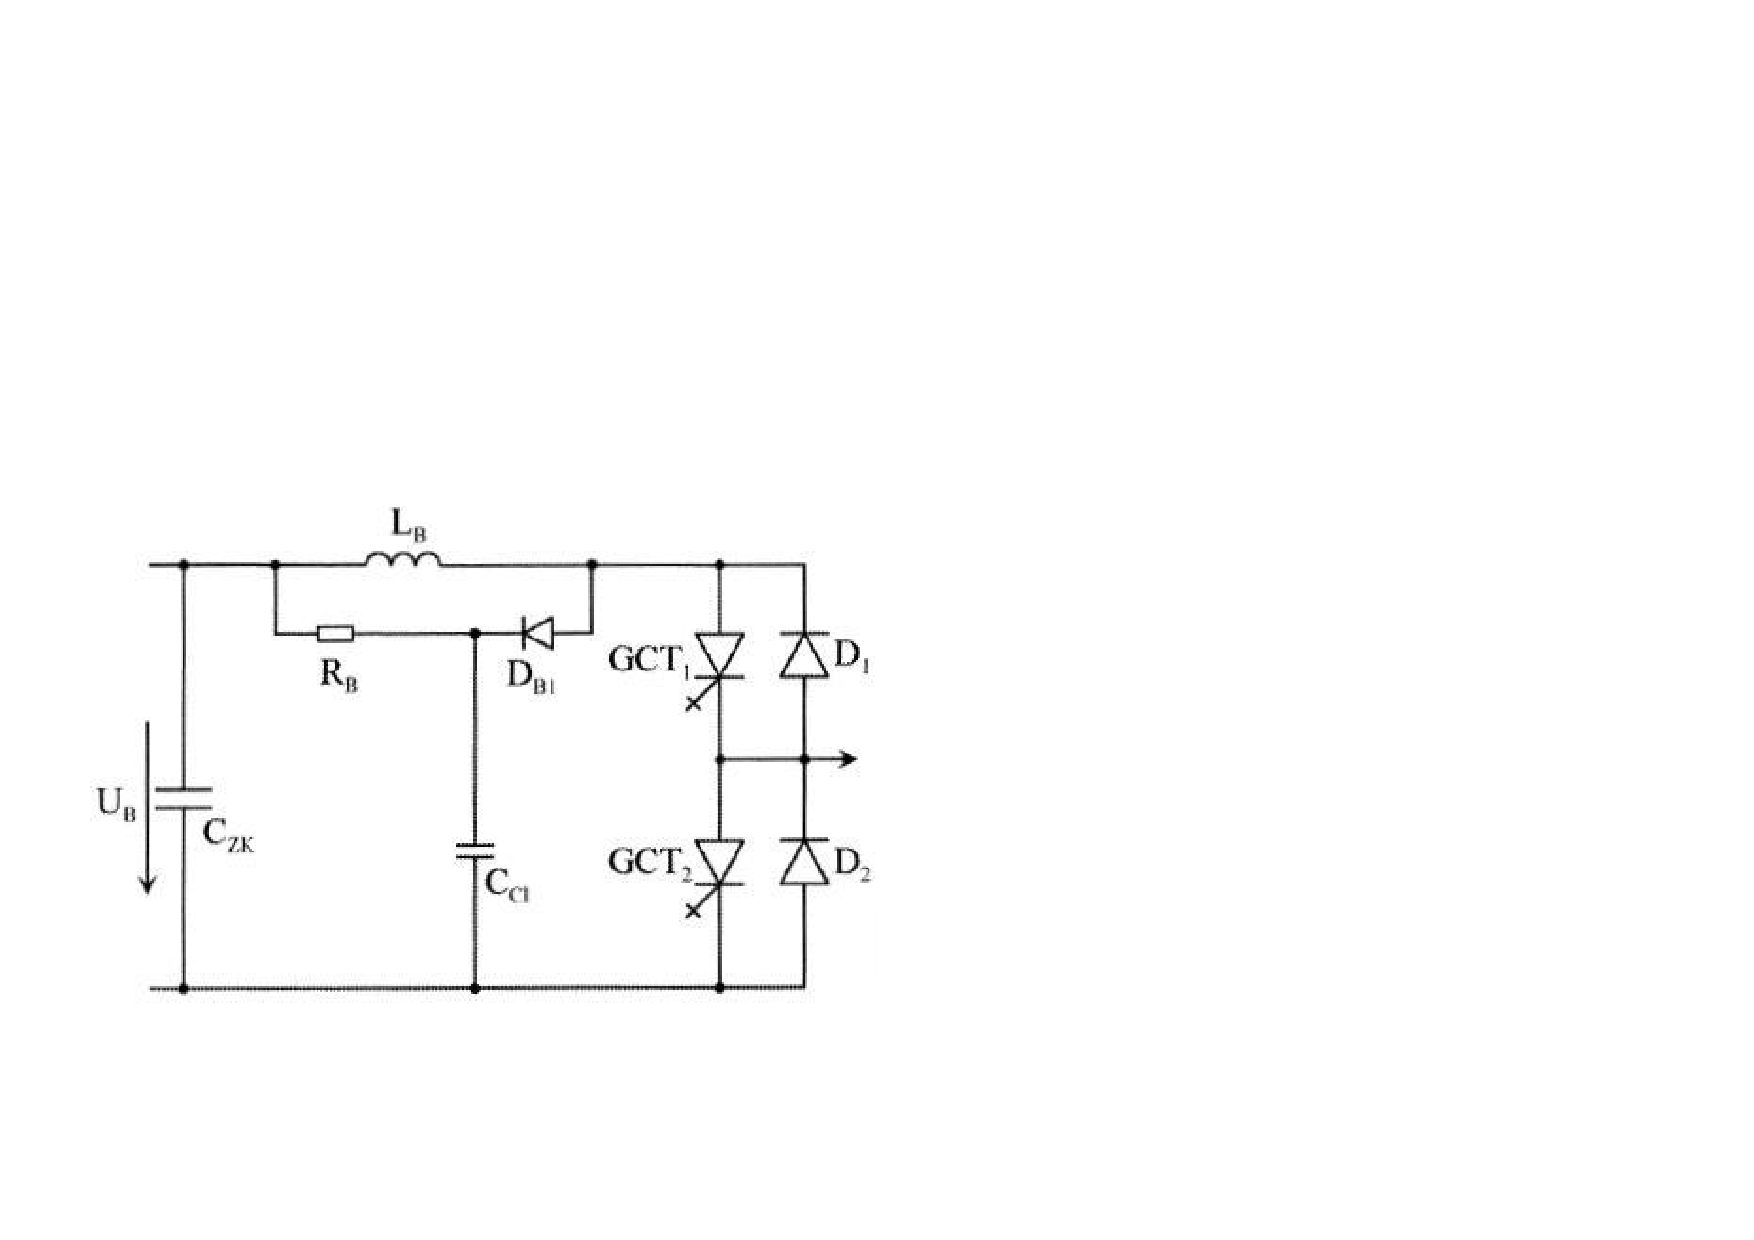
\includegraphics[width=0.7\columnwidth]{IGCT-TO-Snubber.pdf}

\end{sectionbox}



\subsection{IGBT}

\begin{sectionbox}

Schaltsymbol: \\
\ctikzset{bipoles/length=2em}
\begin{circuitikz}[scale = 0.1]
\draw   (0,0) node [nigbt, scale=1, name=igbt1] {}
(igbt1.E) node[anchor=east] {E}
(igbt1.C) node[anchor=east] {C}
(igbt1.B) node[anchor=east] {G}
    (igbt1.E) to[D, ] (igbt1.C);
\end{circuitikz}
\end{sectionbox}
\begin{sectionbox}


\subsubsection*{Aufbau}
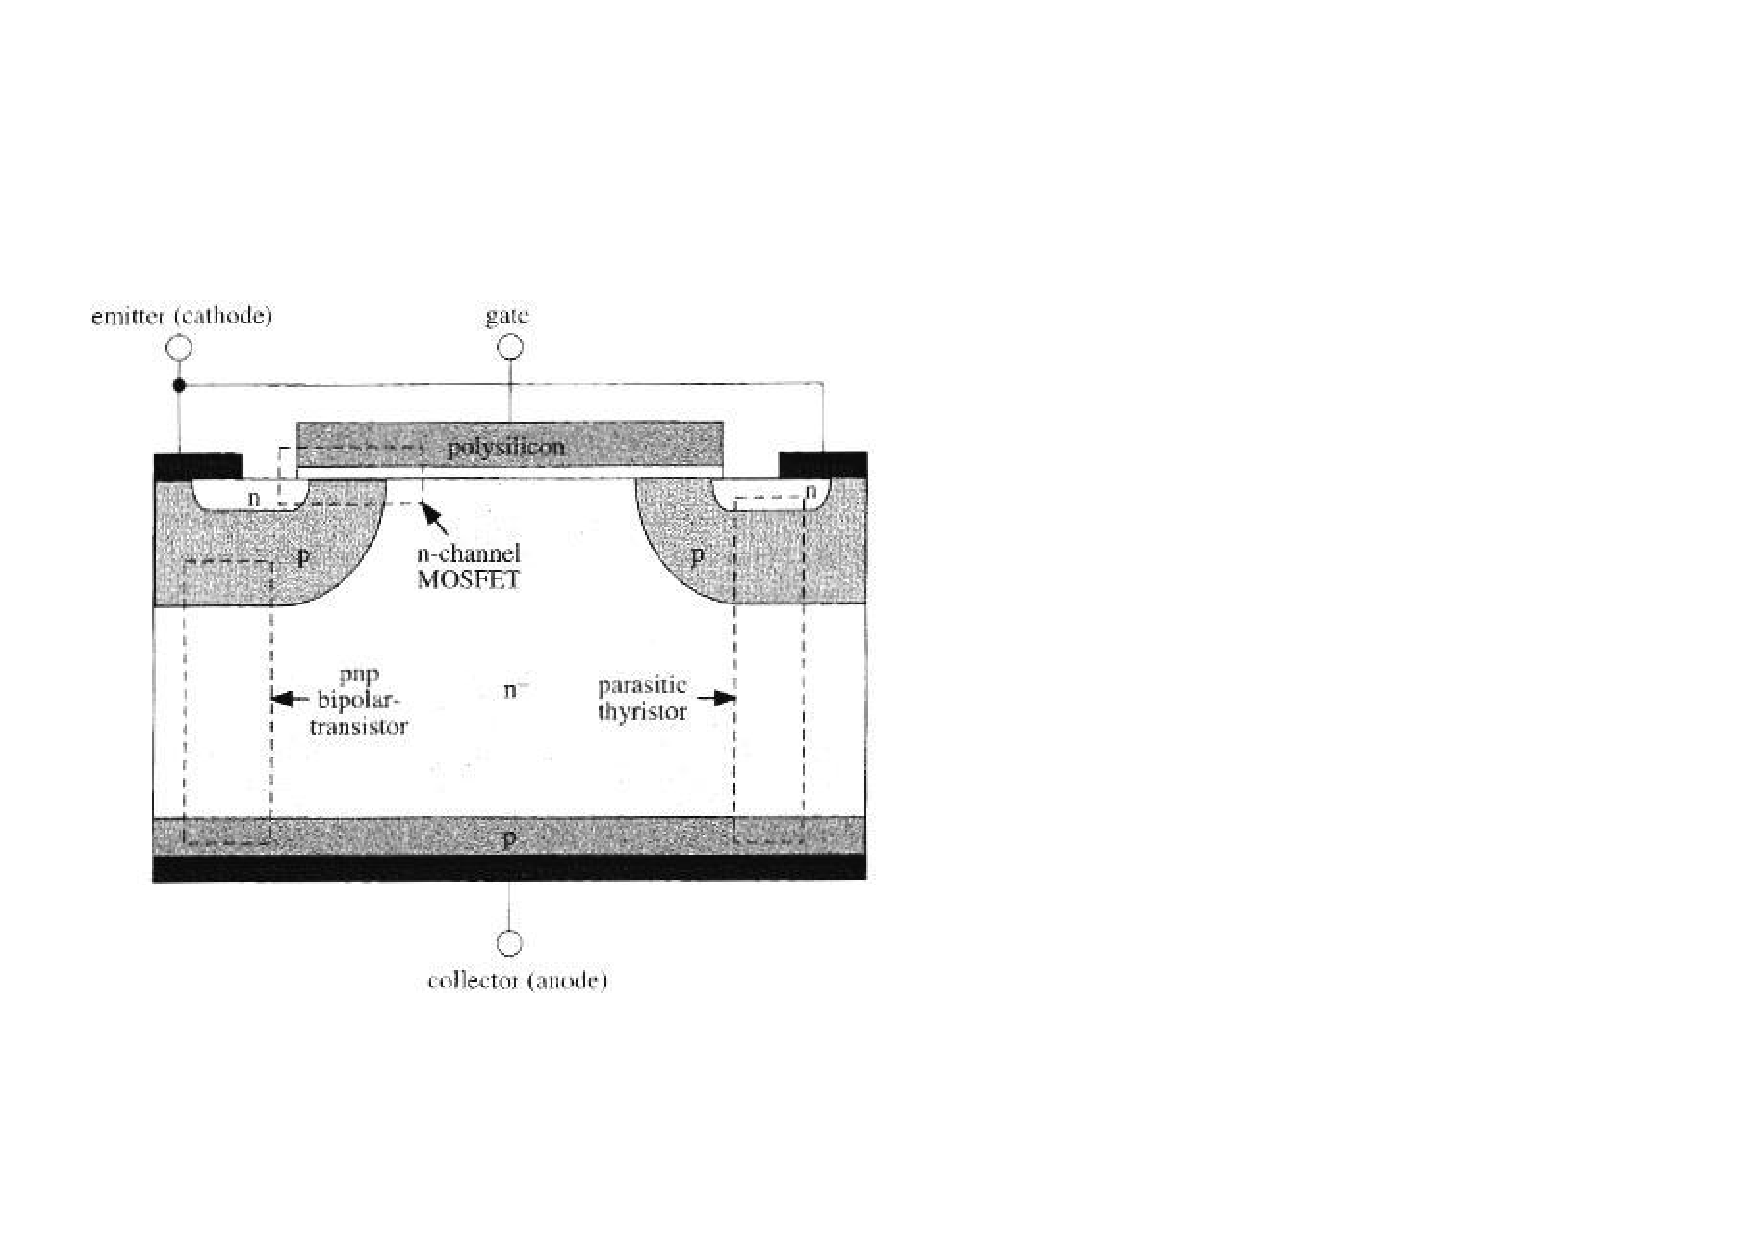
\includegraphics[width=\columnwidth]{IGBT.pdf}
\end{sectionbox}
\begin{sectionbox}
\subsubsection*{Ansteuerung}
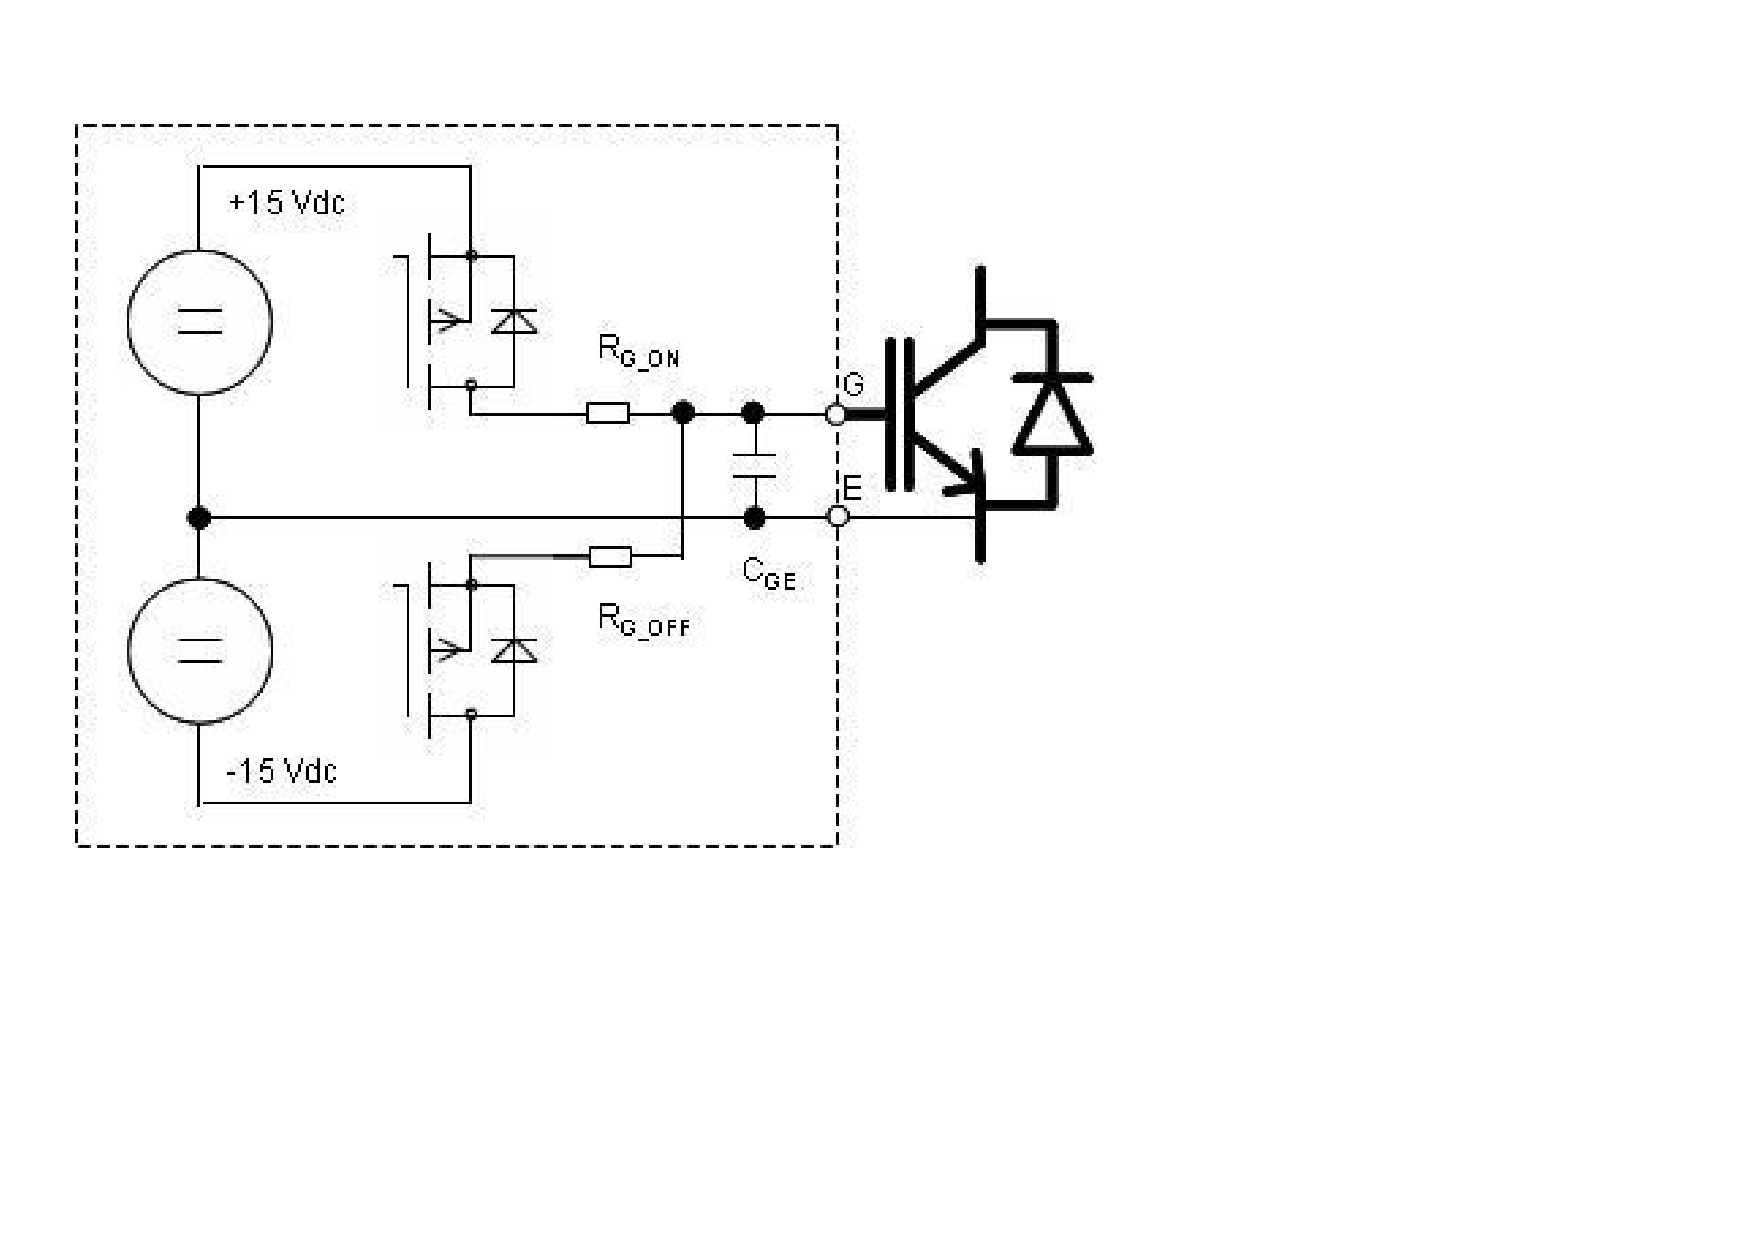
\includegraphics[width=\columnwidth]{IGBT_Ansteuer.pdf}


Zusätzlich:
\begin{itemize}
	\item Speisungsteil
	\item potentialgetrennte Ansteuerung (ggf. Optisch)
	\item Gateschutzbeschaltung (hochohmiges $R_{GE}$)
	\item $V_{CE \ir sat}$ Überwachung
	\item Soft shutdown Funktion (im Kurzschlussfall)
\end{itemize}
\end{sectionbox}

\begin{sectionbox}
\subsubsection*{Phasenbaustein eines (allgemeinen) Umrichters}
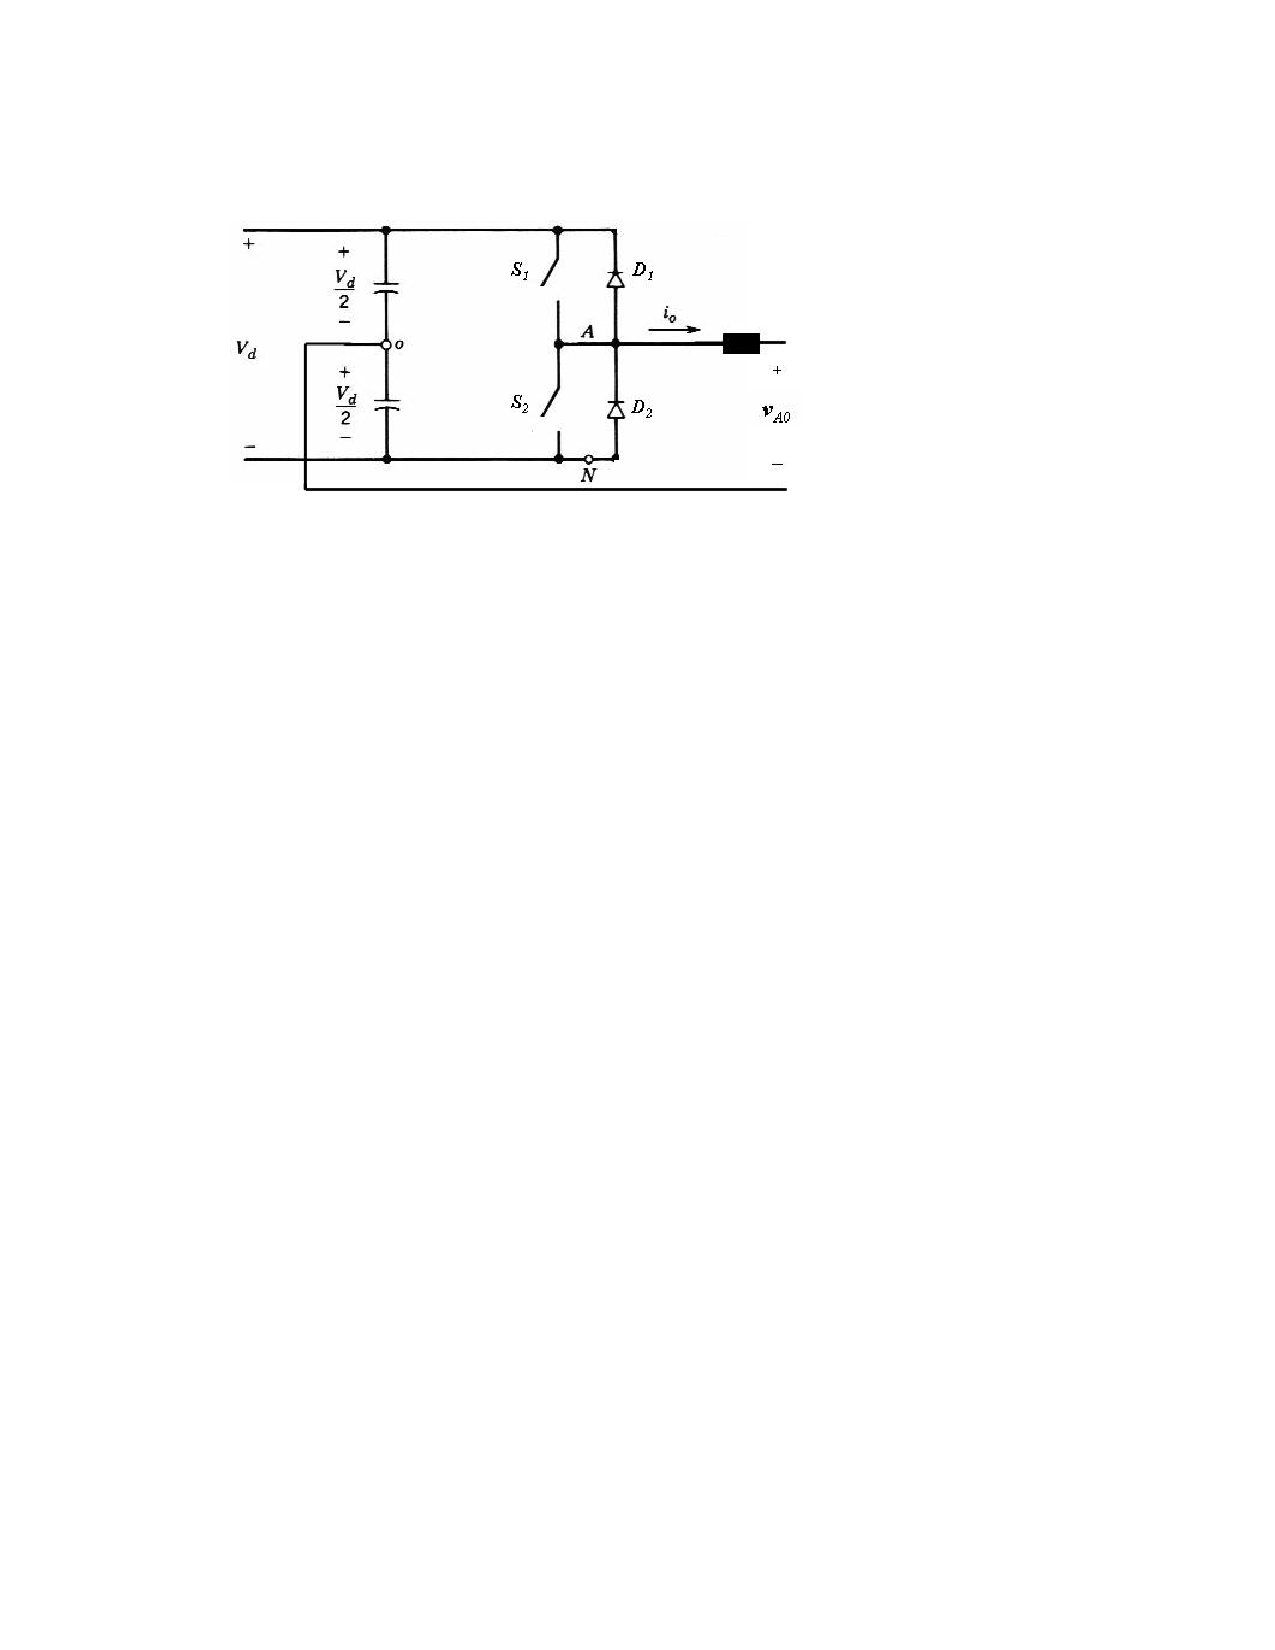
\includegraphics[width=\columnwidth]{Phasenbaustein.pdf}

\end{sectionbox}

\section{Pulswechselumrichter}
\begin{sectionbox}
\subsection{Aufbau}

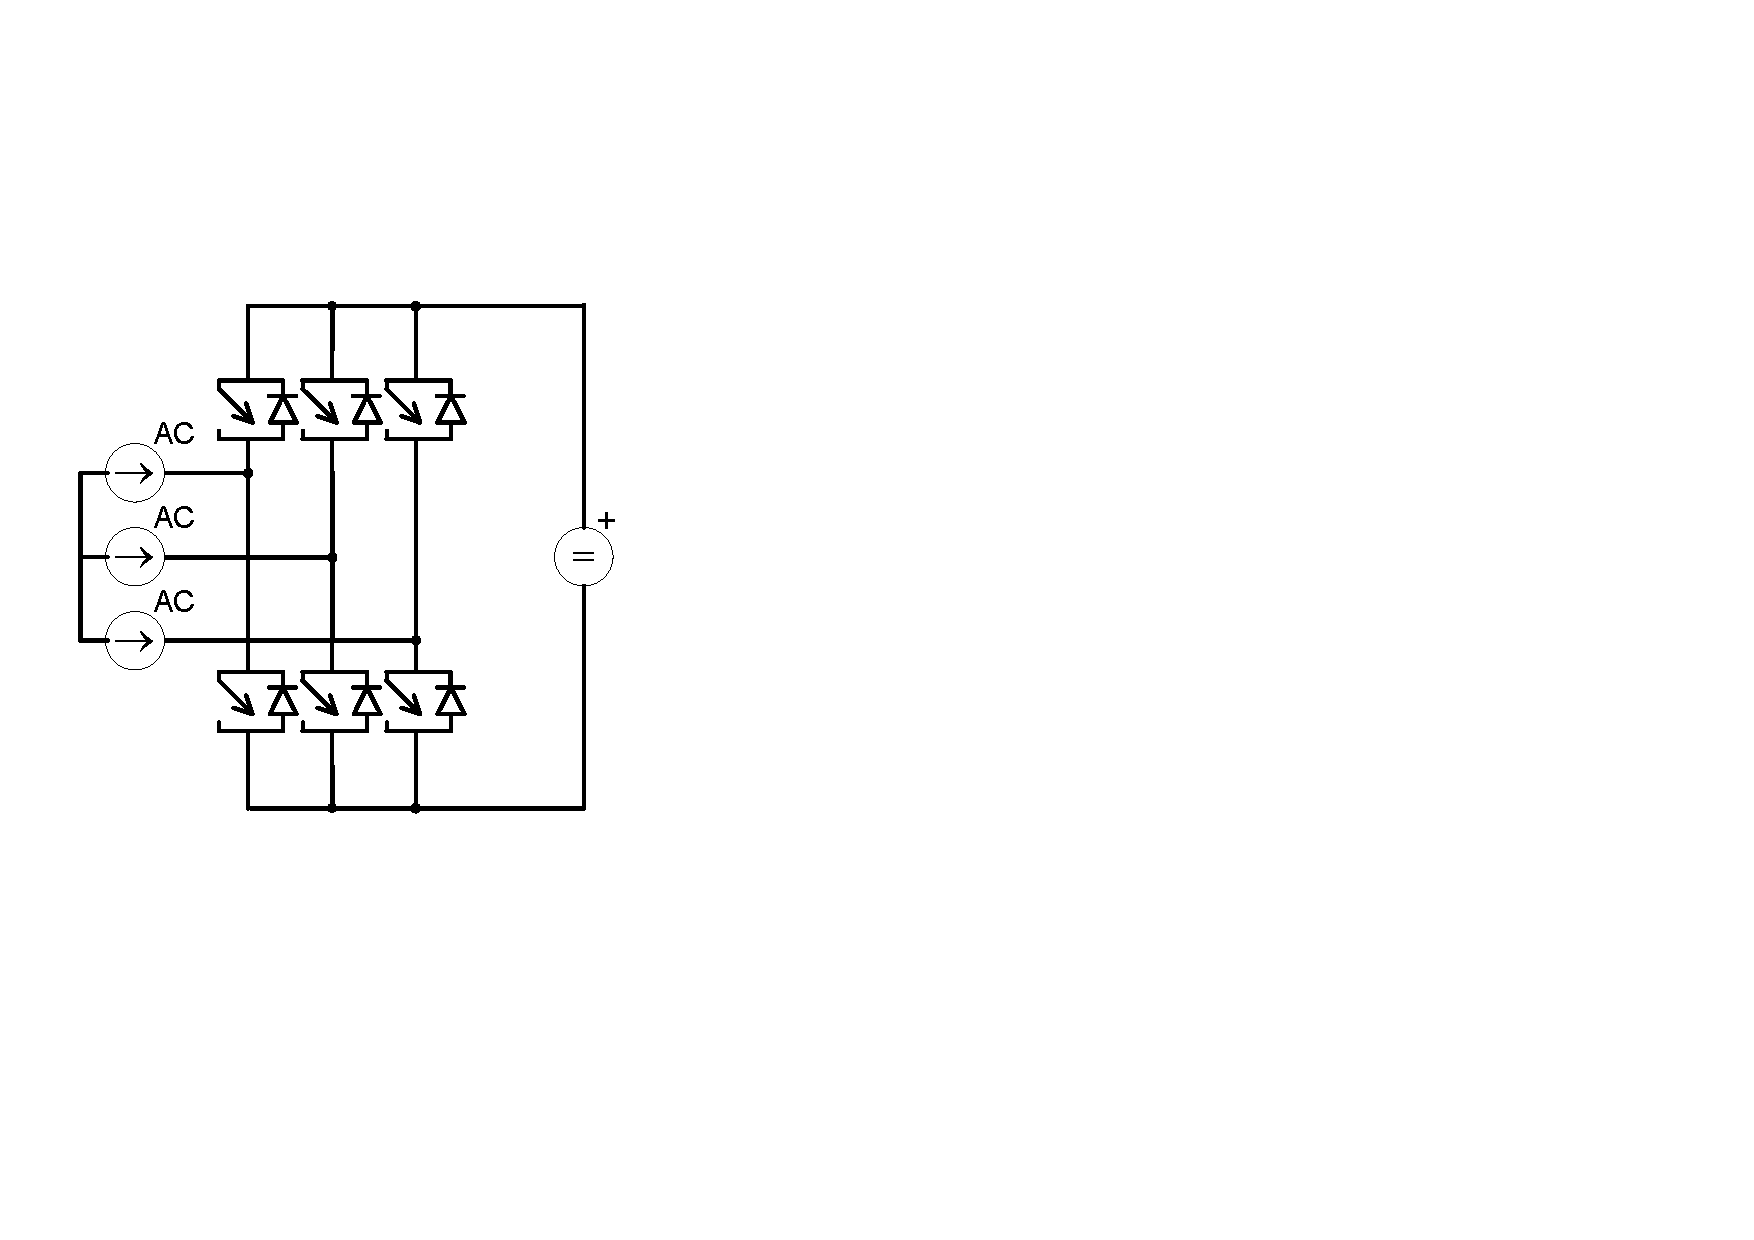
\includegraphics[width=0.6\columnwidth]{U-Umrichter.pdf}

(Amplituden-) Modulationsindex (Aussteuerung): $m_a = \frac{\hat U_{mA}}{\hat U_{CR}}$

Frequenzmodulationsverhältnis: $m_f = \frac{f_{CR}}{f_1}$
\end{sectionbox}
\begin{sectionbox}
\subsection{Grundfrequenztaktung}
Common Mode Spannung: \\
$u_{CM} (t) = u_{M0} (t) = \frac{1}{3} (u_{R0} + u_{S0} + u_{T0})$

Spitzenwert der Phasenspannung:
$\hat U_{R0_1} = \frac{2}{\pi} U_d$


Amplitude der Grundwelle der verketteten Ausgangsspannung: \\
$U_{LL_1} = \frac{\sqrt 6}{\pi} U_d$

Oberschwingungen der Ausgangsspannung: \\
$U_{LL_v} = \frac{\sqrt 6}{\pi} \frac{U_d}{v}$ für $v = 6n \pm 1 (n = 1, 2, 3, \ldots)$
\end{sectionbox}
\begin{sectionbox}
\subsection{PWM}  
\end{sectionbox}

\section{U/f Steuerung}

\begin{sectionbox}

\subsection{Steuerung ohne Drehzahlgeber}
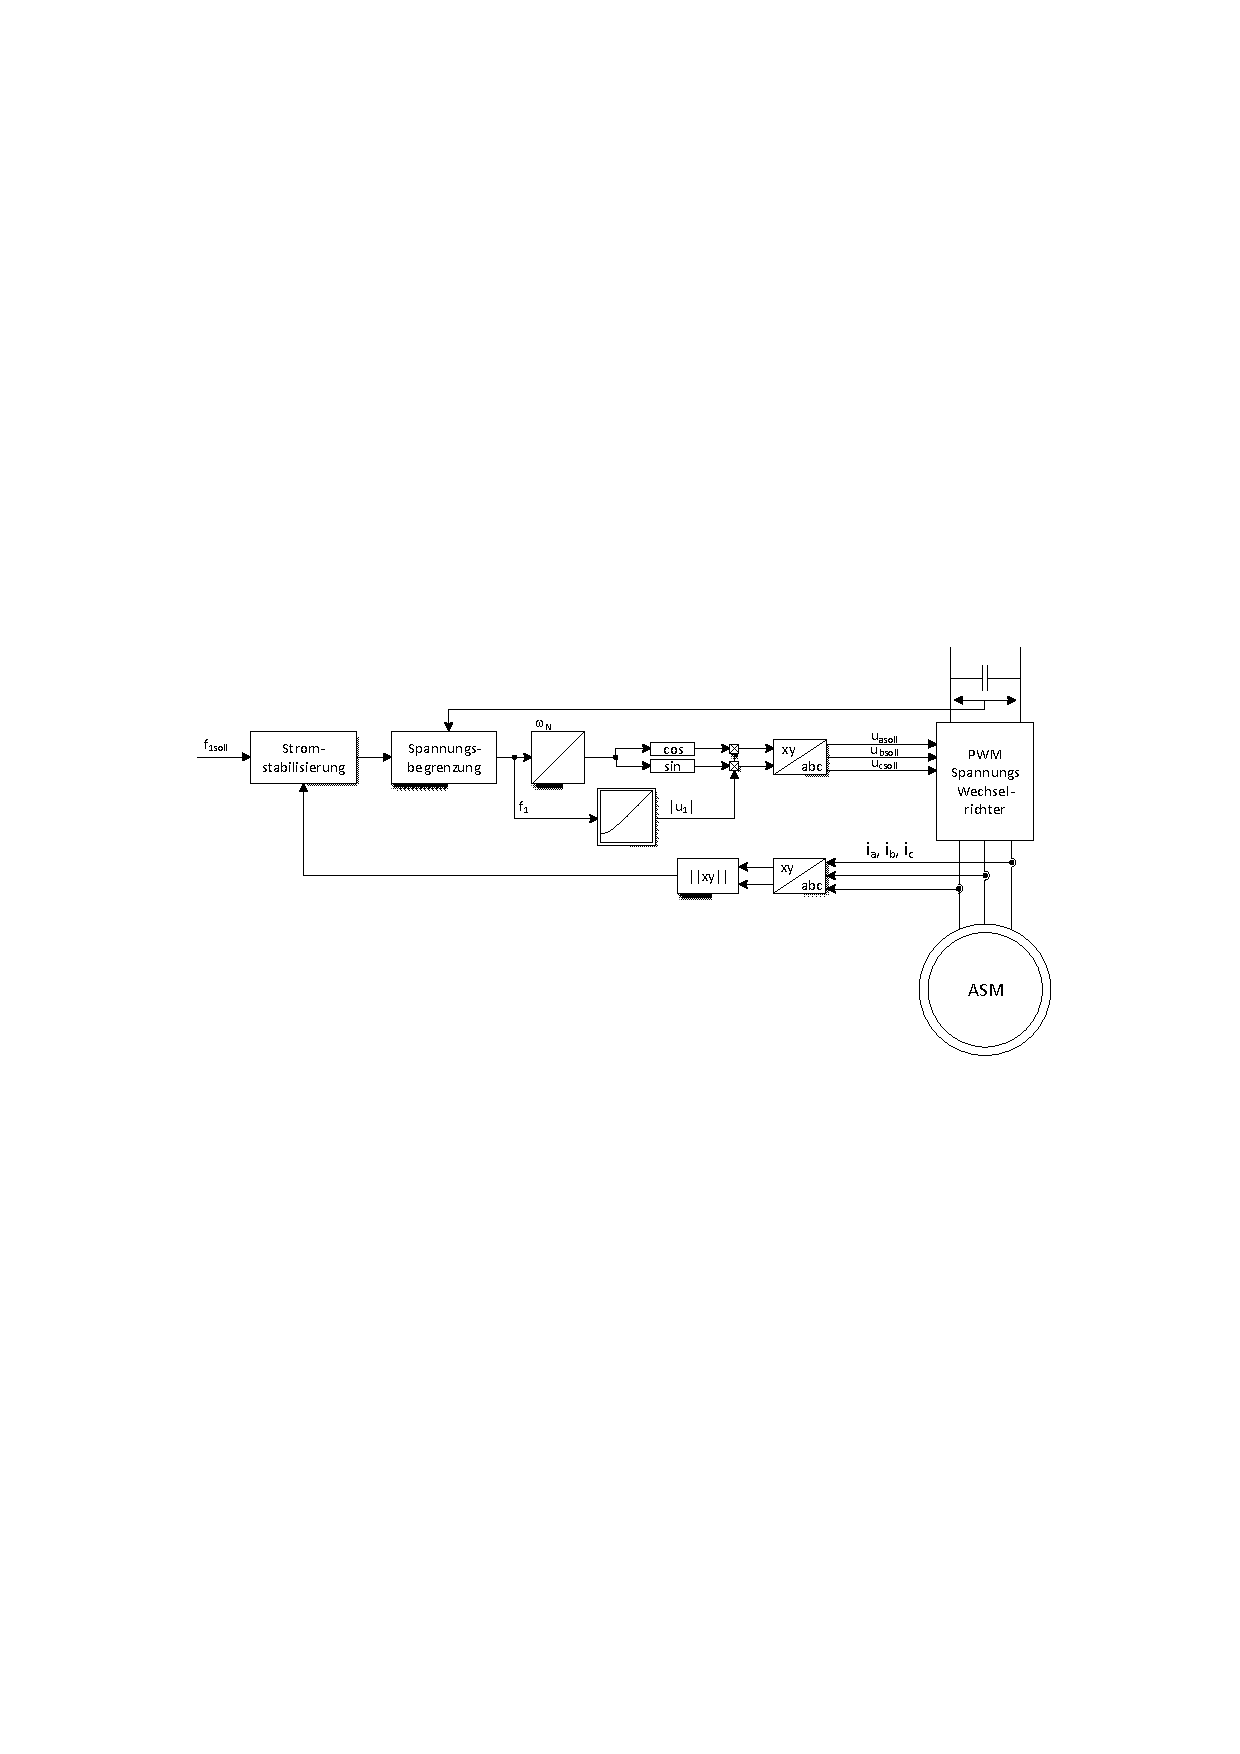
\includegraphics[width=\columnwidth]{Uf.pdf}

Steuerung der Statorfrequenz durch anlegen einer bestimmten Maschinenspannung.

Keine präzise Einstellung der Drehzahl, da Schlupf (abhängig vom Drehmoment). Schlupfkompensation durch Strommessung möglich.

Einfaches Steuerverfahren da keine Schätzung der internen Zustandsgrössen. Aber nur bei geringer Dynamik geeignet.


\end{sectionbox}
\begin{sectionbox}

\subsection{Steuerung mit  Drehzahlgeber}

Variante mit Drehzahlgeber möglich: 

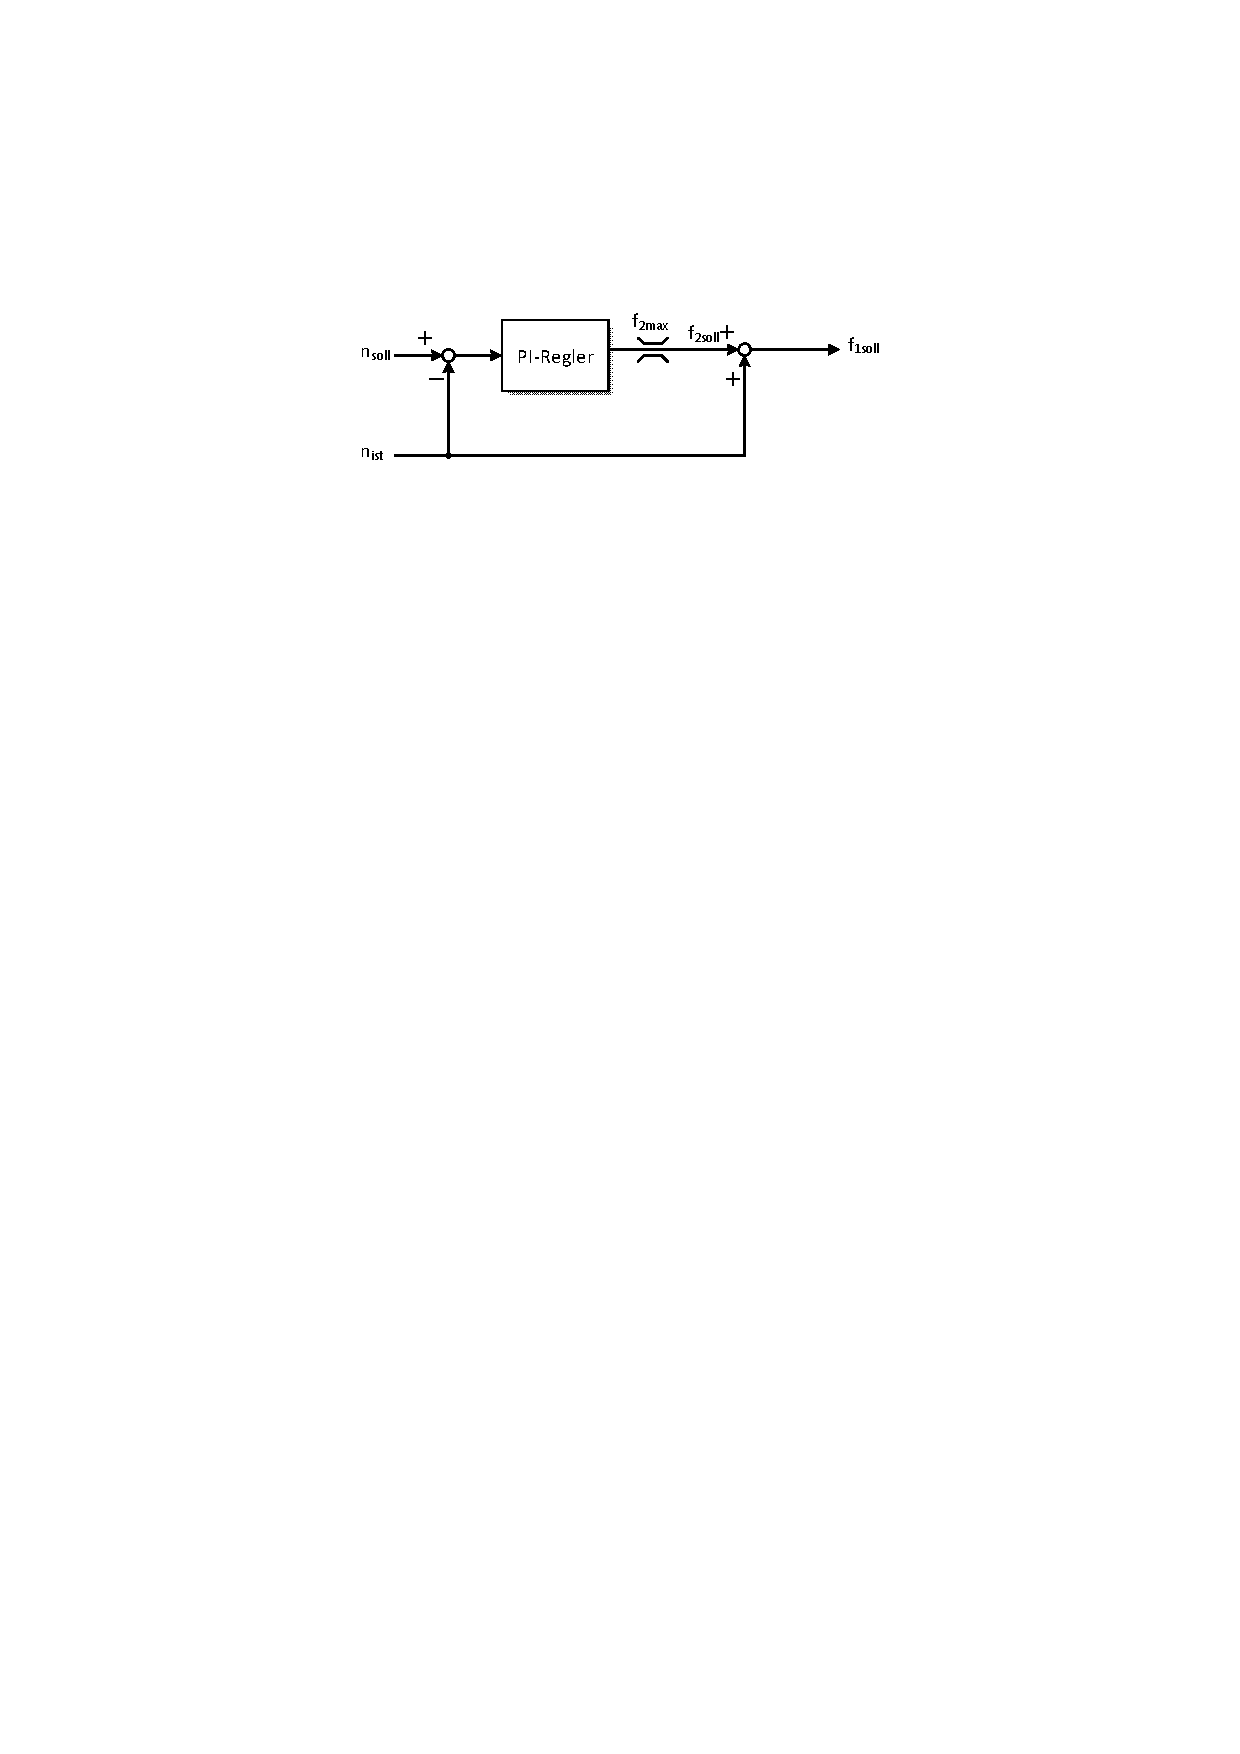
\includegraphics[width=\columnwidth]{Uf_drehzahlgeber.pdf}

Vorteil: Einstellen der Rotorfrequenz ($\ra$ Drehzahl) möglich
\end{sectionbox}

\section{Auslegung von Regelkreisen}
\begin{sectionbox}
\subsection{Regelkreise}
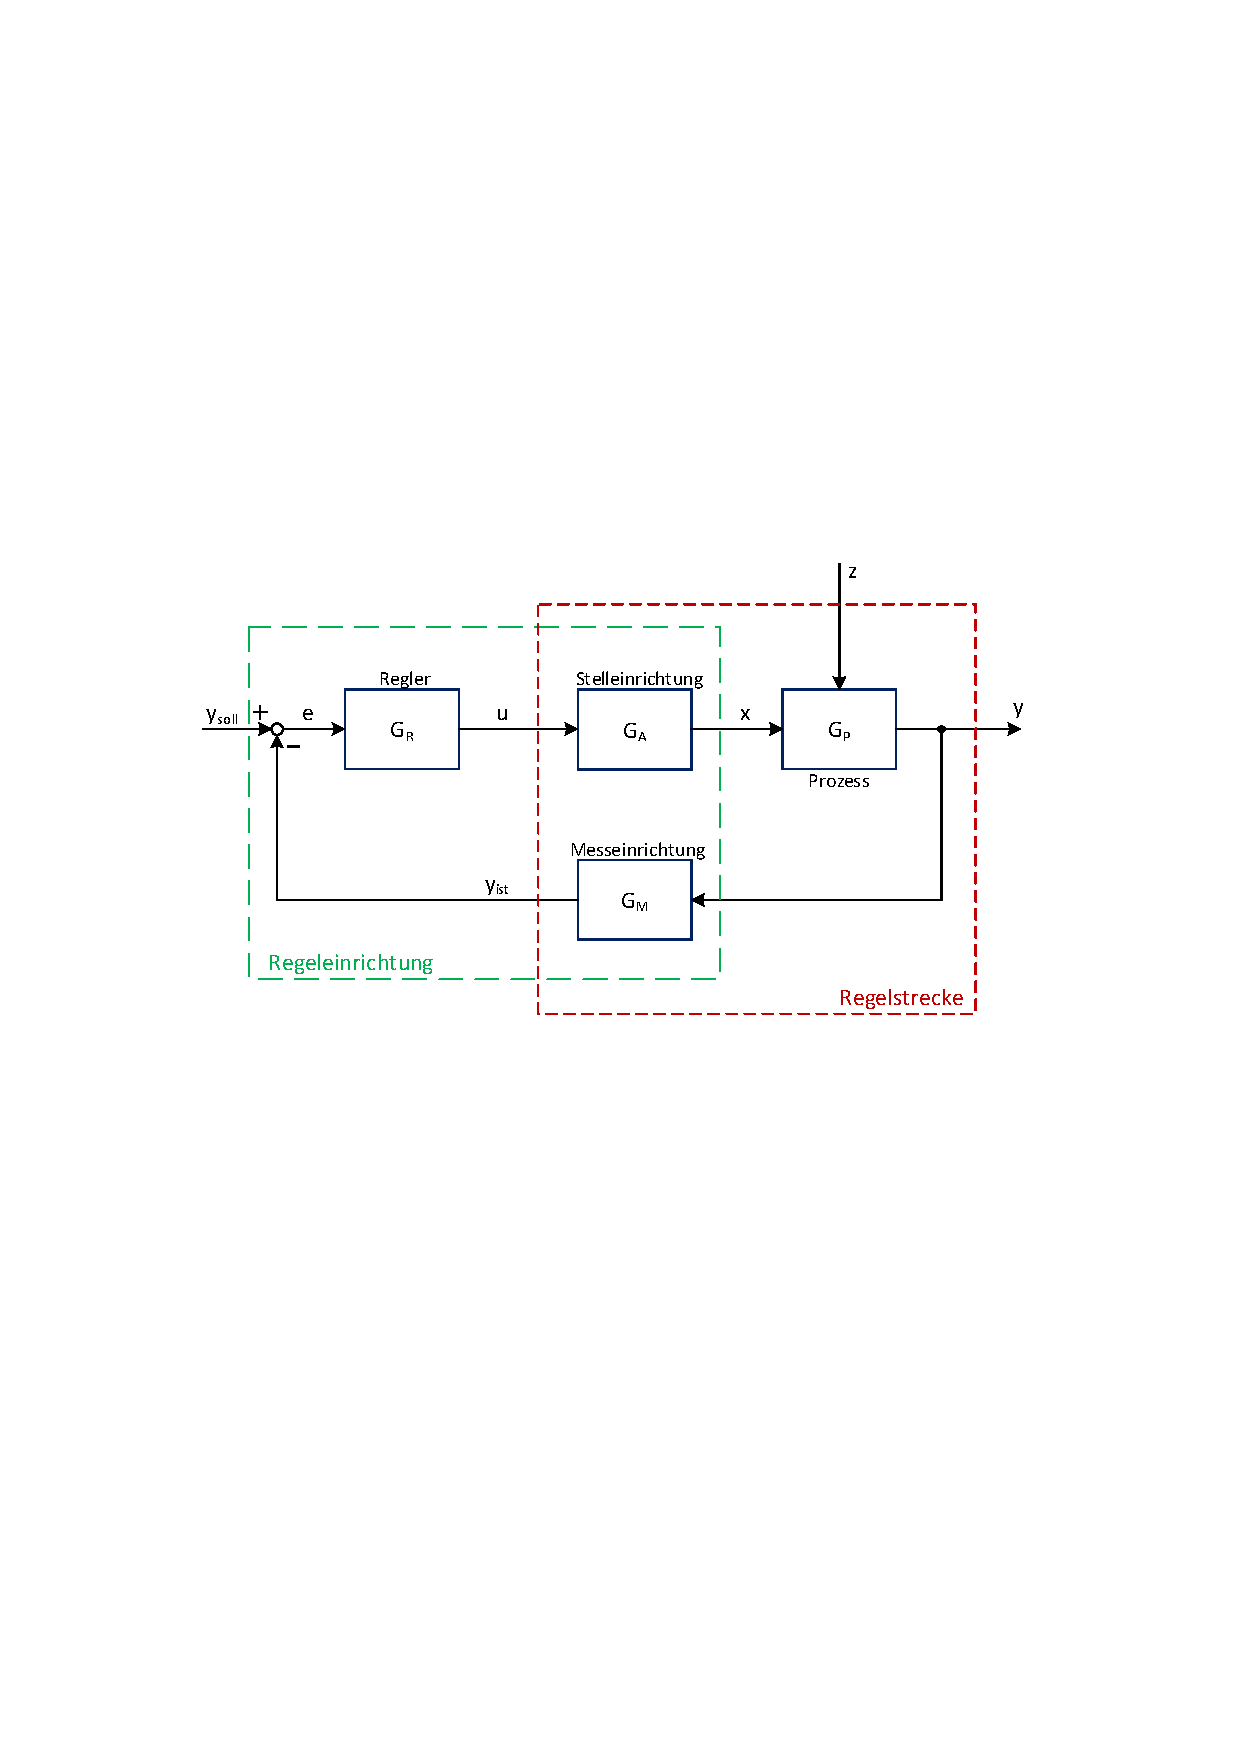
\includegraphics[width=0.8\columnwidth]{Regelkreis.pdf}


Offener Regelkreis: $\vec G_0 (s) = \frac{y(s)}{u(s)} = \vec G_{S1} (s) \cdot \vec G_{S2} (s)$

Offener korrigierter Regelkreis: $\vec G_K (s) = \frac{y(s)}{e(s)} = \vec G_R (s) \cdot \vec G_0 (s)$
\end{sectionbox}
\begin{sectionbox}
\subsection{Stabilität}

\subsubsection{Nyquist Ortskurve}
	
	die Nyquist Ortskurve ist die Frequenzgangortskurve des offenen Regelkreises $G_o (s)$ 
	
	\subsubsection{Nyquist Kriterium}
	
	Betrachtet Nyquist-Ortskurve und Pole $p_{\ir links}, p_{\ir rechts}, p_{\ir auf}$ im Bezug auf die Imaginärachse.
	Das System ist stabil falls die OK nicht durch $-1 + \j 0$ verläuft und die Phasenänderung \\
	
	\begin{emphbox}
	$W_{\ir ist} = \mathop{\Delta}\limits_{\omega = 0}^{\omega \ra \infty} \Phi$
	\end{emphbox}
	
	von $-1 + \j 0$ aus gesehen gleich \\
	
		\begin{emphbox}
		$W_{\ir soll} = \pi p_{\ir rechts} + \frac{\pi}{2} p_{\ir auf}$
		\end{emphbox}
	ist; also $W_{\ir soll} \stackrel{!}{=} W_{\ir ist}$ 
\end{sectionbox}
\begin{sectionbox}
\subsection{Betragsoptimum}
$K_R = \frac{T_{S1}}{2 K_S T_{S \sum}}$

$T_R = T_{S1}$

Zeitkonstante des Reglers kompensiert die grösste Zeitkonstante der Strecke.

\end{sectionbox}
\begin{sectionbox}
\subsection{Symmetrisches Optimum}
$K_R = \frac{T_{S1}}{2 K_S T_{S \sum}}$

$T_R = 4 \cdot T_{S \sum}$

Zeitkonstante des Reglers kompensiert die Summe der kurzen Zeitkonstanten.

\end{sectionbox}
\begin{sectionbox}

\subsection{Stationäre Genauigkeit} 

Im stationären Betrieb soll der Regelfehler sehr klein werden:
$e (t \ra \infty) = 0$

Im Frequenzbereich:
$e (t \ra \infty) = \lim \limits_{s \ra 0} s \cdot e(s) = \frac{1}{1 + \vec G_K (0)}$
\end{sectionbox}

\begin{sectionbox}
\subsection{Frequenzgangfunktion  $G(\j \omega)$}
Beschreibt die Auswirkungen von sinusförmigen Anregungen auf die Systemantwort.

Die Auswirkungen auf Amplitude $A$ und Phasenverschiebung $\varphi$ ergeben die Frequenzgangfunktion $G(\j \omega)$

	\begin{emphbox}
	$G(\j \omega) = A(\omega) e^{\j \varphi (\omega)} = \Re {G(\j \omega)} + \j \Im{G(\j \omega)}$ 
	\end{emphbox}
	\pbox{4cm}{ 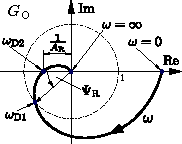
\includegraphics{./img/OK_GO.pdf} } \quad
	\pbox{4cm}{
		\emph{Einschwingzeit:} $T_{\ir Ein} \approx \frac{3}{\omega_{\ir D1}}$\\
		\\
		Stabilitätskriterien mit Totzeit:\\
		geschl. RK ist E/A \textbf{stabil} falls:\\
		Phasenrad $\Phi_{\ir R} > 0$\\
		Amplitudenrand $A_{\ir R} > 1$\\
		\\
		$\Psi_{\ir R} \approx 30^\circ \Leftrightarrow $ gutes Störverhalten\\
		$\Psi_{\ir R} \approx 60^\circ \Leftrightarrow $ gutes Folgeverhalten
	}

	\begin{tabular}{@{}ll@{}}
	\textbf{Kenngrößen:} & Bodediagramm:\\ \mrule
		Amplituden-Durchtrittsfrequenz $\omega_{D1}$: & $A(\omega_{D1}) = 1$\\
		Phasen-Durchtrittsfrequenz $\omega_{D2}$ & $\varphi (\omega_{D2}) = - \pi = -180^\circ$\\
		Phasenrand/Phasenreserve $\Psi_R$: & $\Psi_R = \varphi (\omega_{D1}) + \pi$\\
		Amplitudenrand/-reserve $A_R$ $(= K_{\ir krit})$ & $\frac{1}{A_R} = A (\omega_{D2})$
	\end{tabular}
\end{sectionbox}
\begin{sectionbox}
\subsection{P-Regler}
$\vec G_R (s) = \vec G_P (s) = K_R$

Design: Ändere die Durchtrittsfrequenz $\omega_D$ durch ändern von $K_R$ so, dass der gewünschte Phasenrand entsteht. \\

Für eine Strecke mit Tiefpasscharakteristik und 2 Zeitkonstanten:

$\varphi_{VZ1} = - \arctan (\omega T_{S2})$ \\
$\omega_D = \frac{1}{T_{S2}} \cdot \tan (\frac{\pi}{2} - \varphi_R)$

$\Ra K_R = \frac{\omega_D T_{S1}}{K_S}$
\end{sectionbox}
\begin{sectionbox}
\subsection{PI-Regler}

$\vec G_R (s) = \vec G_{PI} (s) = K_R \cdot \frac{1 + s T_R}{s T_R}$  

Phasendrehung durch Integrator wird für hohe Frequenzen kompensiert.

Knickfrequenz $T_R$ und Verstärkung $K_R$ können unabhänig voneinander eingestellt werden. \\

Für eine Strecke mit Tiefpasscharakteristik und 2 Zeitkonstanten:

Setze die Zeitkonstante $T_R$ auf die grösste Zeitkonstante der Strecke:
$T_R = T_{S1}$. Stelle die Phasenreserve über $K_R$ ein (vgl. P-Regler).

\end{sectionbox}
\begin{sectionbox}

\subsection{PID-Regler}

$\vec G_{PID} (s) = K_R \cdot \frac{1 + s T_{R1}}{s T_{R1}} \cdot \frac{1 + s T_{RD1}}{1 + s T_{RD2}}$ mit $T_{RD1} > T_{RD2}$ 

Phasenanhebende Funktion kann die Phasenreserve erhöhen.

Verhältnis der Knickfrequenzen: $k_{12} = \frac{T_{RD1}}{T_{RD2}}$

Maximaler Phasenwinkel: $\varphi_{\ir max} = \arctan (\sqrt{ k_{12}}) - \arctan (\frac{1}{\sqrt{k_{12}}})$

\end{sectionbox}

\section{Modellierung der Asynchronmaschine}

\begin{sectionbox}
Gleichungen der Asynchronmaschine siehe Kapitel \ref{sec:async}.

Streukoeffizient: $\sigma = 1 - \frac{L_m^2}{L_1 L_2}$
\end{sectionbox}

\begin{sectionbox}
\subsection{Bezugsgrössen}

Spannung: $\hat U_N = \sqrt{\frac{2}{3}} U_{\ir nom, rms} $


Strom: $\hat I_N = \sqrt 2 I_{\ir nom, rms}$

Frequenz: $\omega_N = 2\pi f_{\ir nom}$

Scheinleistung: $S_N = \frac{3}{2} U_N I_N$

Wirkleistung: $P_N = S_N \cdot \cos(\varphi_{\ir nom})$

Fluss: $\Psi_N = \frac{U_N}{I_N}$

Drehmoment: $M_N = \frac{S_N}{\Omega_N} = \frac{3 p }{2} \cdot \Psi_N \cdot I_N$

Impedanz: $Z_N = \frac{U_N}{I_N}$

Kapazität:$ C_N = \frac{1}{\omega_N Z_N}$

Mechanische Drehzahl: $\Omega_N = \frac{\omega_N}{p}$ \\

Per-Unit System:
$x_{\ir p.u.} = \frac{X_{S1}}{X_N}$
\end{sectionbox}


\begin{sectionbox}
\subsection{Statorfestes Koordinatensystem}

$\vec u_1^0 = r_1 \vec i_1^0 + \frac{1}{\omega_N} \cdot \frac{\diff \vec \Psi_1^0}{\diff t}$

$\vec u_2^0 = 0 = r_2 \vec i_2^0 + \frac{1}{\omega_N} \cdot \frac{\diff \vec \Psi_2^0}{\diff t} - \j n \vec \Psi_2^0$

Da $r_2 \vec i_2^0$ klein:

$\frac{\diff \vec \Psi_2^0}{\diff t} = \j n \omega_N \cdot \vec \Psi_2^0 \Ra \vec \Psi_2^0 = \vec{\hat \Psi_2^0} \cdot \e^{\j n \omega_N t}$

$\vec i_2 = \frac{1}{x_m} (\vec \Psi_1 - x_1 \vec i_1)$

$\vec \Psi_2 = \frac{x_2}{x_m} (\vec \Psi_1 - \sigma x_1 \vec i_1)$ mit $\sigma = 1 - \frac{x_m^2}{x_1 x_2}$

\end{sectionbox}
\begin{sectionbox}
\subsection{Rotorflussorientiertes Koordinatensystem}

$\vec u_2^R = 0 = r_2 \vec i_2^R + \frac{1}{\omega_N} \cdot \frac{\diff \Psi_2^R}{\diff t} + \j (f_1^R - n) \vec \Psi_2^R$

$\vec i_2 = \frac{1}{x_2} (\vec \Psi_2 - x_m \vec i_1)$

$\frac{\diff \vec \Psi_2^R}{\diff t} = (- \frac{1}{T_2} - \j f_2^R \omega_N) \cdot \vec \Psi_2^R + \frac{1}{T_2} x_m \vec i_1^R$ 

Rotorzeitkonstante: $T_2 = \frac{L_2}{R_2} = \frac{x_2}{\omega_N r_2}$

Rotorfrequenz (Schlupffrequenz): $f_2^R = f_1^R - n$

Da $d$-Achse in Richtung des Rotorflusszeigers $\vec \Psi_2$ orientiert:

$\vec \Psi_2^R = \Psi_{2d}^R = \Psi_2$

$\Ra \frac{\diff \Psi_2}{\diff t} = - \frac{1}{T_2} \Psi_2 + \frac{1}{T_2} \cdot x_m i_{1d}^R$
\end{sectionbox}


\section{Rotorflussorientierte Regelung} 

\begin{sectionbox}

\subsection{Direkte Rotorflussorientierung} 

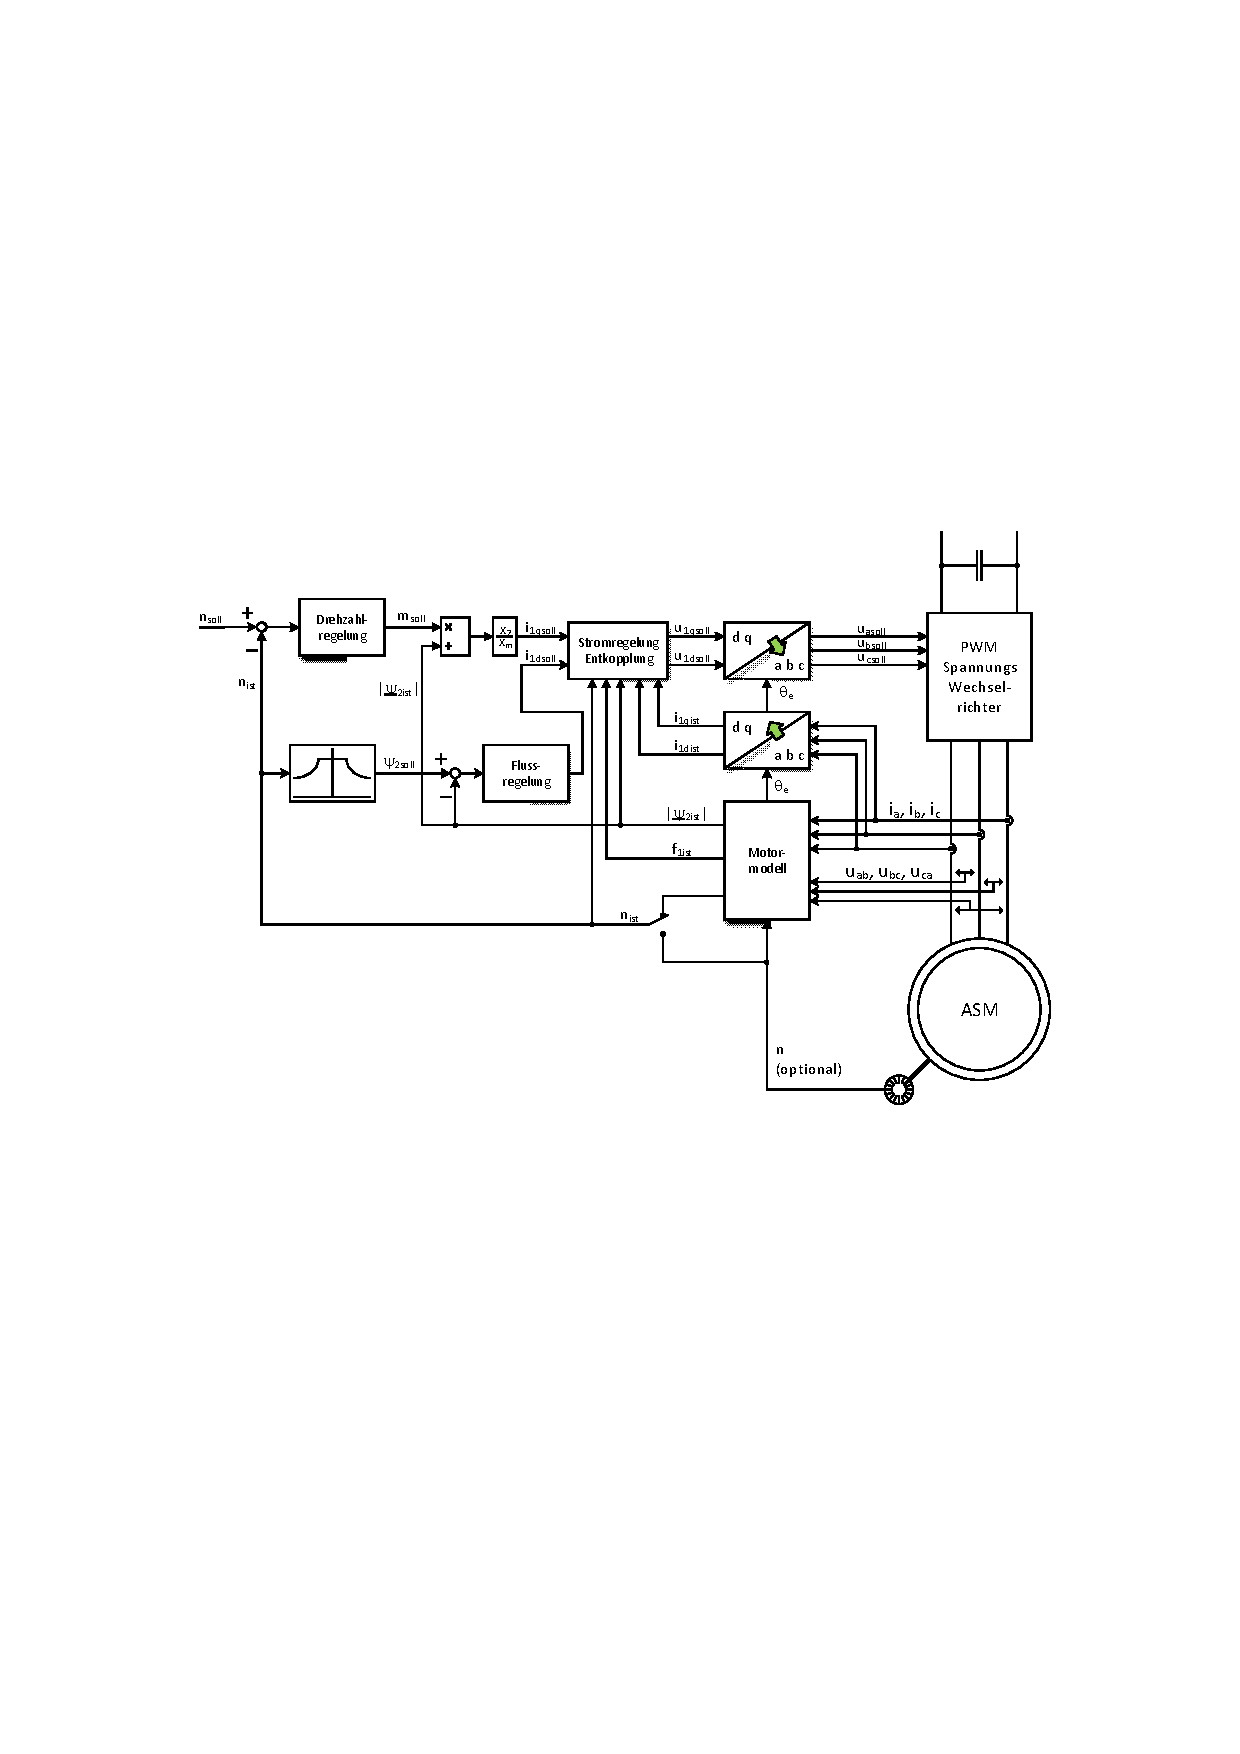
\includegraphics[width=\columnwidth]{direktRFORegelung.pdf}


$i_{1d \ir soll} = \frac{1}{x_{m} \Psi_{2\ir soll}}$
\end{sectionbox}

\begin{sectionbox}

\subsection{Phase-Locked Loop (PLL)} 

Ziel: Finden des Transformationswinkels in das d-q Koordinatensystems
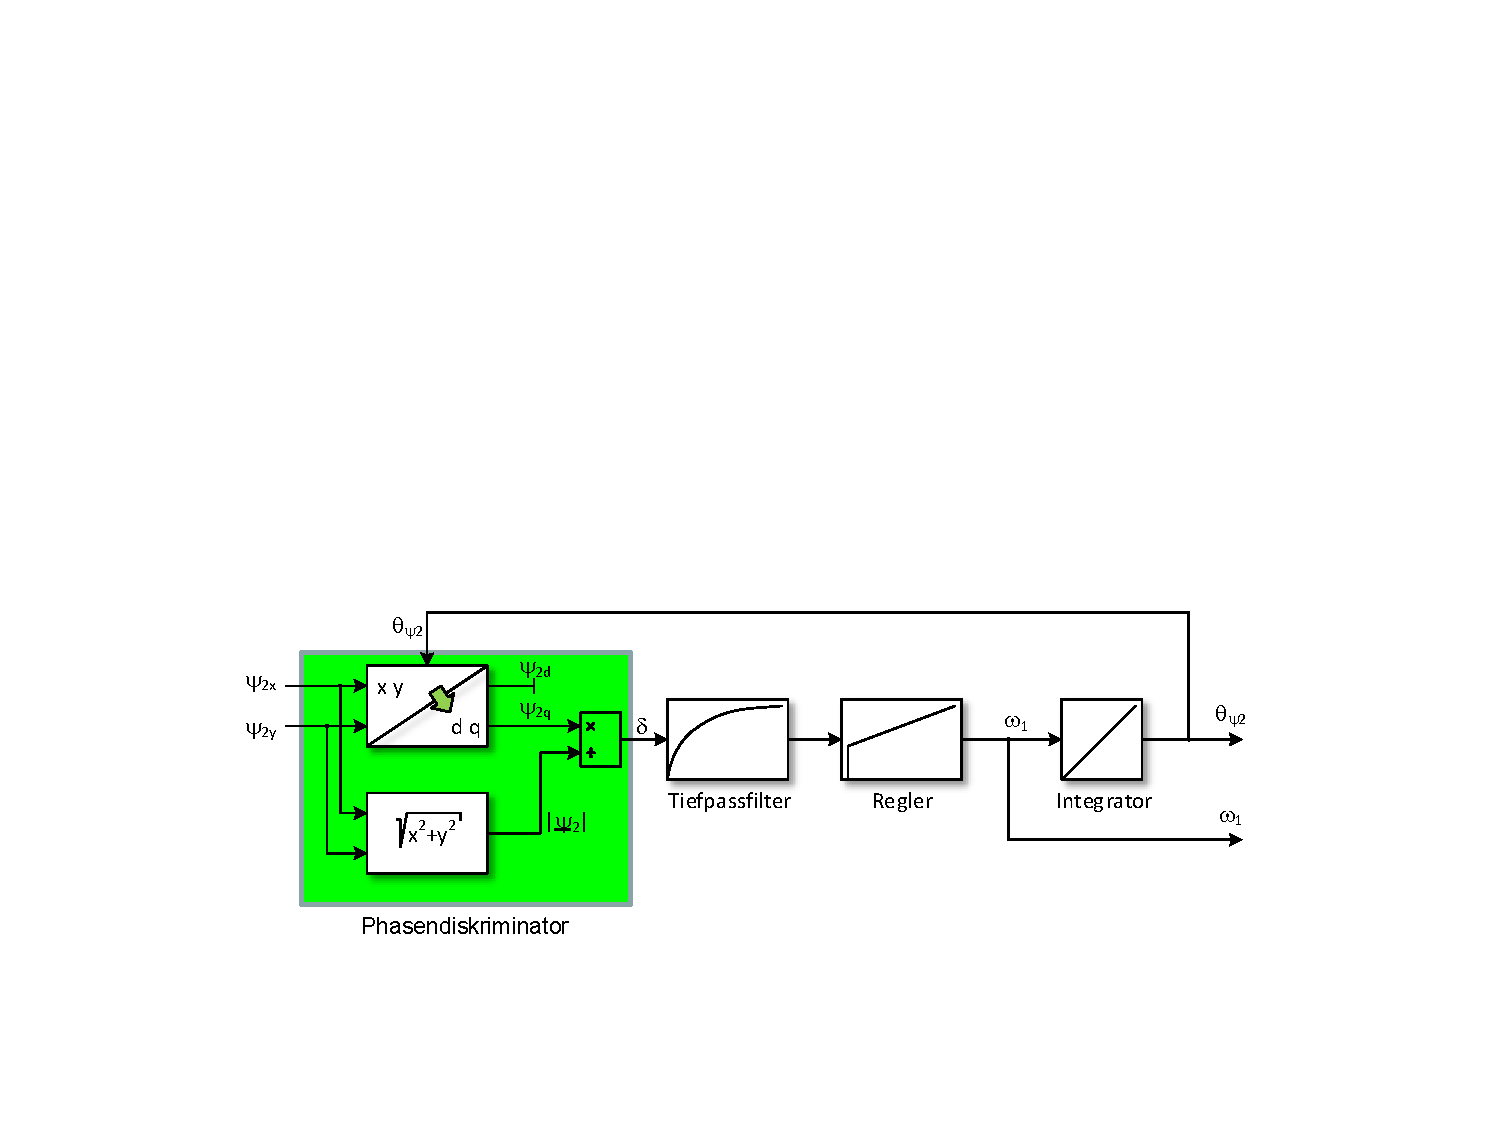
\includegraphics[width=\columnwidth]{PLL.pdf}
\end{sectionbox}
\begin{sectionbox}

\subsection{Indirekte Rotorflussorientierung} 
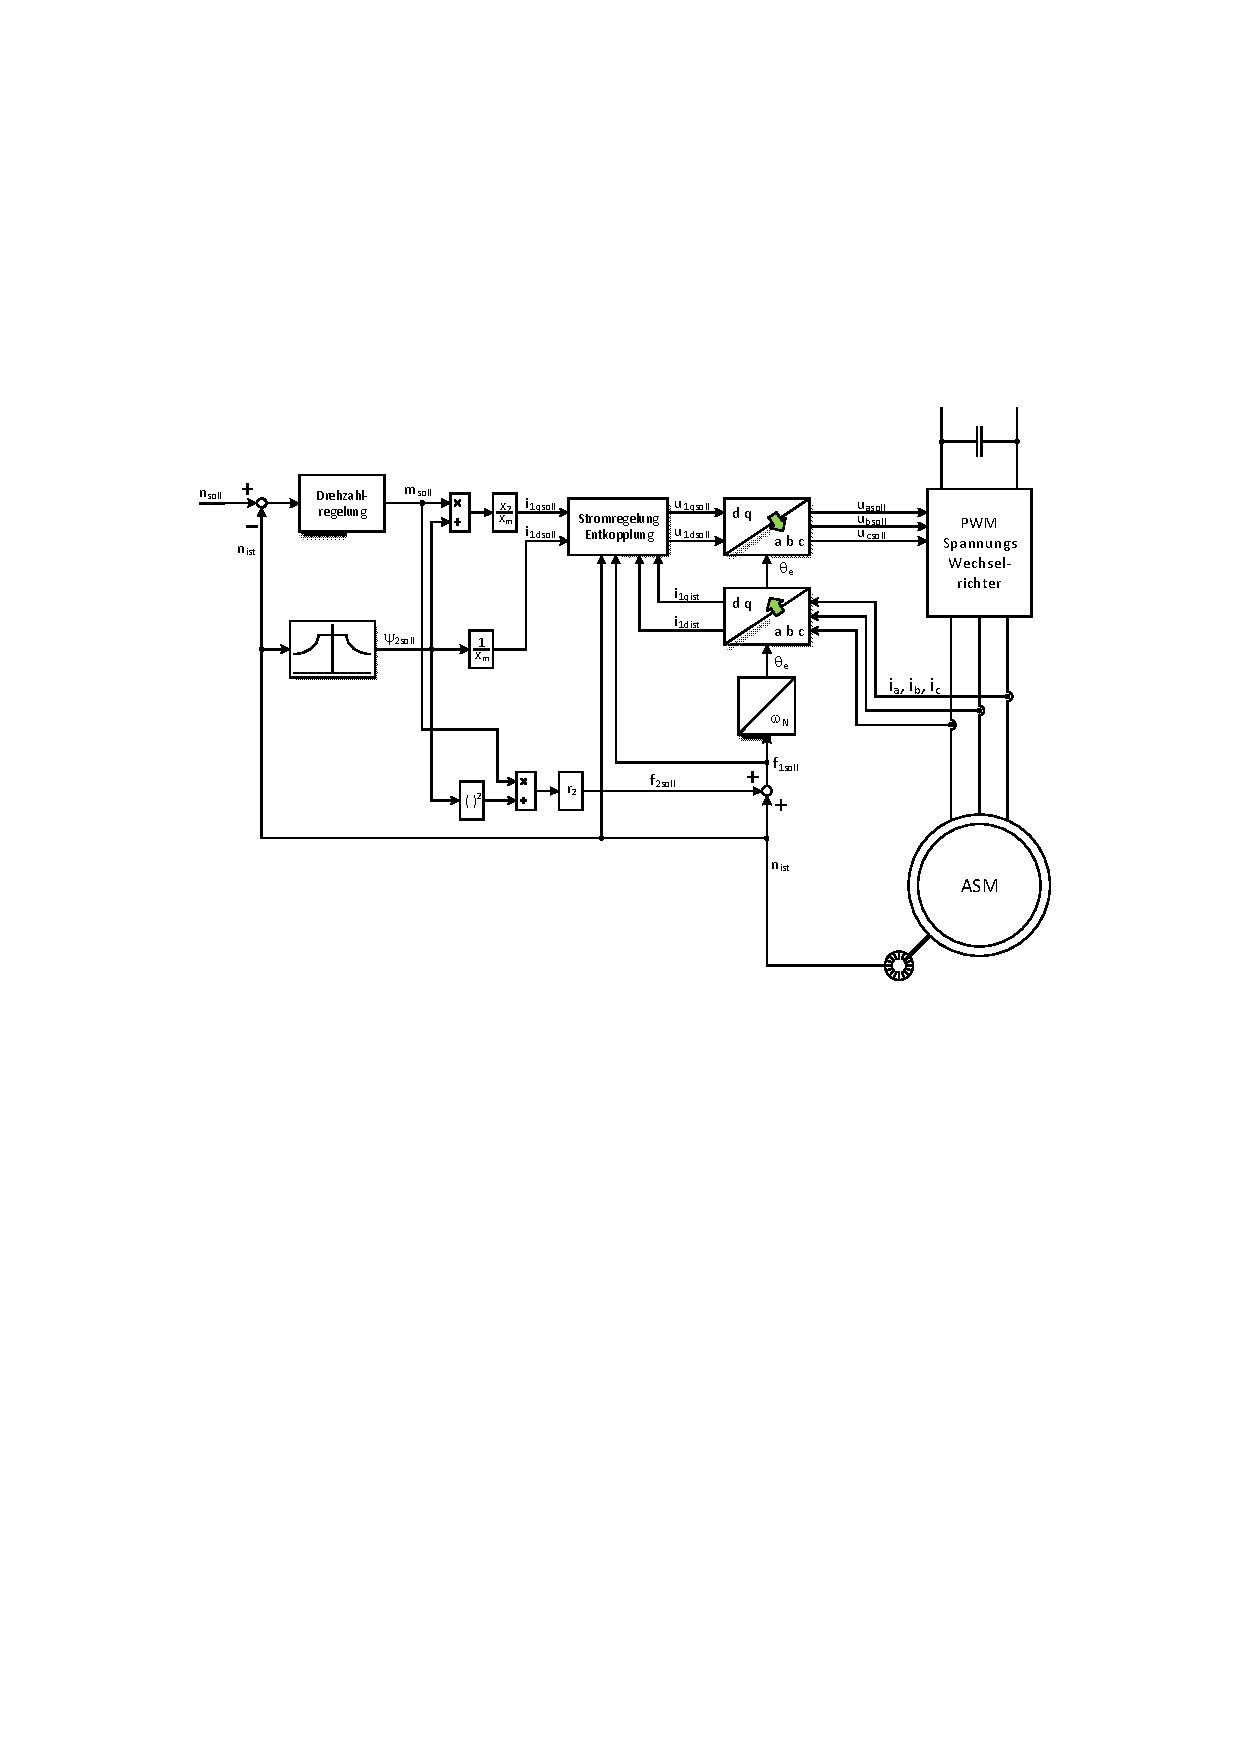
\includegraphics[width=\columnwidth]{indirektRFORegelung.pdf}
\end{sectionbox}
\begin{sectionbox}
\subsection{Stromregelung}
\includegraphics[width=\columnwidth]{iregelung.pdf}

Verzögerungszeit des Modulators: $T_{t, \ir mod} = \frac{1}{4 \cdot f_{\ir carrier}}$ (Unterschwingungsverfahren)

Übertragungsfunktion: $\frac{u_{1d'}^R}{u_{1d \ir soll'}^R} = e^{- s T_{t \ir mod}} \approx \frac{1}{1 + s T_{t \ir mod}}$\\
(da Totzeit $\ll$ Zeitkonstanten des Regelkreises)

\subsubsection*{Strecke} $\frac{i_{1d}^R}{u_{1d'}^R} = \frac{1 / r_e}{1 + s \frac{\sigma x_1}{\omega_N r_e}} = \frac{k_c}{1 + sT_c}$ mit $k_c = \frac{1}{r_e}$, $T_c = \frac{\sigma x_1}{\omega_N r_e}$

\subsubsection*{Messeinrichtung}
$\frac{i_{1 \ir dist}^R}{i_{1d}^R} = \frac{1}{(1 + s T_{fc})} e^{-s T_{tc}} \approx \frac{1}{(1 + s T_{fc}) (1 + s T_{tc})}$ 

\subsubsection*{Regler}

$T_{Rc} = T_c  = \frac{\sigma x_1}{\omega_N r_e}$ (Betragsoptimum)

$K_{Rc} = \frac{T_c}{2 k_c T_{\Sigma c}} = \frac{\sigma x_1}{2 \omega_N T_{\Sigma c}}$ 

\subsubsection*{Entkopplung}

$u_{1d}^R = u_{1d}^{R'} - \sigma x_1 f_1^R i_{1q}^R - \frac{1}{\omega_N T_2} \cdot \frac{x_m}{x_2} \Psi_2$

$u_{1q}^R = u_{1q}^{R '} + \sigma x_1 f_1^R i_{1d}^R + n \cdot \frac{x_m}{x_2} \Psi_2$ 

\subsubsection*{Begrenzung}

$i_{1q \ir max} = \sqrt{i_{1\ir max}^2 - i_{1d \ir ist}^2} $ 
\end{sectionbox}
\begin{sectionbox}
\subsection{Flussregelung}
\includegraphics[width=\columnwidth]{Flussregelung.pdf}

\subsubsection*{Strecke}

$\frac{\Psi_2}{i_{1d}^R} = \frac{x_m}{1 + s T_2}$

\subsubsection*{Stromregelkreis}

$\frac{i_{1 \ir dist}^R}{i_{1d \ir soll}^R} = \frac{1}{1 + s T_{ccl}}$

\subsubsection*{Flussregler}
$T_{\Sigma \Psi} = T_{ccl} + T_{\ir beob}$   

$T_{R \Psi} = 4 T_{\Sigma \Psi}$ (Symmetrisches Optimum)

$K_{R \Psi} = \frac{T_2}{2 x_m T_{\Sigma \Psi}}$
\end{sectionbox}
\begin{sectionbox}
\subsection{Drehzahlregelung}
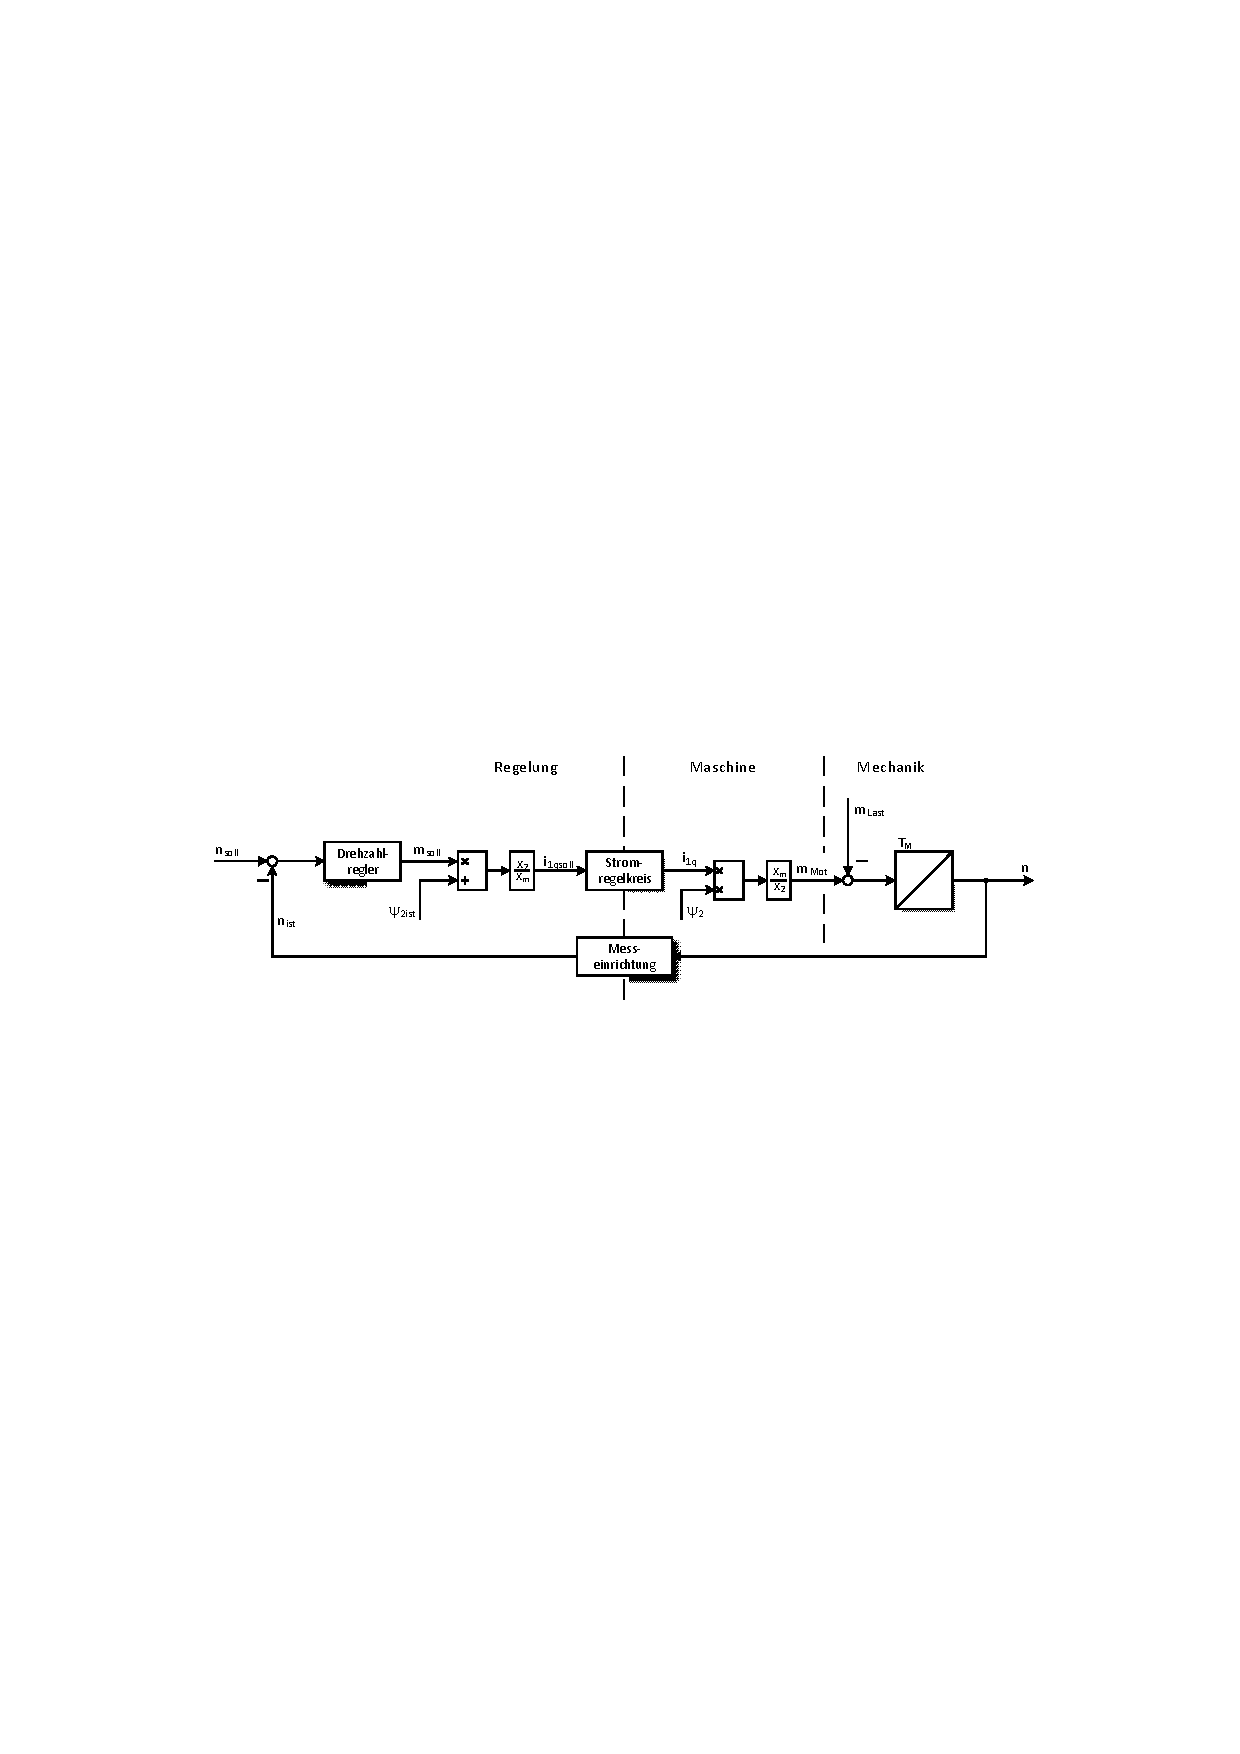
\includegraphics[width=\columnwidth]{Drehzahlregelung.pdf}

\subsubsection*{Strecke}

$T_M = \frac{J_{\ir sum} \cdot \Omega_N}{M_N}$ mit $\Omega_N = \frac{\omega_N}{p}$

$\frac{\diff n}{\diff t} = \frac{1}{T_M} \cdot (m_{\ir Mot} - m_{\ir Last})$

$\frac{m_{\ir ist}}{m_{\ir soll}} = \frac{i_{q \ir ist}}{i_{q \ir soll}} = \frac{1}{1 + s T_{ccl}}$ mit $T_{ccl} = 2 T_{\Sigma c}$ des Stromregelkreises

\subsubsection*{Messeinrichtung} 

Drehzahlgeber oder Drehzahlbeobachter. Tiefpassfilter gegen Störungen, Abtastung u. Rechenzeit ($\ra$ Totzeit)

\subsubsection*{Reglerauslegung}

\emph{Strecke:} \\
$T_{n \Sigma} = T_{ccl} + T_{fn} + T_{ta} + T_{tr}$

$\vec G_o = \frac{1}{s T_M ( 1+ s T_{n \Sigma})}$ 

\paragraph*{P-Regler}

Führungsverhalten: $\frac{n_{\ir ist}}{n_{\ir soll}} = \frac{1}{1 + s \frac{T_M}{K_R} + s^2 \frac{T_M T_{n \Sigma}}{K_R}}$

Störverhalten: $\frac{n_{\ir ist}}{m_{\ir Last}} = \frac{1}{K_R} \cdot \frac{1 + s T_{n \Sigma}}{1 + s \frac{T_M}{K_R} + s^2 \frac{T_M T_{n \Sigma}}{K_R}}$

$\Ra $ Ungeeignet da schlechtes Störverhalten.

$\Ra$ PI-Regler vorteilhaft
\end{sectionbox}
\begin{sectionbox}
\subsection{Positionsregelung}
$\omega_{Dn} = \frac{1}{2 T_{n \Sigma}}$

\end{sectionbox}


\begin{sectionbox}
\subsection{Feldschwächung}    
\end{sectionbox}
\section{Direct Torque Control} 
\begin{sectionbox}
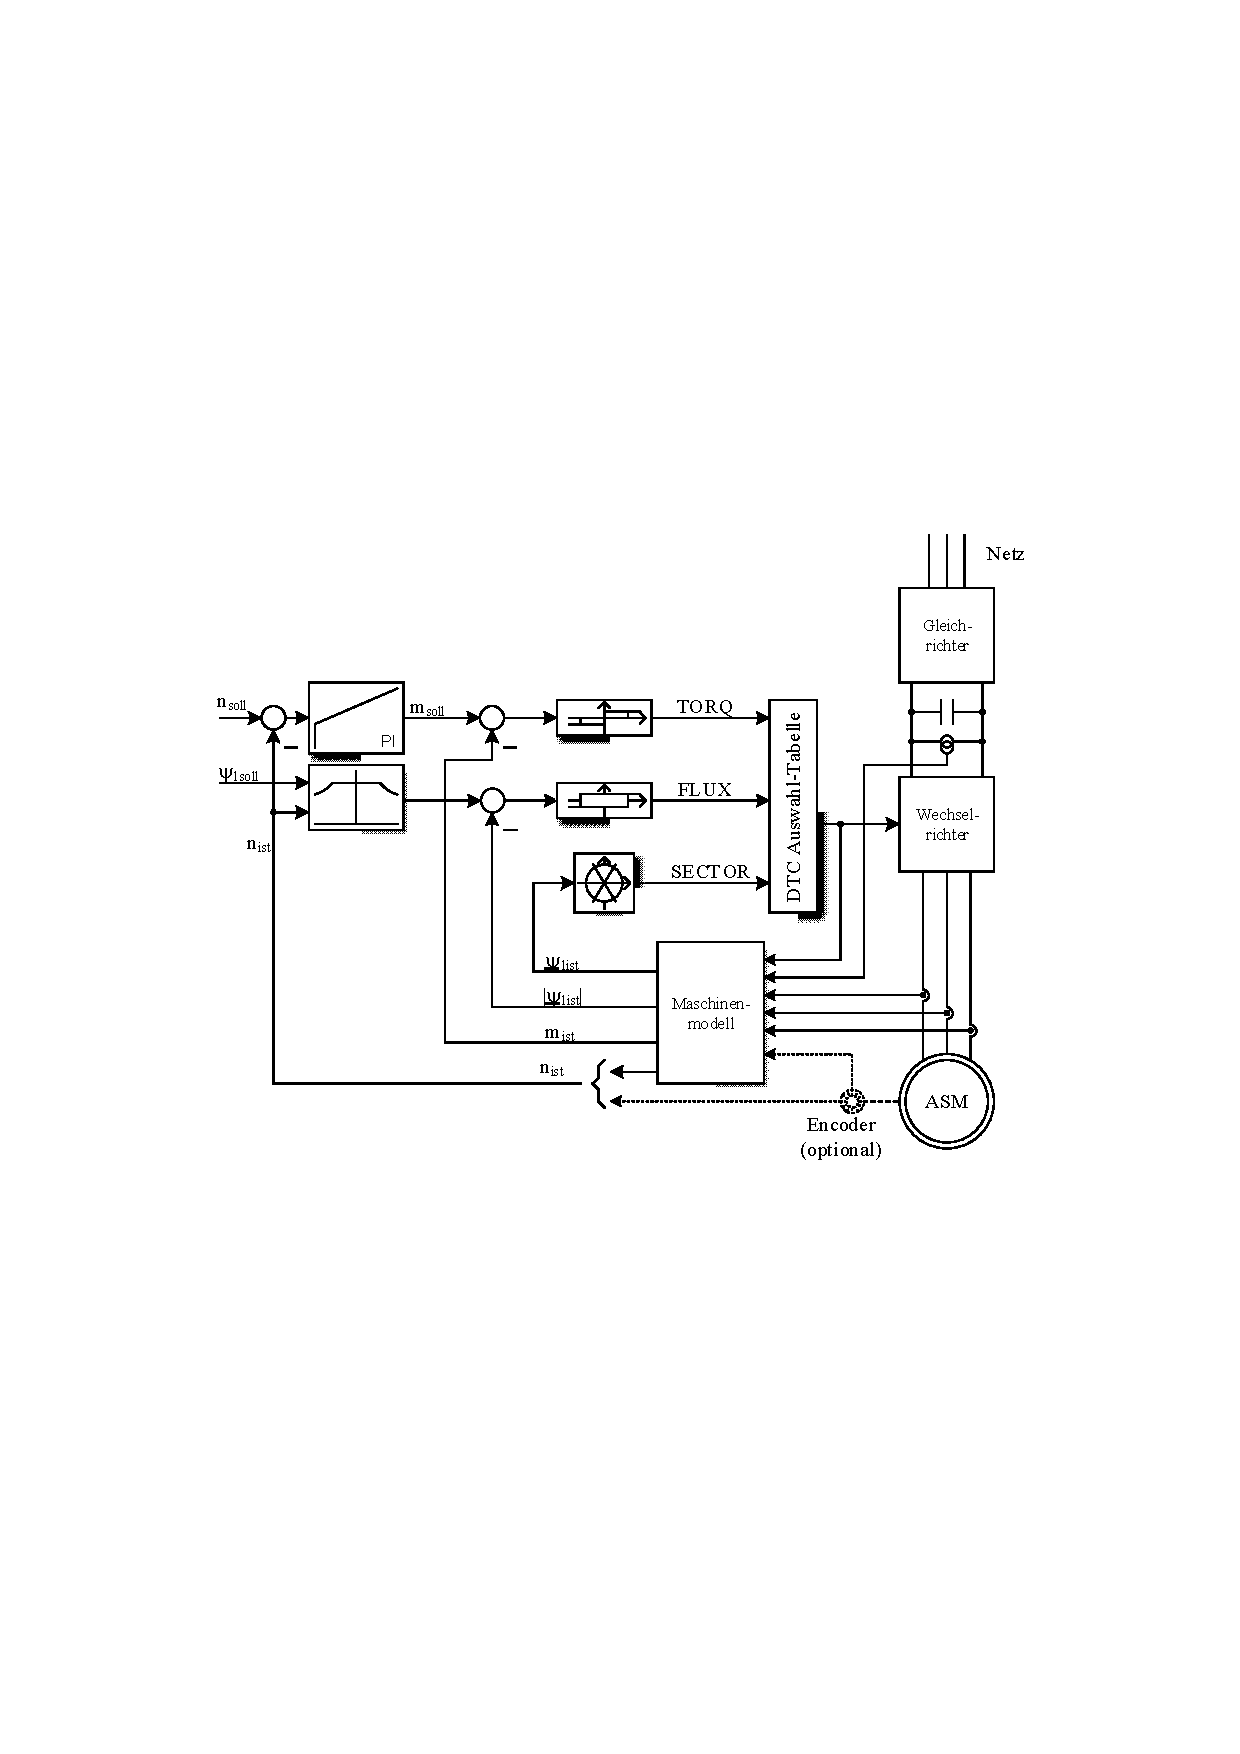
\includegraphics[width=\columnwidth]{DTC.pdf}


Regelung des Drehmoments und des Flusses direkt durch den Schaltzustand (Raumzeiger) des Umrichters.

Bestimme zu jedem Zeitpunkt den Spannungsvektor der Statorfluss und Drehmoment in gewünschter Richtung beeinflusst. \\


Änderung der Flussamplitude: $\frac{\diff \vec \Psi_1}{\diff t} = \omega_N \cdot (\vec u_1 - r_1 \cdot \vec i_1)$

Änderung des Drehmoments: $m_e = \frac{x_m}{\sigma x_1 x_2} \cdot \abs{\vec \Psi_1} \cdot \abs{\vec \Psi_2} \sin \alpha$ \\
$\ra $ Regelung des Drehmoments durch den Winkel des Statorflusszeigers.
\end{sectionbox}

\section{Flussschätzung} 

\begin{sectionbox}
\subsection{Spannungsmodell}

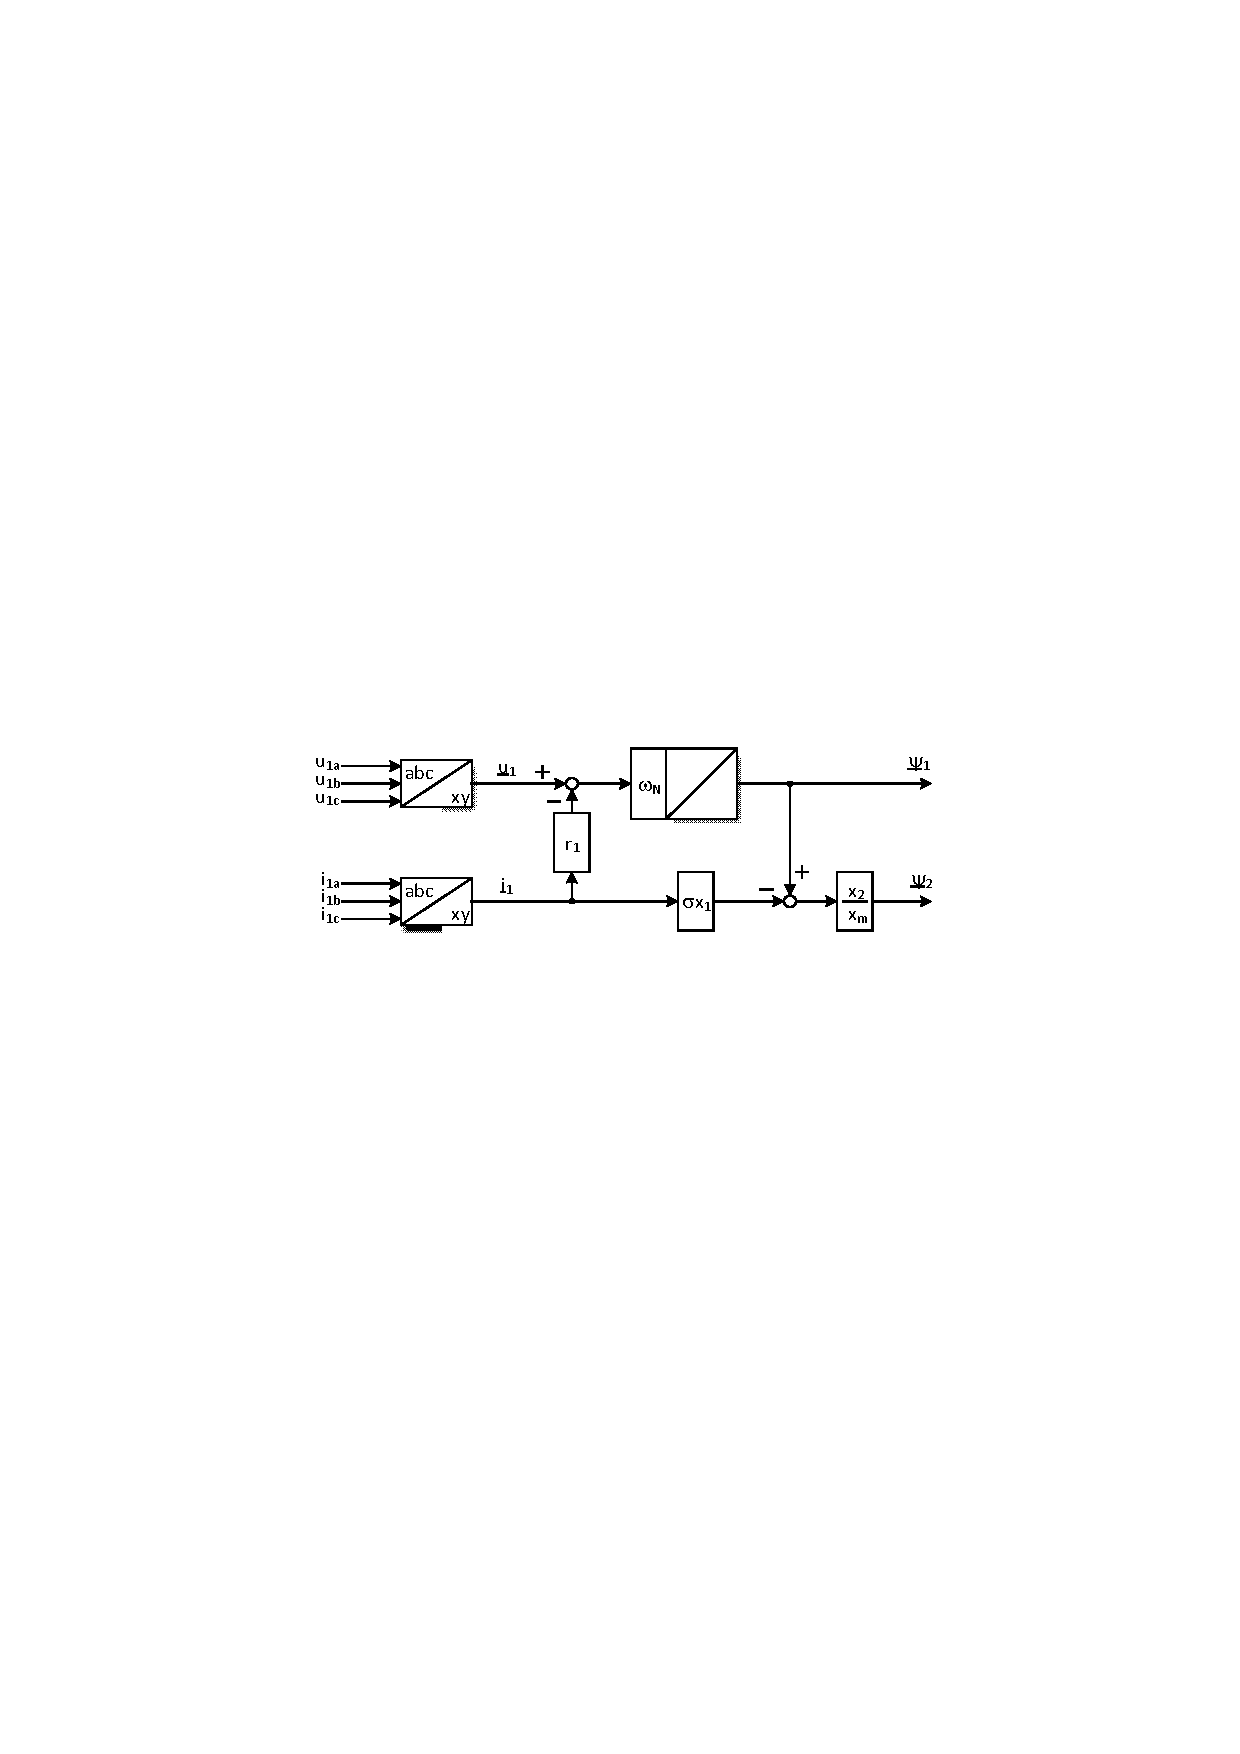
\includegraphics[width=0.8\columnwidth]{Spannungsmodell} 

$\vec u_1^0 = r_1 \vec i_1^0 + \frac{1}{\omega_N} \cdot \frac{\diff \vec \Psi_1^0}{\diff t}$

$\vec \Psi_2 = \frac{x_2}{x_m} (\vec \Psi_1 - \sigma x_1 \vec i_1 )$
\end{sectionbox}

\begin{sectionbox}
\subsection{Strommodell}

Im rotorfesten Koordinatensystem: 
$\frac{\diff \vec \Psi_2^L}{\diff t} = - \frac{1}{T_2} \vec \Psi_2^L + \frac{1}{T_2} x_m \vec i_1^L$
\end{sectionbox}
\end{document}